\chapter{Measurement of the top quark mass at \texorpdfstring{$\sqrts=8$}{sqrt(s)=8}~\TeV}
\label{chap:topmass8TeV}
%
The \tquark\ mass analysis presented in \chap~\ref{chap:topmass7TeV} has been refined and applied to the \gls{ATLAS} dataset, recorded in 2012 with the higher \cme\ of $\sqrts=8$~\TeV. This chapter highlights the differences from the analysis at $\sqrts=7$~\TeV\ and refers back to the definitions and motivations therein wherever possible, to avoid repetition. Extensive documentation about physics objects, calibration, background estimation and \gls{MC} samples is available in \reference~\cite{Acharya:1563201}.

The chapter is organised as follows: 
%
after an introduction to the data and \gls{MC} samples, the different event selections are discussed.
%
The template fits and their application to the data are presented, followed by the identification of the systematic uncertainty sources and an evaluation of their impact on the measurement. 










\section{Data and Monte Carlo samples}
\label{sect:dataMC8TeV}
%
This analysis is based on \pp\ collision data recorded by the \gls{ATLAS} detector in 2012 at a \cme\ of $\sqrts=8$~\TeV. The integrated luminosity amounts to $\intlumi=\atlumo~\invfb$ with an uncertainty of \atlumounc. This was measured using a technique similar to the ones employed for $\sqrts=7$~\TeV\ data in \reference~\cite{Aad:2013ucp}, based on a calibration from beam overlap scans. 

The \gls{MC} simulated event samples have been produced with mostly the same setup as specified in \sect~\ref{sect:dataMC7TeV}, but with the respective change of the beam energy. The integrated luminosity of the central \ttbar\ sample with $\mt=172.5$~\GeV\ is about $\intlumi=360~\invfb$. The effects of \gls{ISRFSR} variations were studied based on \Acermc\ using the CTEQ61 \glspl{PDF} interfaced to \Pythiasix, tuned with the AUET2 instead of the P2011C tune. The \Zj\ background contribution was modelled using \Alpgen\ generated samples interfaced to either \Pythiasix\ or \Herwig, with the same \gls{HFOR} procedure as for the 2011 analysis~\cite{TwikiHFOR}. The \gls{MC} samples were normalised according to the best available cross section calculations, $\sigma_{\ttbar}=253^{+13}_{-15}$~\pb~\cite{CAC-1101,PRL-109-132001,JHEP-1212,JHEP-1301,Czakon:2013goa,CZA-1101} for the \ttbar\ and  $\sigma_\mathrm{t}=87.8^{+3.4}_{-1.9}$~\pb~\cite{Kidonakis:2011wy}, $\sigma_{Wt}=22.4\pm1.5$~\pb~\cite{Kidonakis:2010ux} and $\sigma_\mathrm{s}=5.6\pm0.2$~\pb~\cite{Kidonakis:2010tc} for the single \tquark\ production in the t-, the $Wt$- and the s-channel, respectively.
%
The estimation of the background contributions follows the procedures used for the $\sqrts=7$~\TeV\ analysis. Single \tquark, \Zj, \Wj\ and diboson contributions are estimated from \gls{MC}, as specified in \sect~\ref{sect:dataMC7TeV}. The \fake\ contribution is determined from data using the matrix method, as specified in \sect~\ref{sect:evselreco7TeV}.
%
The uncertainties of the predictions are estimated as the sum in quadrature of the statistical uncertainty, a \atlumounc\ uncertainty on the integrated luminosity, a \xsecunc\ uncertainty on the \ttbar\ cross section, a \stopxsecunc\ uncertainty on the single \tquark\ cross section, a jet multiplicity dependent uncertainty of about 40.0\% on the \Zj\ normalisation and a \qcdunc\ uncertainty on the \fake\ normalisation. Finally, global \JESunc, \bJESunc and \btagunc\ uncertainties are added, corresponding to the envelopes of the results from the eigenvector variations of the \gls{JES}, the \gls{bJES} and the \btag\ scale factors, respectively.
%
These uncertainties apply for all the following tables and figures, unless stated differently.  Distributions normalised to the observed number of data events are shown without the contribution of global uncertainties.









\section{Physics objects}
\label{sect:physobj8TeV}
%
The reconstruction of physics objects in the detector follows the one described in \sect~\ref{sect:physobj7TeV}. 
%
The most important differences with respect to the $\sqrts=7$~\TeV\ objects are specified in the following. 
%
%
\paragraph{Leptons:}\mbox{}
%
As for $\sqrts=7$~\TeV, electron candidates are required to satisfy $\pt>25$~\GeV\ and $\abseta<2.47$~\cite{ATLASCollaboration2014b}.
%
Muon candidates are required to satisfy $\abseta<2.5$ and $\pt > 25$~\GeV\ instead of $20$~\GeV. Also, no pixel detector \blayer\ hits are required and \gls{TRT} hits only in the region $0.1<\abseta<1.9$. 
%
For isolation, instead of the fixed cone requirement, the mini-isolation requirement of $I_\mathrm{mini}<0.05$ is applied, with $I_\mathrm{mini}$ being the ratio of the sum of track \pt\ in a cone of variable radius $\dR = 10~\GeV/\pt^\mu$ around the muon candidate to the transverse momentum of the muon $\pt^\mu$~\cite{Rehermann2011}.
%
%
\paragraph{Jets:}\mbox{}
For the data recorded in 2012, jets are reconstructed using the \gls{LCW} and \gls{GSC} algorithms.
%LCW
The \gls{LCW} procedure is an alternative to the calibration of topological calorimeter clusters to the \gls{EM} scale, which has been used at $\sqrts=7$~\TeV. It locally classifies clusters to be of either hadronic or electromagnetic nature and calibrates them accordingly. In this process, calorimeter non-compensation, limited acceptance and noise contributions are taken into account, following the method described in \reference~\cite{Aad:1409965}.
%GSC
The multivariate \gls{GSC} technique is applied on top of the \gls{LCW}+\gls{JES} calibration. It removes the jet response dependence on a series of variables without changing the average jet energy by a sequential procedure. At each step, the response is reevaluated based on corrected jets from the previous steps to evaluate the next correction~\cite{Aad:1409965}. 
%
This calibration scheme is referred to as the \gls{LCW}+\gls{GSC} calibration. It generally outperforms the \gls{EM}+\gls{JES} calibration scheme in terms of residual \gls{JES} uncertainty, as shown in \reference~\cite{ATLASCollaboration2015b} for $\sqrts=7$~\TeV.
%
% This is shown in \fig{s}~\subref*{sfig:LCWlightdijetJES8TeV} and \subref{sfig:EMlightdijetJES7TeV}, where the fractional \gls{JES} uncertainty as a function of \pt\ for inclusive \ljet{s} in dijet events for the calibrations employed at $\sqrts=8$ and $7$~\TeV\ is displayed. 
% %
% %
% %%%%%%%%%%%%%%%%%%%%%%%%%%%%%%%%%%%%%%%%%%%%%%%%%%%%%%%%%%%%%%%%%%%%%%%%%%%%%%%
% \begin{figure*}[tbp!]
% \centering
% \subfloat[\glsname{LCW}+\glsname{GSC} at $\sqrts=8$~\TeV]{
% 	\includegraphics[width=0.49\textwidth]{./figs/JES_8TeV_LCW_dijet_14a.pdf}
% 	\label{sfig:LCWlightdijetJES8TeV}
% }
% % \subfloat[\gls{EM}+\gls{JES} calibrated jets]{
% % 	\includegraphics[width=0.49\textwidth]{figs/JES_8TeV_EMJES_dijet_14b.pdf}
% % 	\label{sfig:EMlightdijetJES8TeV}
% % }
% \subfloat[\glsname{EM}+\glsname{JES} at $\sqrts=7$~\TeV]{
% 	\includegraphics[width=0.49\textwidth]{figs/JES_7TeV_EMJES_dijet_63a.pdf}
% 	\label{sfig:EMlightdijetJES7TeV}
% }
% \caption[\gls{JES} calibration schemes]{
% %
% The sample-dependent fractional \gls{JES} uncertainty for inclusive \ljet{s} in dijet events as a function of \pt.
% %
% \Fig~\ref{sfig:LCWlightdijetJES8TeV} shows the uncertainty for \glsname{LCW}+\glsname{GSC} calibrated \ljet{s} at $\sqrts=8$~\TeV~\cite{ATLAS-CONF-2015-037}.
% %
% For comparison, the uncertainties for \gls{EM}+\gls{JES} \ljet{s} at $\sqrts=7$~\TeV\ are shown in \fig~\subref{sfig:EMlightdijetJES7TeV}~\cite{ATLASCollaboration2015b}.
% %
% % For comparison, the uncertainties for \gls{EM}+\gls{JES}, the scheme employed for the $\sqrts=7$~\TeV\ analysis, is shown in \fig~\subref{sfig:EMlightJES8TeV}~\cite{ATLAS-CONF-2015-037}.
% %
% \label{fig:JES8TeVschemes}
% }
% \end{figure*}
% %%%%%%%%%%%%%%%%%%%%%%%%%%%%%%%%%%%%%%%%%%%%%%%%%%%%%%%%%%%%%%%%%%%%%%%%%%%%%
% %
%
The pile-up subtraction is performed via the jet area method. This global procedure is based on the observation that pile-up is a uniform and diffuse background, which adds momentum to each jet~\cite{ATLAS-CONF-2013-083}. In this method, the per event average \pt\ density $\rho$ in the $\eta$-$\phi$ plane is determined. This allows the subtraction of the average pile-up momentum from each jet, based on a definition of the jet area using equally distributed artificial particles with negligible \pt\ in the jet clustering, referred to as ghost particles. These ghosts do not influence the clustering of the physical particles, and the number of clustered ghosts over the ghost density represents a measure for the jet area. 
%
Jets originating from local pile-up fluctuations, which are not suppressed below the reconstruction energy threshold by the global pile-up subtraction method, are identified via their \gls{JVF}.
%
The \gls{JVF} requirement of $|\mathrm{\gls{JVF}}|>0.5$ is solely applied to jets with $\pt<50$~\GeV\ and $\abseta<2.4$. Jets outside this phase space are always accepted.
%
Finally, a residual correction for negative energy contributions from \gls{LAr} out-of-time pile-up in high \abseta\ regimes is applied~\cite{ATLAS-CONF-2013-083}.
%
As for $\sqrts=7$~\TeV, jets are required to satisfy $\pt>25$~\GeV\ and $\abseta<2.5$.
%
The \btag\ working point is chosen corresponding to a \btag\ efficiency of 70\% in simulated \ttbar\ events and a \ljet\ (\cjet) rejection factor of 137 (5).
% as $w=0.7892$, 
%https://twiki.cern.ch/twiki/bin/viewauth/AtlasProtected/BTaggingBenchmarks
%










\section{Event reconstruction}
%
The event reconstruction is identical to the one detailed in \sect~\ref{sect:evselreco7TeV}. 
%
The two jets carrying the highest MV1 weight are taken as the two \bjet{s} for the construction of the \mlbr\ estimator. 






Additional studies of discriminative variables confirm the nearly optimal performance of the minimum \mlb\ criterion for the jet to lepton assignment.
%
The performance of the matching algorithms is estimated using \gls{MC} \genlevel\ information to match \recolevel\ objects to the closest \genlevel\ objects.
%
The \genlevel\ matching is performed with a \dR\ requirement of a maximum spatial distance of $\dR^\mathrm{max}_{\ell}=0.1$ for leptons and $\dR^\mathrm{max}_\mathrm{jet}=0.3$ for jets. 
%
Due to acceptance losses and reconstruction inefficiency, not all \recolevel\ objects can successfully be matched to their \genlevel\ counterparts and the corresponding event is denoted as unmatched.
%
The performance is assessed in terms of matching efficiency $\epsilon$ and \selPurity\ $\pi$. The matching efficiency is defined as the fraction of correctly matched over all matched events $\epsilon=\N{c}/(\N{c}+\N{w})$, whereas \selPurity\ denotes the fraction of correctly matched over all events $\pi=\N{c}/(\N{c}+\N{w}+\N{u})$, independently of whether they could be matched or not. The variables $\N{c}$, $\N{w}$, and $\N{u}$ denote the numbers of correctly, wrongly and unmatched events, respectively.
%
%%%%%%%%%%%%%%%%%%%%%%%%%%%%%%%%%%%%%%%%%%%%%%%%%%%%%%%%%%%%%%%%%%%%%%%%%%%%%%%%
\begin{table}[tbp!]
% \footnotesize
\begin{center}
\begin{tabular}{|l|c|c|l|}
\hline
Discriminator                   & $\epsilon$ [\%]  & $\pi$ [\%]   & Assignment strategy    \\ \hline
\mttwo                          & $81.2 \pm 0.2$   & $53.5 \pm 0.1$ & Minimum \mttwo   \\
\mlb                            & $78.4 \pm 0.2$   & $51.6 \pm 0.1$ & Minimum \mlb   \\
$\sum\dR_{j\ell}$               & $73.2 \pm 0.2$   & $48.2 \pm 0.1$ & Minimum sum of $\dR_{j\ell}$    \\
$\prod\dR_{j\ell}$              & $71.9 \pm 0.2$   & $47.3 \pm 0.1$ & Minimum product of $\dR_{j\ell}$    \\
$\pt^\mathrm{max}$              & $71.7 \pm 0.2$   & $47.2 \pm 0.1$ & Maximum jet--lepton system \pt   \\
Random                          & $50.1 \pm 0.1$   & $33.0 \pm 0.1$ & Random choice  \\
\hline
\end{tabular}
\end{center}
\caption[Performance of the matching criteria]{
%
A selection of matching criteria and their performance in terms of matching efficiency $\epsilon$ and \selPurity\ $\pi$ for events with at least one \btagged\ jet. The \mlb\ criterion is used in the analyses.
%
\label{tab:matchcriteria}
}
\end{table}
%%%%%%%%%%%%%%%%%%%%%%%%%%%%%%%%%%%%%%%%%%%%%%%%%%%%%%%%%%%%%%%%%%%%%%%%%%%%%%%%



A set of discriminative variables has been investigated, such as spatial distances between jets and leptons $\dR_{j\ell}$ and their sum and product. Furthermore, $\pt^\mathrm{max}$ and \pt\ balance approaches have been considered, maximising the resulting lepton--\bjet\ system \pt\ or favouring similar \pt\ among top and anti-\tquark\ decay products. 
%
The five best performing variables are given in \tab~\ref{tab:matchcriteria}.
%
A criterion using the transverse mass variable \mttwo~\cite{Barr:2003rg,Lester:1999tx} following the algorithm internal assignment is found to yield slightly higher matching efficiencies than \mlb\ but is not used for simplicity and consistency with the $\sqrts=7$~\TeV\ analysis.













\section{The standard event selection}
\label{sect:evsel8TeV}
%
Since the relevant kinematic event properties remain approximately constant with the change in \cme, the $\sqrts=7$~\TeV\ event selection can also be applied as standard to the $\sqrts=8$~\TeV\ dataset.
%
Therefore, the standard event selection follows the one detailed in \sect~\ref{sect:evselreco7TeV}, but requires events to have at least one \btagged\ jet. The small fraction of events with more than two \btagged\ jets have been included.
%, because they yield an even higher efficiency to select the correct jet--lepton pairs than events with one or two \btagged\ jets.
%
To perform the template parametrisation described in \sect~\ref{sec:templates8TeV}, an additional selection criterion is applied, restricting the measured \mlbr\ to the range  $30~\GeV < \mlbr < 170~\GeV$.  All subsequent tables and figures take this additional criterion into account.
%
The observed numbers of events in the data after the event selection, together with the expected numbers of signal and background events corresponding to the integrated data luminosity, are given in \tab~\ref{tab:stdselDL8TeV}. 
%
Assuming a \tquark\ mass of $\mt=172.5$~\GeV, the predicted number of events is consistent with the one observed in the data within uncertainties. The event yields for the samples with exactly one and exactly two \btagged\ jets are also given. 
%
The matching performance of the \mlb\ reconstruction algorithm in the standard event selection is reported in the bottom rows.
%
In the following, the samples with different \btagged\ jet multiplicity are treated together.
%
%%%%%%%%%%%%%%%%%%%%%%%%%%%%%%%%%%%%%%%%%%%%%%%%%%%%%%%%%%%%%%%%%%%%%%%%%%%%%%%
\begin{table}[tb!]
\begin{center}
\small
\begin{tabular}{|l|rr|rr|rr|}
\hline
Selection &\multicolumn{6}{c|}{Standard event selection} \\  
\hline
\btagged\ jet multiplicity
& \multicolumn{2}{c|}{$=1$ \btagged\ jet} 
& \multicolumn{2}{c|}{$=2$ \btagged\ jets} 
& \multicolumn{2}{c|}{$\ge 1$ \btagged\ jets}\\  
\hline
\ttbar\ signal            & 18800 $\pm$ & 1600 & 14300 $\pm$ & 1200 & 33500 $\pm$ & 2800 \\
Single  \tquark\ (signal) &  1093 $\pm$ &   66 &   377 $\pm$ &   23 &  1477 $\pm$ &   89 \\
\fake{s}                  &   170 $\pm$ &  170 &    61 $\pm$ &   61 &   230 $\pm$ &  230 \\
\Zj\                      &   148 $\pm$ &   56 &  16.6 $\pm$ &  6.8 &   165 $\pm$ &   63 \\
$WW/WZ/ZZ$                &    43 $\pm$ &   15 &  1.36 $\pm$ & 0.63 &    44 $\pm$ &   16 \\
Signal+background         & 20300 $\pm$ & 1600 & 14700 $\pm$ & 1200 & 35400 $\pm$ & 2800 \\ \hline
Data                      & \multicolumn{2}{c|}{19985} 
                          & \multicolumn{2}{c|}{14732} 
                          & \multicolumn{2}{c|}{35099} \\ \hline
Exp. bkg. frac.           & 0.02 $\pm$ & 0.01 & 0.01 $\pm$ & 0.00 & 0.01  $\pm$ & 0.01 \\
Data/MC                   & 0.98 $\pm$ & 0.08 & 1.00 $\pm$ & 0.08 & 0.99  $\pm$ & 0.08 \\
\hline
Matching efficiency $\epsilon$ [\%]    & \effoneb $\pm$ & \effonebunc
													  & \efftwob   $\pm$ & \efftwobunc
													  & \eff   $\pm$ & \effunc \\
\SelPurity\ $\pi$ [\%]          & \fracmatchoneb $\pm$ & \fracmatchonebunc
													  & \fracmatchtwob $\pm$ & \fracmatchtwobunc
													  & \fracmatch $\pm$ & \fracmatchunc \\
Unmatched events [\%]       & \fracunmatchoneb $\pm$ & \fracunmatchonebunc
													  & \fracunmatchtwob $\pm$ & \fracunmatchtwobunc
													  & \fracunmatch $\pm$ & \fracunmatchunc \\
Wrongly matched events [\%] & \fracwrongoneb $\pm$ & \fracwrongonebunc
													  & \fracwrongtwob $\pm$ & \fracwrongtwobunc
													  & \fracwrong $\pm$ & \fracwrongunc \\
\hline
\end{tabular}
\end{center}
\caption[Event yields for $\sqrts=8$~\TeV\ data: standard event selection]{
%
The observed numbers of events in $\intlumi=\atlumo$~\invfb\ of $\sqrt{s} = 8$~\TeV\ data after the standard event selection for different \btagged\ jet multiplicities.
%
Two significant digits are used for the uncertainties of the predictions.
% 
Values smaller than $0.005$ are listed as $0.00$.
%
In addition, the expected numbers of signal and background events corresponding to the integrated luminosity of the data and the matching performance are given with statistical uncertainties only. 
%

%
\label{tab:stdselDL8TeV}
}
\end{table}
%%%%%%%%%%%%%%%%%%%%%%%%%%%%%%%%%%%%%%%%%%%%%%%%%%%%%%%%%%%%%%%%%%%%%%%%%%%%%%%
%



% Distributions of several kinematic variables for the data and the \gls{MC} prediction with $\mt=172.5$~\GeV\ corresponding to the standard event selection are shown in \sect~\ref{sect:distr}, together with the distributions of the optimised event selections.













\section{The optimised event selections}
\label{sect:opti}
Based on the standard event selection described in \sect~\ref{sect:evsel8TeV} without the additional range restriction of the \mlb\ variable, optimisation studies have been performed to improve on the precision of the measurement. 
%
The applied techniques comprise a \oned\ phase space restriction and an \gls{MVA} based selection using a \gls{BDT}. 
%
The former is referred to as \cutbased, the latter as \mvabased\ event selection.
%
%%%%%%%%%%%%%%%%%%%%%%%%%%%%%%%%%%%%%%%%%%%%%%%%%%%%%%%%%%%%%%%%%%%%%%%%%%%%%%%%%%%%%%
\begin{figure*}[tb!]
\centering
\subfloat[\Cutbased]{
  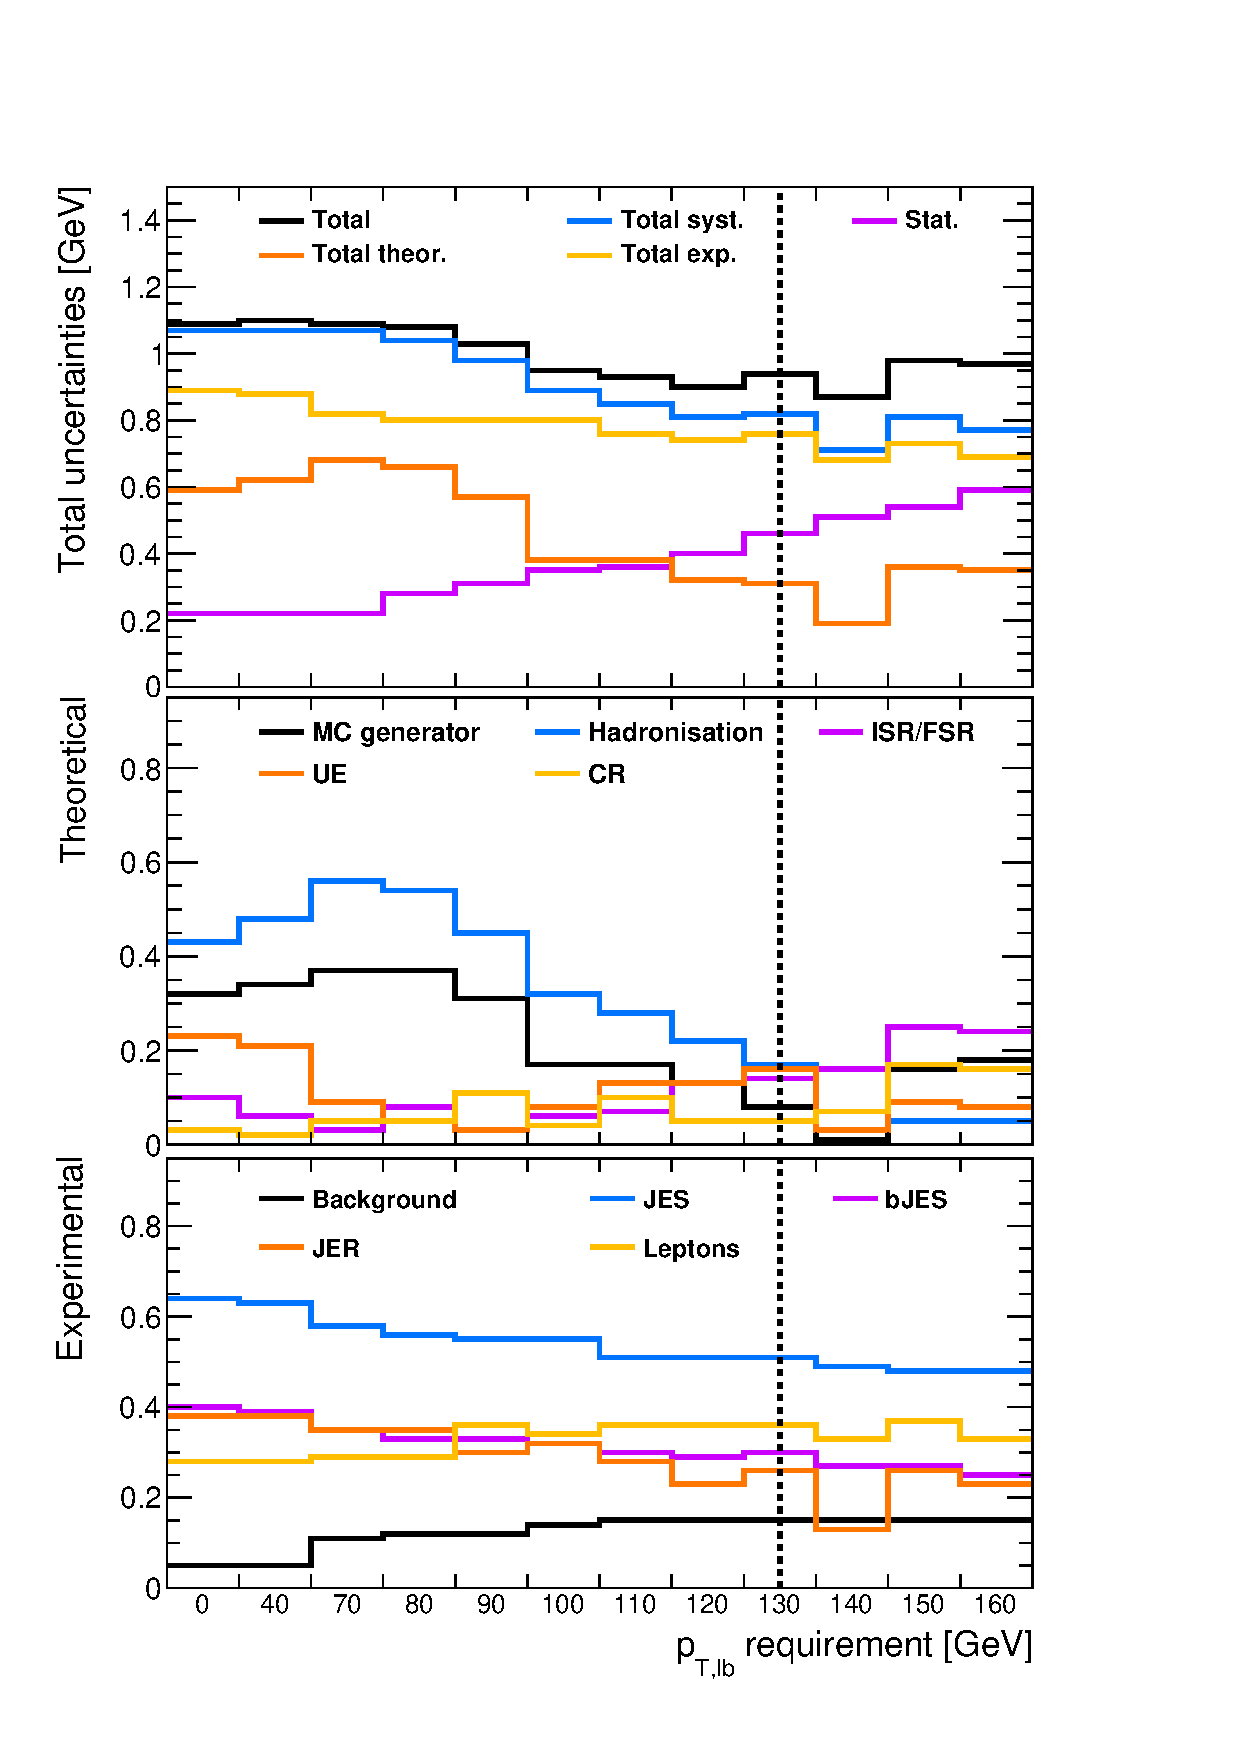
\includegraphics[width=0.49\textwidth]{./figs/fig_8TeV_TRC28_wp70/mlb_sel3_optimization_profile_ptlb.pdf}
  \label{sfig:ptlb_optimisation}
}
\subfloat[\Mvabased]{
  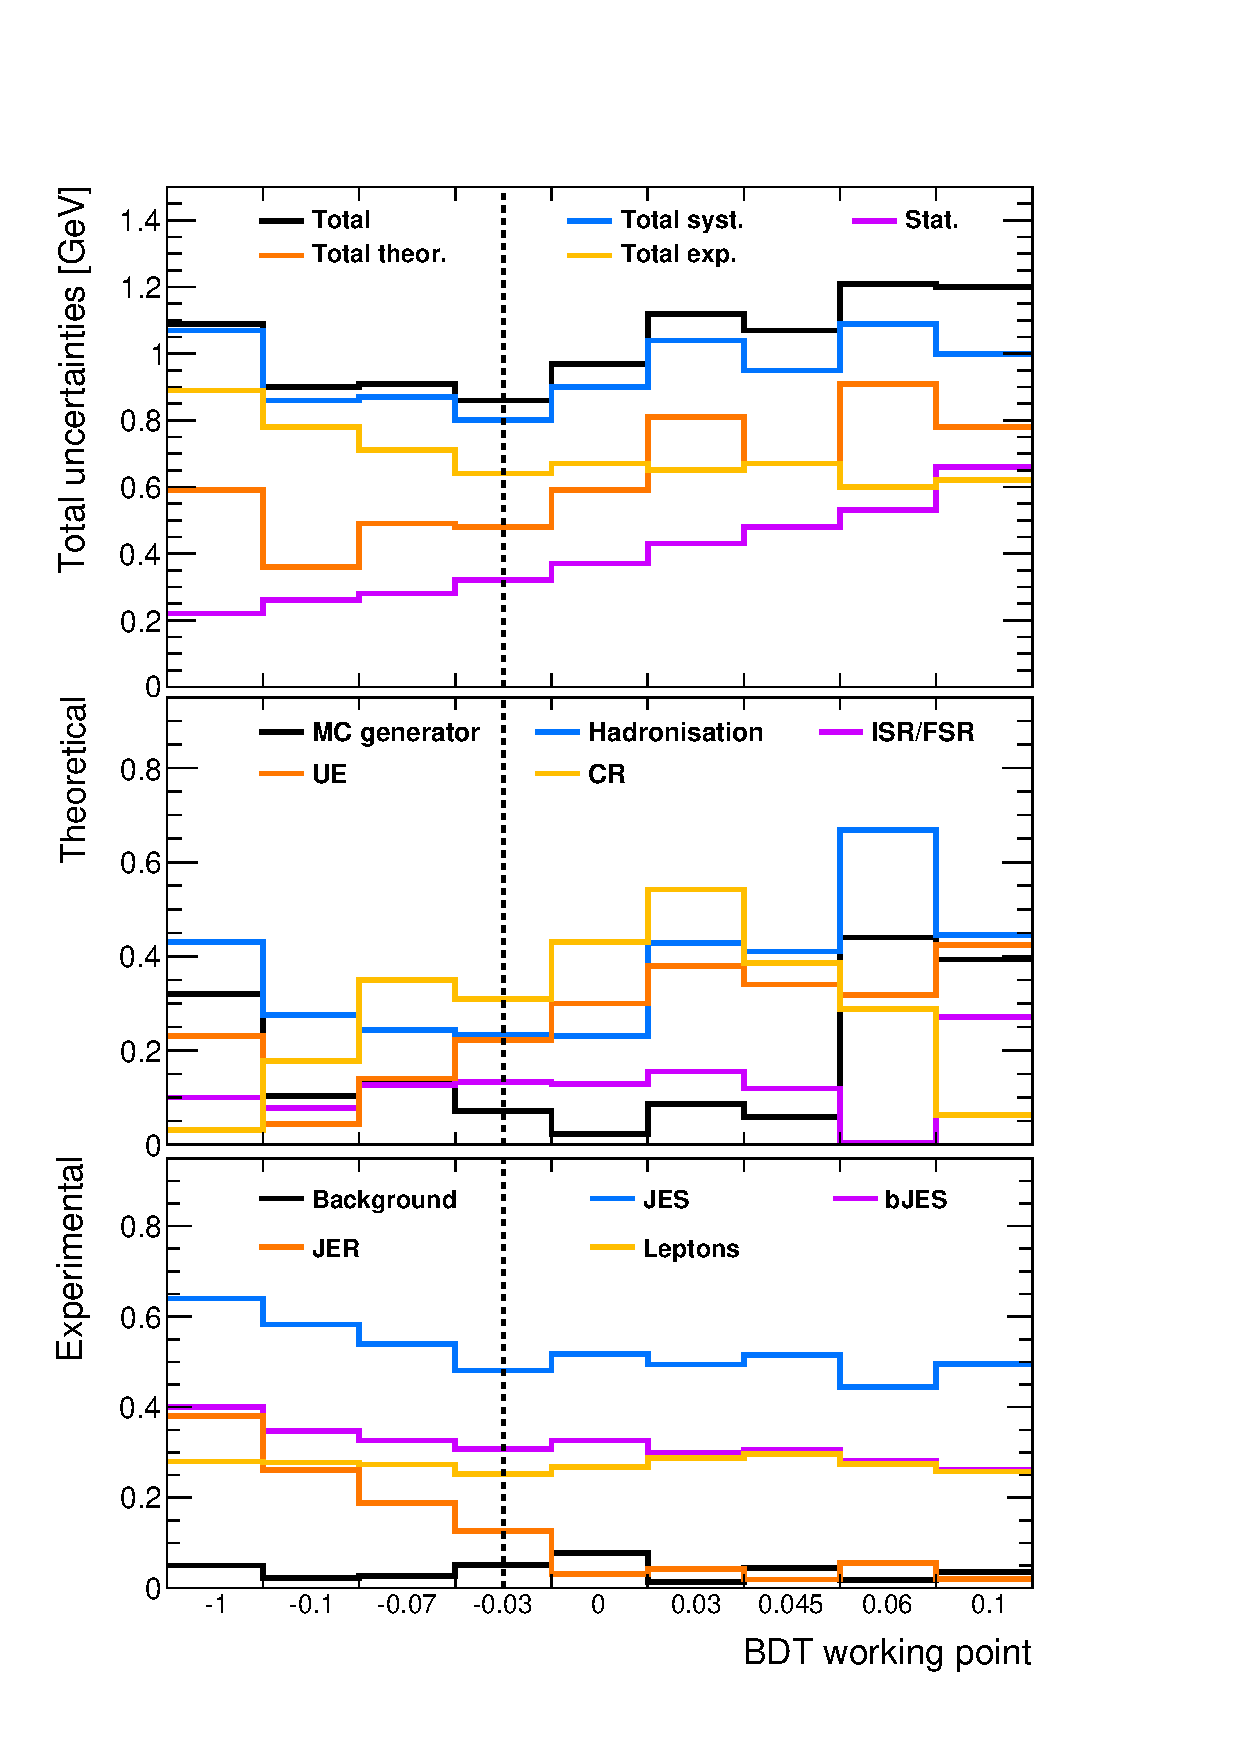
\includegraphics[width=0.49\textwidth]{./figs/fig_8TeV_TRC28_wp70/mlb_sel3_optimization_profile_BDT.pdf}
  \label{sfig:BDT_optimisation}
}
\caption[Phase space optimisation for $\sqrts=8$~\TeV\ data]{
%
The statistical and systematic uncertainties as functions of an additional \ptlb\ requirement~\subref{sfig:ptlb_optimisation} and the \gls{BDT} working point~\subref{sfig:BDT_optimisation}, applied in addition to the standard event selection. The total uncertainties are shown in the top, the theoretical in the middle and the experimental in the bottom figures. The chosen working points are indicated by the black dashed lines.
%
\label{fig:llopti}
}
\end{figure*}
%%%%%%%%%%%%%%%%%%%%%%%%%%%%%%%%%%%%%%%%%%%%%%%%%%%%%%%%%%%%%%%%%%%%%%%%%%%%%%%%%%%%%%
%

Both optimisation procedures lead to one additional event selection requirement on top of the standard selection. To determine the best performing working points for the respective procedure, the total uncertainty profile in dependence of the discriminative variable has been scanned.
%
The event selection changes have been propagated through the full analysis, including the recreation of templates and the determination of the systematic uncertainties. This is shown for the \cutbased\ and the \mvabased\ event selections in \fig~\ref{fig:llopti}, with the leftmost bin in each figure referring to the standard selection. Additional event selection requirements reduce the final number of events, which is reflected in the rising statistical uncertainty. Systematic uncertainties are subject to multiple effects and their profiles are discussed in \sect~\ref{sect:unc8TeV}.
%
An exploitation of those is the goal of the optimisation. For both methods, the chosen values of the additional requirement are indicated by the dashed lines.
%
The \cutbased\ and the \mvabased\ event selections are discussed in the following sections.
%
\Tab~\ref{tab:selections} shows the observed and predicted numbers of events at an input $\mt=172.5$~\GeV\ for the standard, the \cutbased\ and the \gls{BDT} event selections. In all cases, the observed numbers of events are in good agreement with the sum of the signal and background estimates.
% 
The respective matching performances are reported as well.
% 
%%%%%%%%%%%%%%%%%%%%%%%%%%%%%%%%%%%%%%%%%%%%%%%%%%%%%%%%%%%%%%%%%%%%%%%%%%%%%%%
\begin{table}[tb!]
\begin{center}
\small
\begin{tabular}{|l|rr|rr|rr|}
\hline
Selection & \multicolumn{2}{c|}{Standard} & \multicolumn{2}{c|}{\Cutbased} & \multicolumn{2}{c|}{\Mvabased}\\  
\hline
\ttbar\ signal            & 33500 $\pm$ & 2800 & 7800 $\pm$ &  640 & 15800 $\pm$ & 1300 \\
Single  \tquark\ (signal) &  1477 $\pm$ &   89 &  287 $\pm$ &   17 &   376 $\pm$ &   23 \\
\fake{s}                  &   230 $\pm$ &  230 &   19 $\pm$ &   19 &    73 $\pm$ &   73 \\
\Zj\                      &   165 $\pm$ &   63 & 16.4 $\pm$ &  6.9 &  23.5 $\pm$ &  9.2 \\
$WW/WZ/ZZ$                &    44 $\pm$ &   16 &  8.0 $\pm$ &  3.0 &   6.0 $\pm$ &  2.1 \\
Signal+background         & 35400 $\pm$ & 2800 & 8100 $\pm$ &  640 & 16200 $\pm$ & 1300 \\ \hline
Data                      & \multicolumn{2}{c|}{35099} 
                          & \multicolumn{2}{c|}{7346}
                          & \multicolumn{2}{c|}{16117} \\ 
\hline
Exp. bkg. frac.           & 0.01  $\pm$ & 0.01 & \bkgfrEightTeV $\pm$ & \bkgfrEightTeVunc & \bkgfrBDT $\pm$ & \bkgfrBDTunc \\
Data/MC                   & 0.99  $\pm$ & 0.08 & 0.91 $\pm$ & 0.07                        & 0.99 $\pm$ & 0.08              \\ 
\hline
Matching efficiency $\epsilon$ [\%]    & \eff $\pm$ & \effunc
													  & \Cutmatcheff   $\pm$ & \Cutmatcheffunc
													  & \BDTmatcheff   $\pm$ & \BDTmatcheffunc \\
\SelPurity\ $\pi$ [\%]    & \fracmatch $\pm$ & \fracmatchunc
													  & \Cutsignalpurity   $\pm$ & \Cutsignalpurityunc
													  & \BDTsignalpurity   $\pm$ & \BDTsignalpurityunc \\
Unmatched events [\%]       & \fracunmatch $\pm$ & \fracunmatchunc
													  & \fracunmatchopti $\pm$ & \fracunmatchoptiunc
													  & \BDTfracunmatch $\pm$ & \BDTfracunmatchunc \\
Wrongly matched events [\%] & \fracwrong $\pm$ & \fracwrongunc
													  & \fracwrongopti $\pm$ & \fracwrongoptiunc
													  & \BDTfracwrong $\pm$ & \BDTfracwrongunc \\
\hline
\end{tabular}
\end{center}
\caption[Event yields for $\sqrts=8$~\TeV\ data: optimised event selections]{
%
The observed numbers of events in the \dil\ final states in $\intlumi=\atlumo$~\invfb\ of $\sqrt{s} = 8$~\TeV\ data after the different event selections.
%
In addition, the expected numbers of signal and background events corresponding to the integrated luminosity of the data are given.
%
Two significant digits are used for the uncertainties of the predictions.
% 
Values smaller than $0.005$ are listed as $0.00$.
%
The lower rows report the matching performance with statistical uncertainties only. 
\label{tab:selections}
}
\end{table}
%%%%%%%%%%%%%%%%%%%%%%%%%%%%%%%%%%%%%%%%%%%%%%%%%%%%%%%%%%%%%%%%%%%%%%%%%%%%%%%




























\subsection{Optimisation via a phase space restriction}
\label{sect:evlselopticut}
%
Event kinematics and physics objects in high \pt\ regimes are typically reconstructed more accurately, as can e.g. be seen for jets at $\sqrts=7$~\TeV\ in \fig~\ref{fig:JES7TeV}. Consequently, effective discriminating variables are most likely correlated with the transverse momenta observed in the event.
%
To avoid a bias of the measurement, a small correlation with the estimator is desirable.
%
A variable, satisfying these requirements, is the average \pt\ of the lepton--\bjet\ systems, using the same jet to lepton assignment as for the \mlbr\ reconstruction.
%
Increasing lower limits for the \ptlb\ variable moves the bulk of the observed \ttbar\ events towards higher \pt\ regimes. 
%
As shown in \fig~\ref{fig:mlb_ptlb_corr}, the correlation coefficients of the \mlbr\ and \ptlb\ variables in the data and \gls{MC} are concordantly found to be $\rho=0.11$. 


% %
%%%%%%%%%%%%%%%%%%%%%%%%%%%%%%%%%%%%%%%%%%%%%%%%%%%%%%%%%%%%%%%%%%%%%%%%%%%%%%%%%%%%%%
\begin{figure*}[tbp!]
\centering
\subfloat[Correlation in data]{
  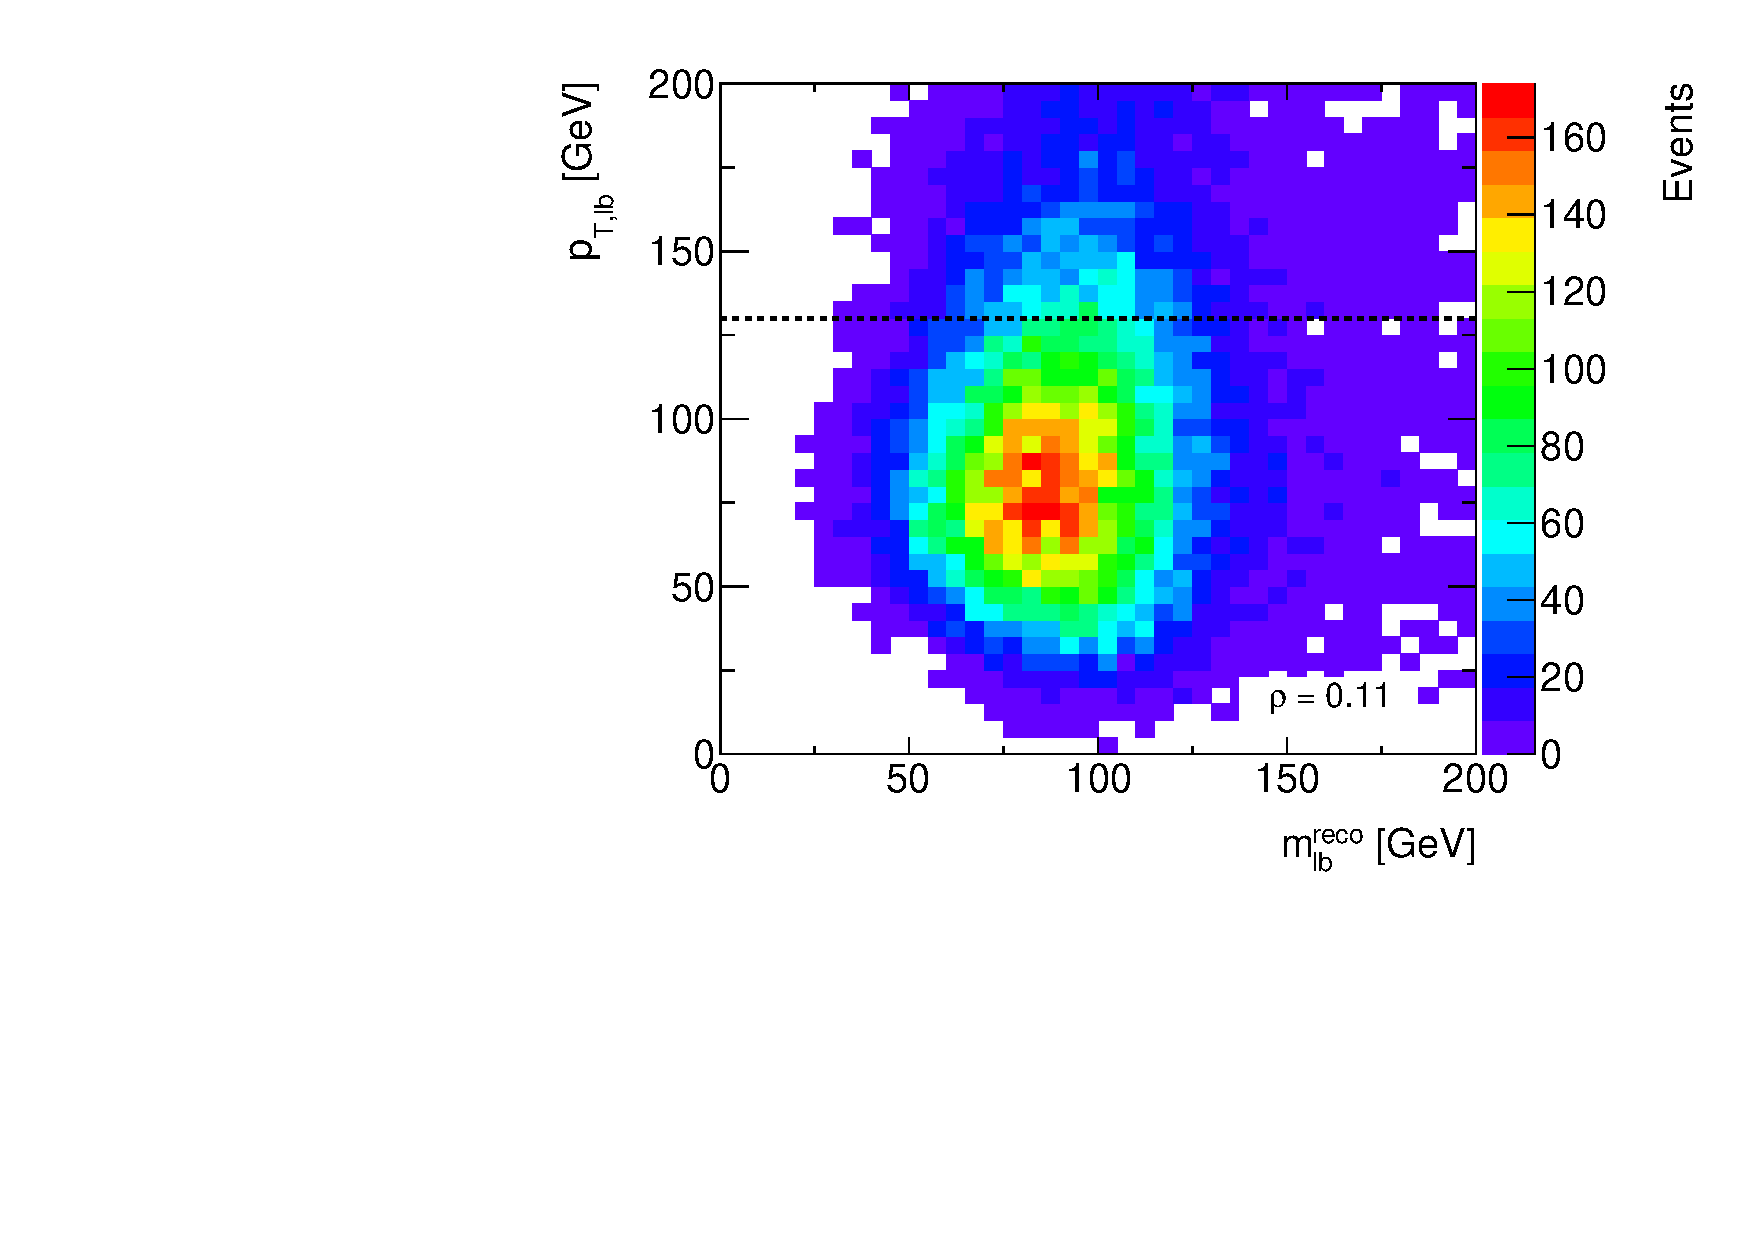
\includegraphics[width=0.49\textwidth]{./figs/fig_8TeV_TRC28_wp70/Dilep_Plot_Analysis_f1_corr_mlb_ptlb.pdf}
  \label{sfig:mlb_ptlb_corr_data}
}
\subfloat[Correlation in \gls{MC}]{
  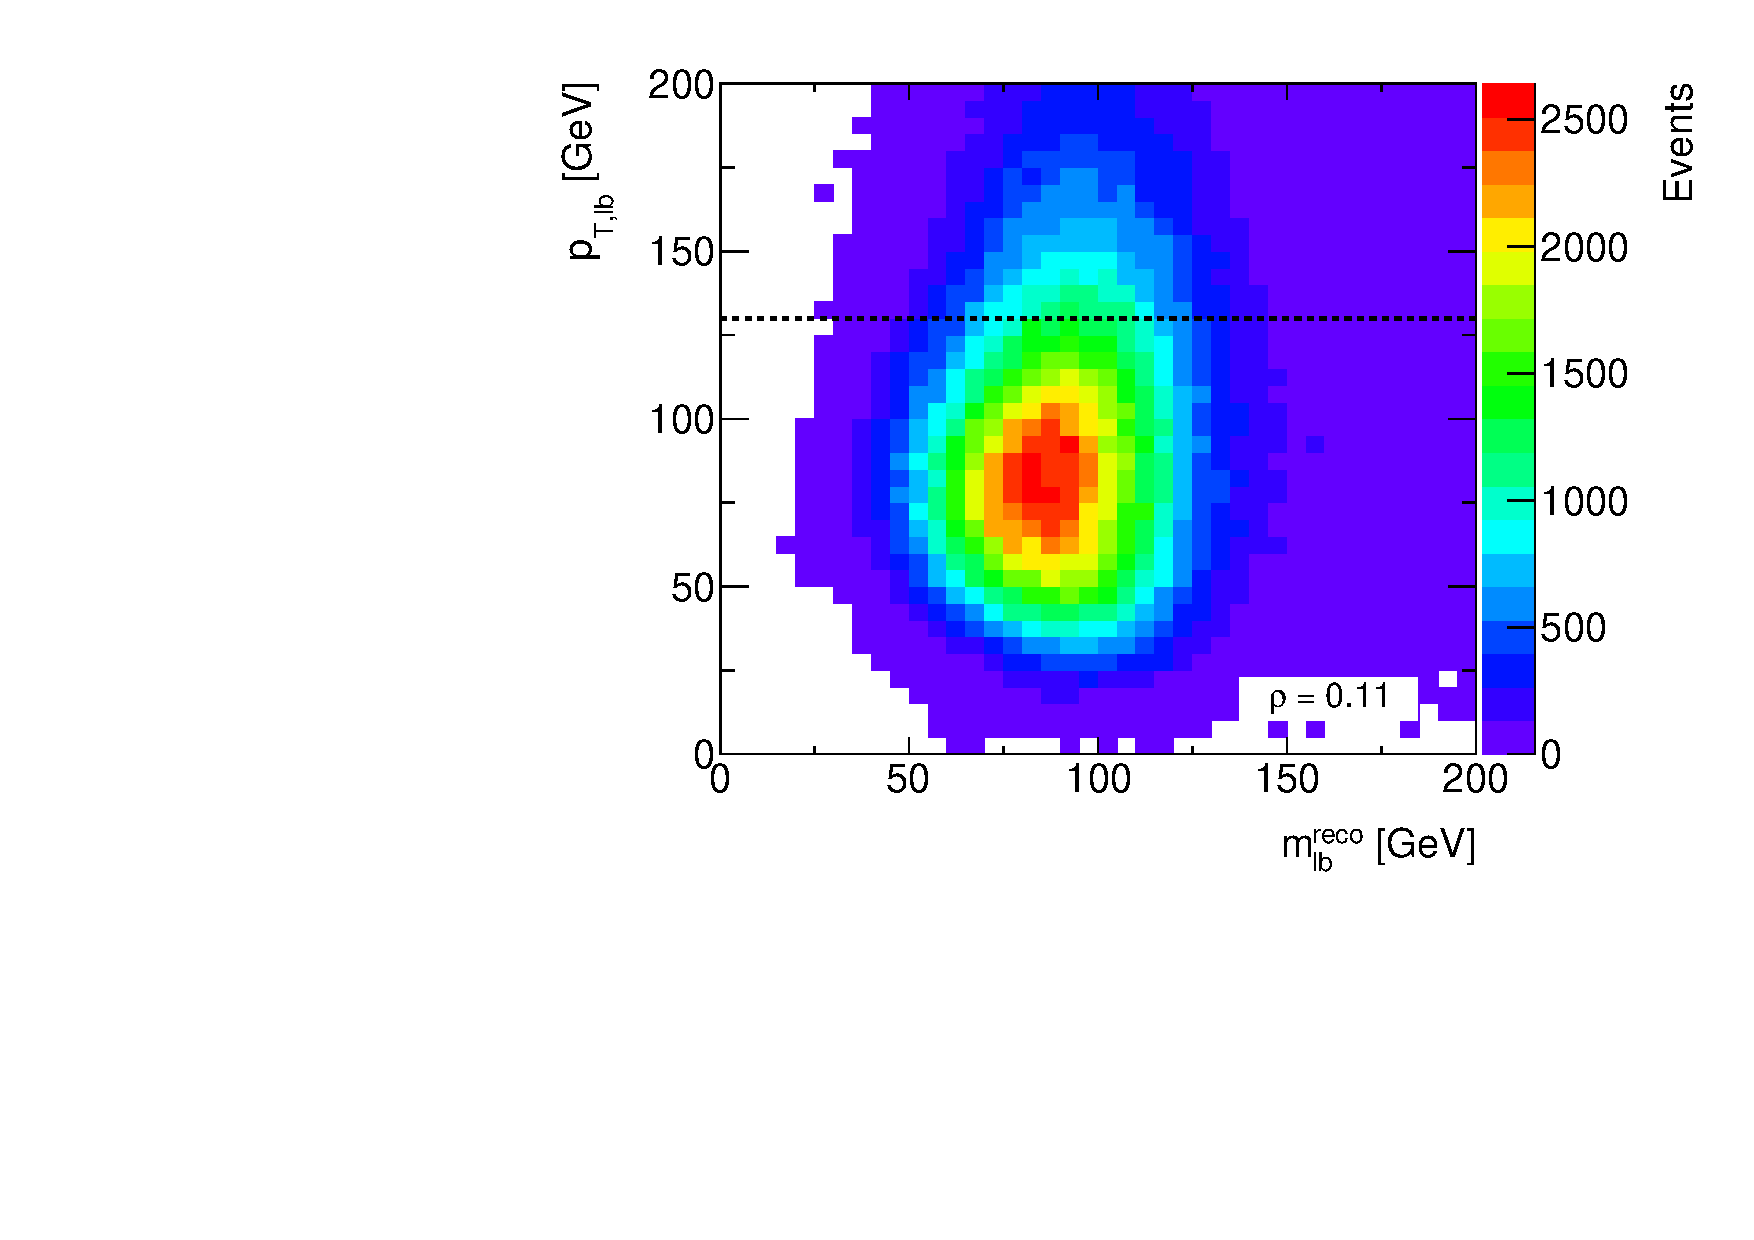
\includegraphics[width=0.49\textwidth]{./figs/fig_8TeV_TRC28_wp70/Dilep_Plot_Analysis_f172_corr_mlb_ptlb.pdf}
  \label{sfig:mlb_ptlb_corr_MC}
}
\caption[Correlation of \mlbr\ and \ptlb]{
%
% \Fig~\subref{sfig:mlb_ptlb_corr} shows the correlation of the estimator \mlbr\ with the \ptlb\ variable, used for the event selection optimisation.
The correlation of the estimator \mlbr\ with the \ptlb\ variable, used for the \cutbased\ event selection optimisation, in the data and \gls{MC}. 
%
The figures correspond to $\intlumi=\atlumo$ and about $360~\invfb$ for the data and \gls{MC}, respectively.
%
The selected phase space corresponds to the area above the black dashed line.
%
\label{fig:mlb_ptlb_corr}
}
\end{figure*}
%%%%%%%%%%%%%%%%%%%%%%%%%%%%%%%%%%%%%%%%%%%%%%%%%%%%%%%%%%%%%%%%%%%%%%%%%%%%%%%%%%%%%%
%
The dependence of the leading uncertainty components on the \ptlb\ requirement is shown in \fig~\subref*{sfig:ptlb_optimisation}.
%
The minimum total uncertainty value lies on a plateau centred around $\ptlb>130~\GeV$. 
%
This \ptlb\ condition is therefore taken as additional requirement for the \cutbased\ event selection. 
%
A similar phase space scan has been performed using a minimum requirement on the \btagged\ jet \pt,  but found to be inferior in terms of correlation to \mlb\ ($\rho=0.19$) and minimal total uncertainty ($\sigma_\mathrm{tot}^\mathrm{min}=1.01$~\GeV). 
%
With the \ptlb\ requirement, a drastic reduction in the hadronisation uncertainty is observed, accompanied by a moderate reduction in the leading two uncertainties, namely the \gls{JES} and the \gls{bJES} uncertainty. 
%
This goes along with a rising fraction of correct \bjet\ to parton matchings, compared to the standard selection. 
%
The matching performance and the reduced number of events in comparison to the standard selection are detailed in \tab~\ref{tab:selections}. The total number of data events is reduced to \OptiFraction\ of the standard event yield, with the bulk of the distribution cut out. The \gls{MC} prediction of the total yield overestimates the observation in the data by \DLevtexcopti, but it is still consistent within uncertainties. 
%
% However, this only affects the total predicted event yield and not distribution shapes, as can be verified by investigating kinematic distributions normalised to data. The template method is insensitive to total yield differences, but for a possible misdetermination of the background fraction. 
The effect on this analysis with vanishing background fraction is negligible and covered by the background normalisation uncertainties, discussed in \sect~\ref{sect:unc8TeV}.


% Distributions of several kinematic variables for the data and \gls{MC} prediction with $\mt=172.5$~\GeV\ corresponding to the \cutbased\ event selection are shown in \sect~\ref{sect:distr}, together with the distributions of the other event selections.























\subsection{Optimisation via a multivariate analysis}
\label{sect:evlselbdt}
%
The \cutbased\ optimisation procedure, using a single discriminative variable, can be improved upon by the usage of an \gls{MVA} technique. Multivariate techniques combine the discriminative power of several variables into a single discriminator of the desired category, referred to as signal, and the category to be suppressed, referred to as background. The method chosen here is the \gls{BDT} method, as implemented in the \TMVA\ package~\cite{Hocker:2007ht}, which is used in version \TMVA~4.2.0 together with \Root~5.34.25.


A decision tree consists of a set of requirements for its discriminative variables. The input events successively pass a binary decision at each node to be signal- or background-like. The order of the decisive variables and the decision limit at each node is optimised for best signal efficiency. Finally, after a specified number of splits, referred to as tree depth, each event ends up in a signal or background leaf. This is the start point for a second tree, reprocessing the misidentified events from the first tree. This is done by assigning additional weight to them in the selection, referred to as boost. This procedure is repeated until a forest of trees is obtained. A weighted average of the tree decisions is then taken as the \gls{BDT} output distribution, referred to as \gls{BDT} response.
%
The boosting type used in this analysis is the adaptive boosting technique with a learning rate of $\beta=0.5$. The adaptive boosting technique performs best on discriminative variables with weak decisive power. A tree depth of 3 is chosen for a maximum of 800 decision trees. The minimum number of training events required in a node is set to 5\% of the total number of events. The node splitting algorithm uses the Gini index~\cite{Hocker:2007ht} as impurity measure to evaluate the separation gain of a given splitting. The total separation power of a variable is calculated as the number of occurrences of the variable in nodes weighted by the separation gain squared and the number of events in that node~\cite{TreeSeparation}. For the training, half of the central \ttbar\ sample at $\mt=172.5$~\GeV\ has been used, corresponding to about $\intlumi=180~\invfb$, which is nine times the data luminosity. The other half is used for evaluating the performance of the algorithm.
%on separation power of a variable http://www.biostat.jhsph.edu/~ririzarr/Teaching/649/section-11.pdf

%
The \gls{BDT} is trained to optimise the \selPurity\, starting from the standard event selection, selecting events with high probability of a correct jet to parton matching. The signal category therefore contains the $\fracmatch\%$ correctly matched events in the central \ttbar\ sample after the standard selection. The background category is defined as the rest, i.e. the sum of unmatched and wrongly matched events.
%
Starting from more than 30 promising discriminating variables, an investigation has been performed to eliminate redundant or insignificant input variables to the \gls{BDT}. 
%
For pairs of highly correlated variables, only one has been retained as input to the \gls{BDT}. 
%
The thirteen variables with a discriminative power larger than $0.2\%$ are chosen. They are given in \tab~\ref{tab:BDTvars}.
%
%%%%%%%%%%%%%%%%%%%%%%%%%%%%%%%%%%%%%%%%%%%%%%%%%%%%%%%%%%%%%%%%%%%%%%%%%%%%%%%%
\begin{table}[tbp!]
% \footnotesize
\begin{center}
\begin{tabular}{|c|c|l|}
\hline
Separation & Variable             & Comment \\ \hline
9.3\%  & $n_{b-\mathrm{jets}}$    & Number of \btagged\ jets \\
7.8\%  & $\mttwo             $    & Transverse mass of the lepton--\btagged\ jet\ systems \\
7.2\%  & $p_\mathrm{T,j_1}       $ & Second highest \btagged\ jet\ \pt\ \\
5.7\%  & $p_\mathrm{T,j_0}       $ & Highest \btagged\ jet\ \pt\ \\
4.5\%  & $p_\mathrm{T,lb}       $ & Average \pt\ of lepton--\btagged\ jet\ systems \\
1.2\%  & $\dR_\mathrm{j_0l_0}$      & \dR\ of highest \pt\ \btagged\ jet\ and highest \pt\ lepton \\
1.0\%  & $\dR_\mathrm{j_0j_1}$      & \dR\ of \btagged\ jet{s} \\
0.9\%  & $\dR_\mathrm{l_0l_1}$      & \dR\ of leptons \\
0.8\%  & $\dR_\mathrm{j_1l_0}$      & \dR\ of second highest \pt\ \btagged\ jet\ and highest \pt\ lepton \\
0.8\%  & $\dR_\mathrm{j_0l_1}$      & \dR\ of highest \pt\ \btagged\ jet\ and second highest \pt\ lepton \\
0.4\%  & $p_\mathrm{T,l_0}       $ & Highest lepton \pt\ \\
0.2\%  & $p_\mathrm{T,l_1}       $ & Second highest lepton \pt\ \\
0.2\%  & $\dR_\mathrm{j_1l_1}$      & \dR\ of second highest \pt\ \btagged\ jet\ and second highest \pt\ lepton \\ \hline
\end{tabular}
\end{center}
\caption[Input variables to the \gls{BDT}]{
%
The input variables to the \gls{BDT} ranked by their separation power.
%
\label{tab:BDTvars}
}
\end{table}
%%%%%%%%%%%%%%%%%%%%%%%%%%%%%%%%%%%%%%%%%%%%%%%%%%%%%%%%%%%%%%%%%%%%%%%%%%%%%%%%



%
%%%%%%%%%%%%%%%%%%%%%%%%%%%%%%%%%%%%%%%%%%%%%%%%%%%%%%%%%%%%%%%%%%%%%%%%%%%%%%%
\begin{figure*}[tbp!]
\centering
\subfloat[Number of \btagged\ jets]{
  % \includegraphics[width=0.49\textwidth,trim={0 150 380 0},clip]{./figs/fig_TMVA_8TeV_TRC28_wp70/variables_id_c3.eps}
  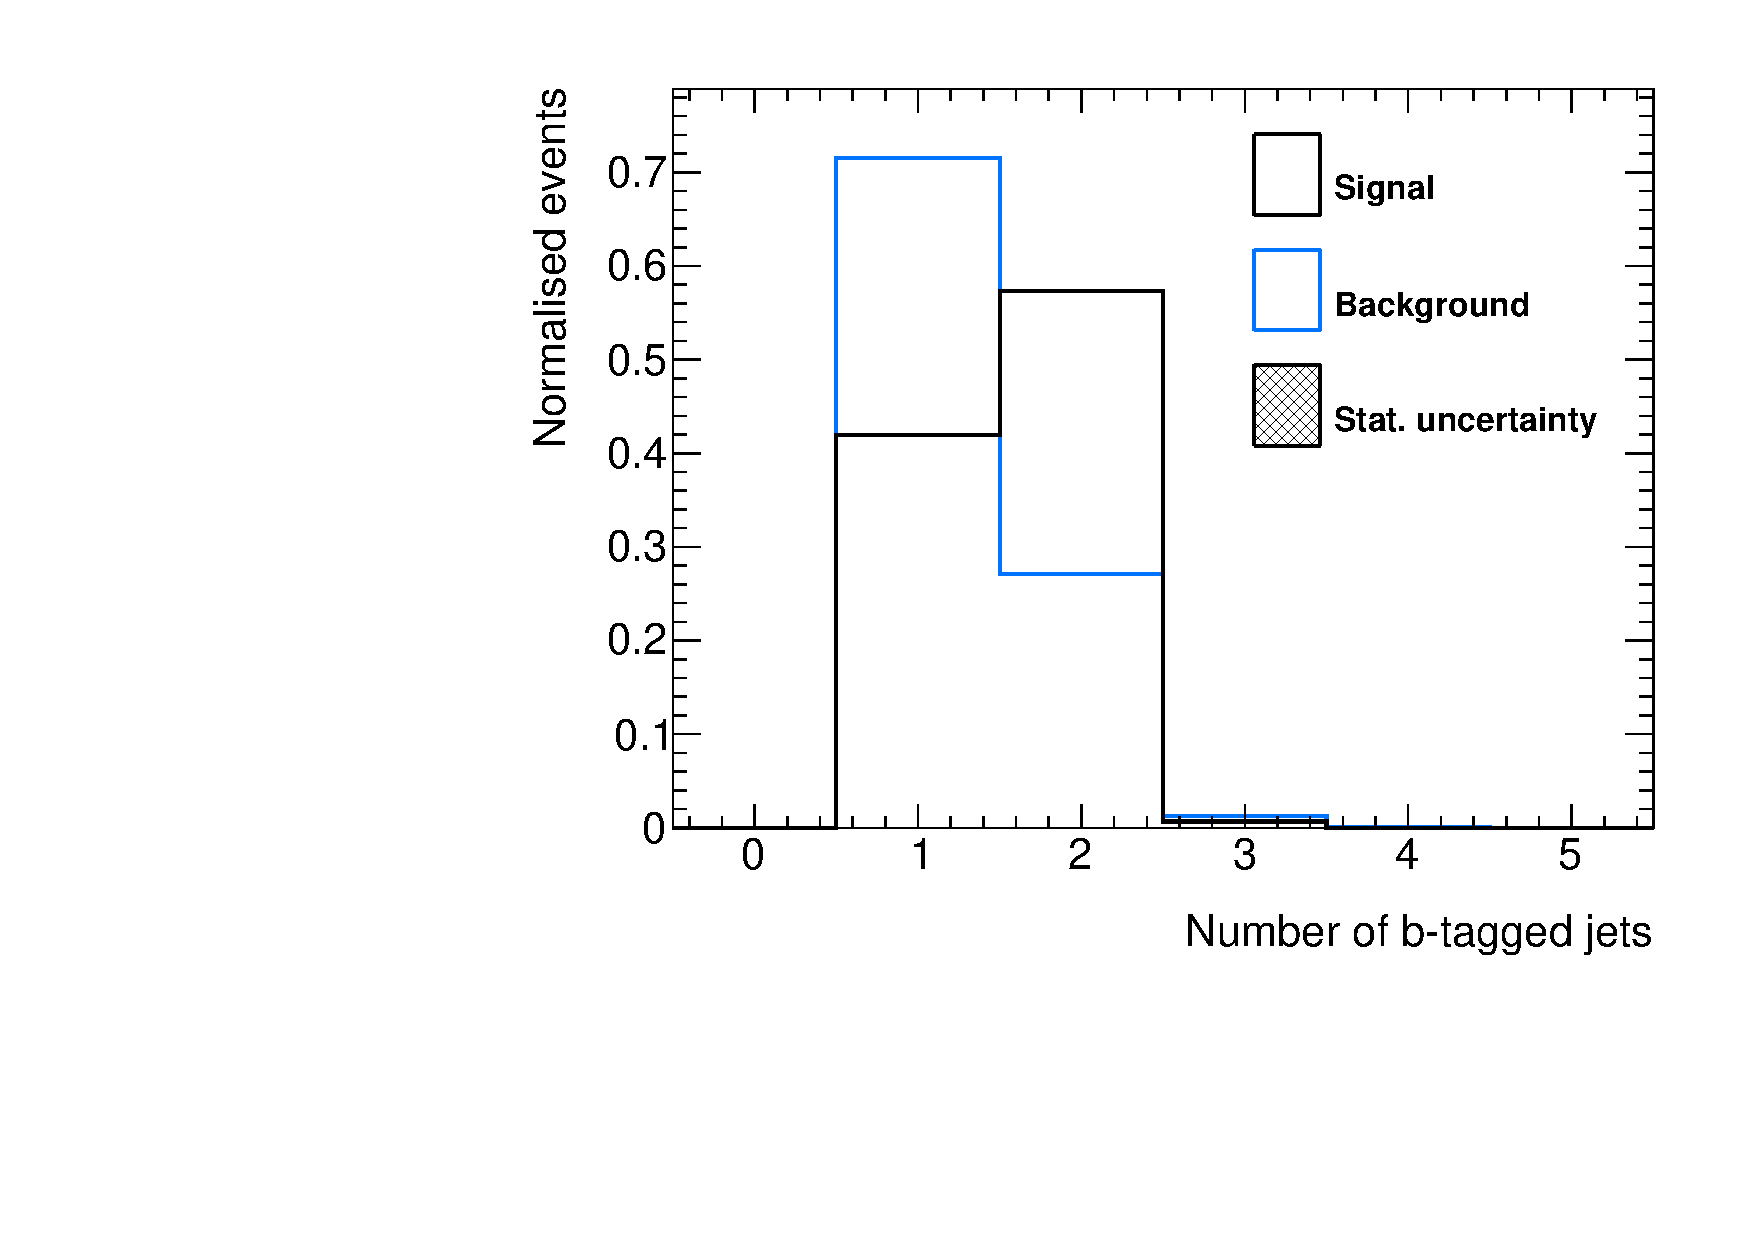
\includegraphics[width=0.49\textwidth]{./figs/fig_8TeV_TRC28_wp70_BDT-0.03/mlb_discr_bjet_n.pdf}
  \label{sfig:bdtnbjet}
}
\subfloat[\mttwo]{
  % \includegraphics[width=0.49\textwidth,trim={190 150 190 0},clip]{./figs/fig_TMVA_8TeV_TRC28_wp70/variables_id_c1.eps}
  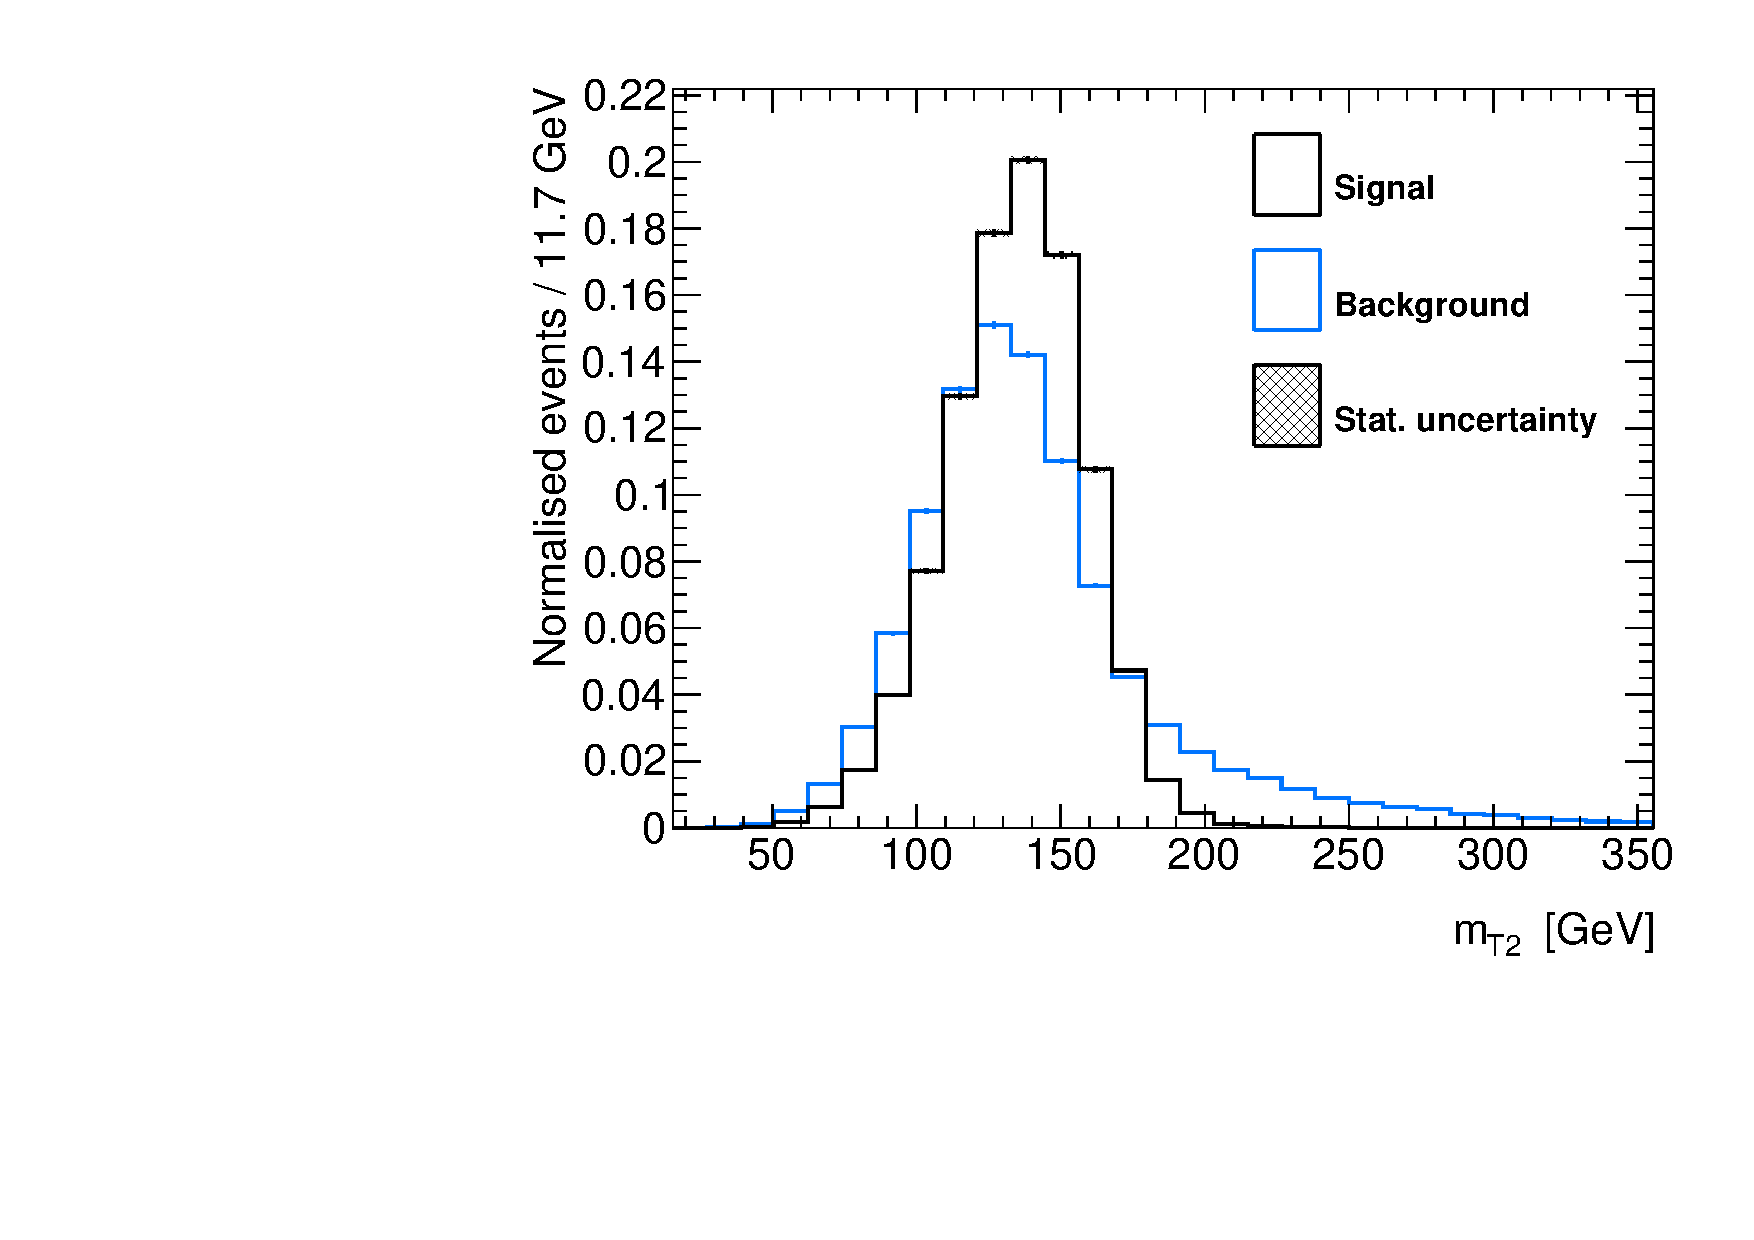
\includegraphics[width=0.49\textwidth]{./figs/fig_8TeV_TRC28_wp70_BDT-0.03/mlb_discr_mt2.pdf}
  \label{sfig:bdtmt2}
}
\hfill
\subfloat[\ptlb]{
  % \includegraphics[width=0.49\textwidth,trim={0 150 380 0},clip]{./figs/fig_TMVA_8TeV_TRC28_wp70/variables_id_c1.eps}
  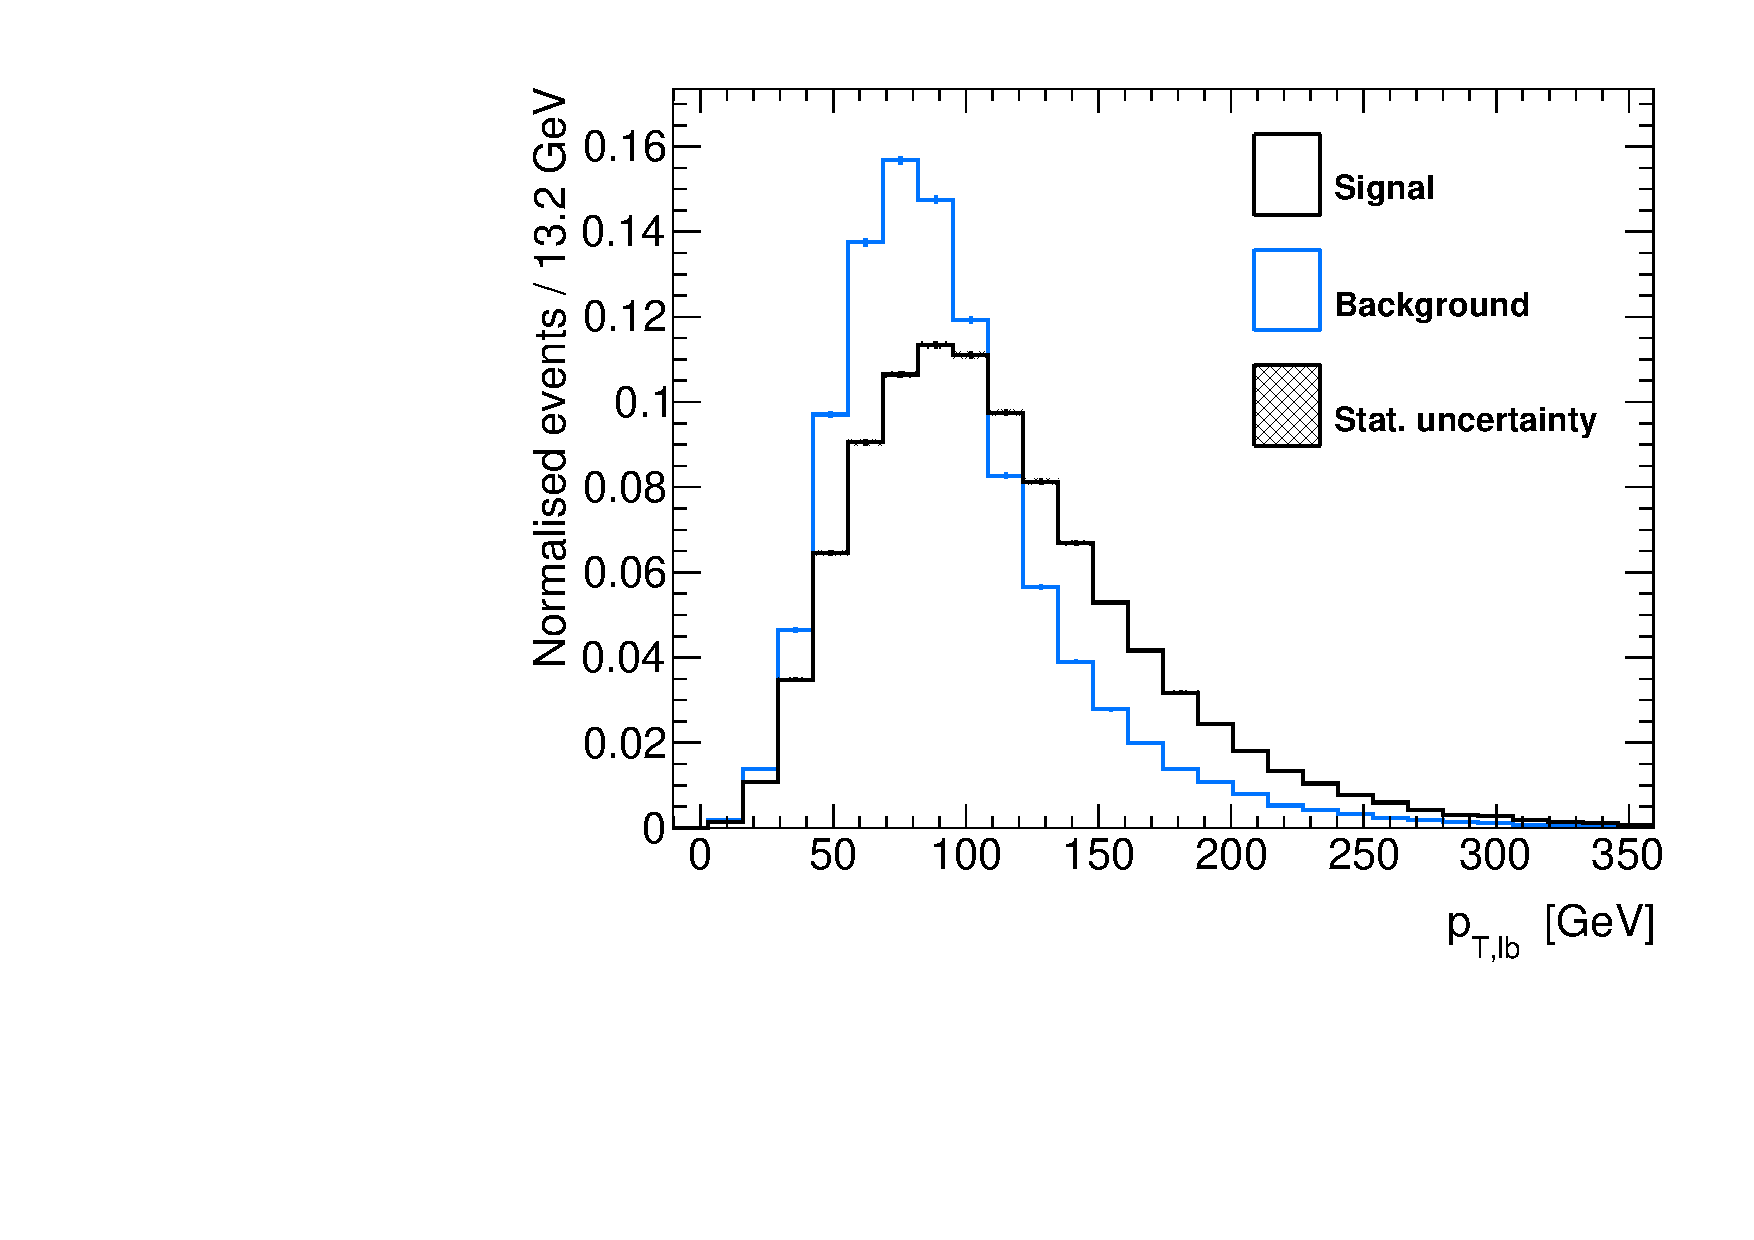
\includegraphics[width=0.49\textwidth]{./figs/fig_8TeV_TRC28_wp70_BDT-0.03/mlb_discr_ptlb.pdf}
  \label{sfig:bdtptlb}
}
\subfloat[$\dR_\mathrm{j_0l_0}$]{
  % \includegraphics[width=0.49\textwidth,trim={190 150 190 0},clip]{./figs/fig_TMVA_8TeV_TRC28_wp70/variables_id_c2.eps}
  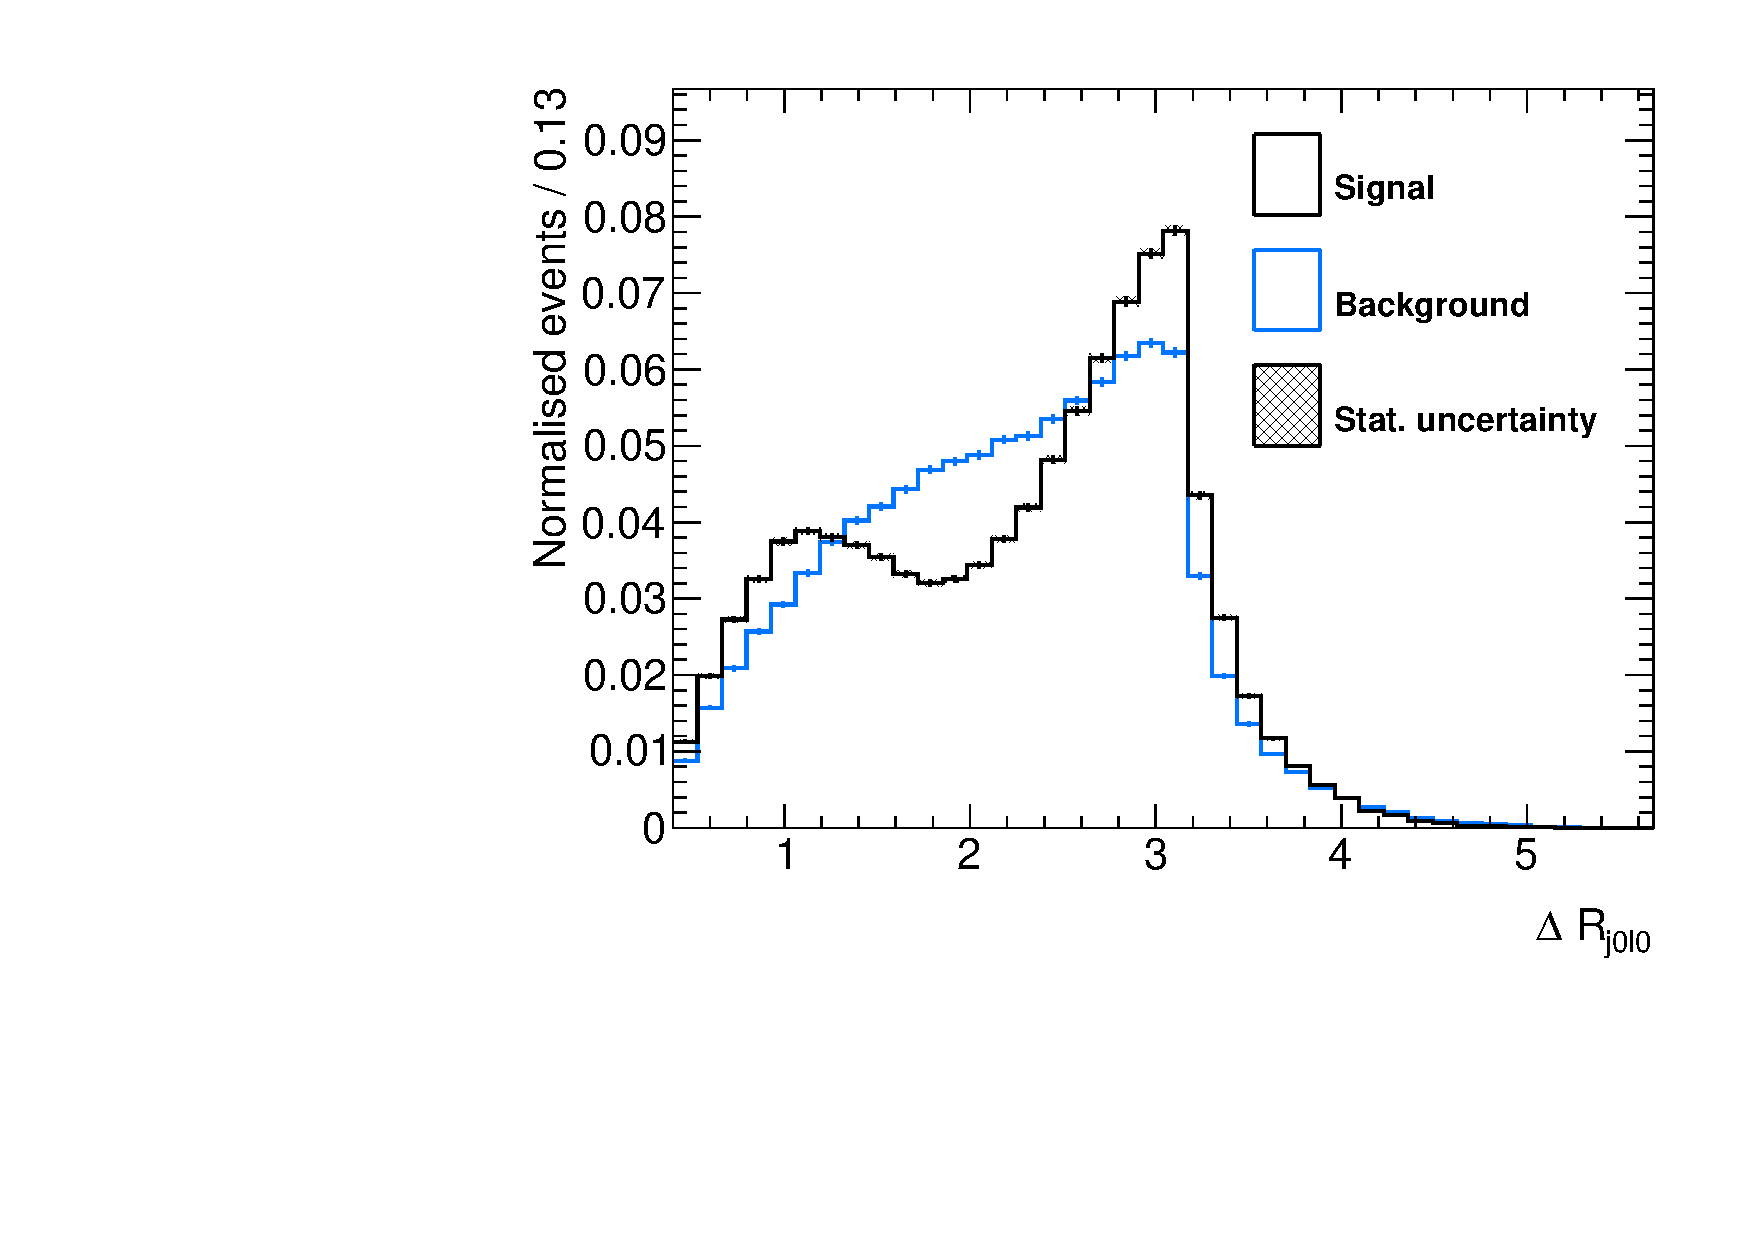
\includegraphics[width=0.49\textwidth]{./figs/fig_8TeV_TRC28_wp70_BDT-0.03/mlb_discr_dRj0l0.pdf}
  \label{sfig:bdtdRj0l0}
}
\hfill
\subfloat[\gls{BDT} response for signal and background]{
  % \includegraphics[width=0.49\textwidth]{./figs/fig_TMVA_8TeV_TRC28_wp70/mva_BDT.eps}
  % \includegraphics[width=0.49\textwidth]{./figs/fig_TMVA_8TeV_TRC28_wp70/overtrain_BDT.eps}
  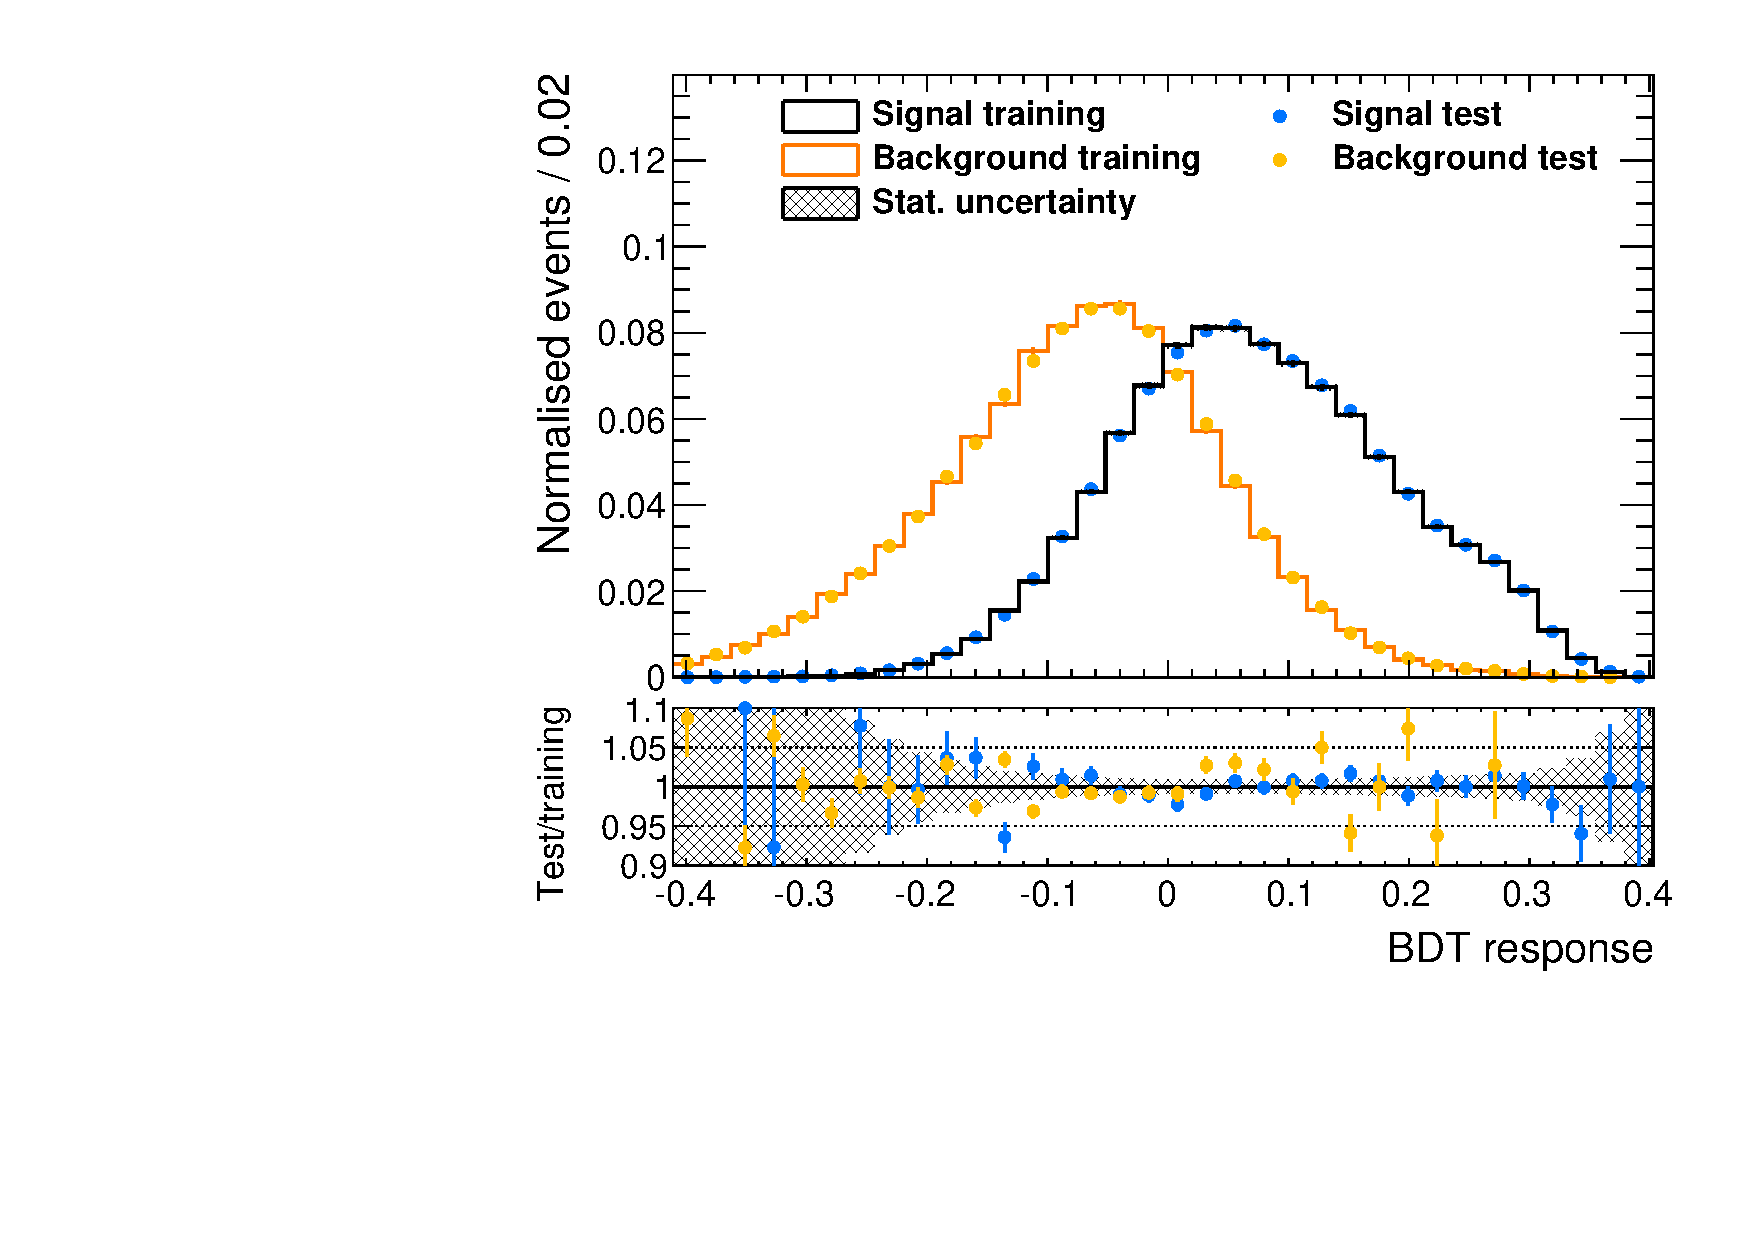
\includegraphics[width=0.49\textwidth]{./figs/fig_8TeV_TRC28_wp70_BDT-0.03/mlb_discr_response.pdf}
  \label{sfig:bdtmva_BDT}
}
\subfloat[\gls{BDT} response in data and \gls{MC}]{
  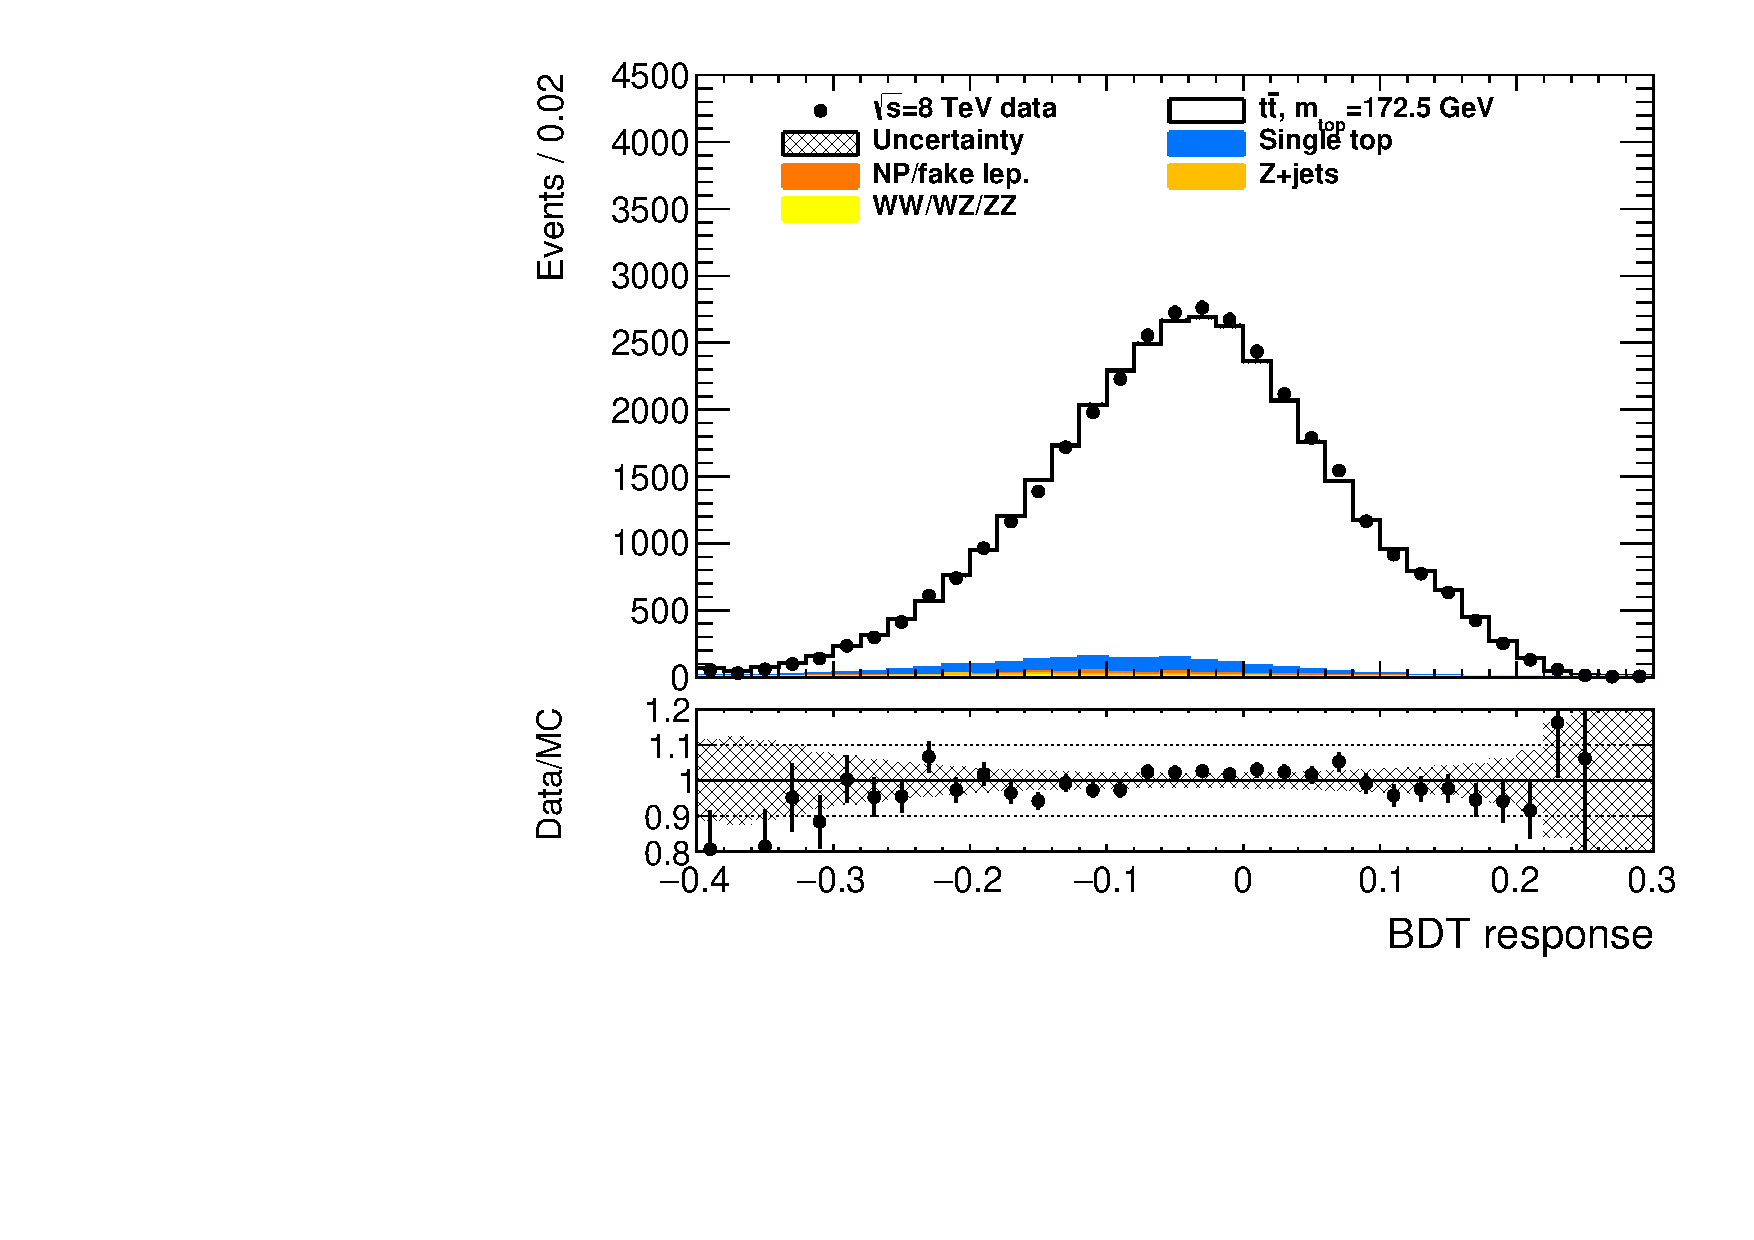
\includegraphics[width=0.49\textwidth]{./figs/fig_8TeV_TRC28_wp70/Dilep_SgnBkg_ratio_norm_sel3_BDT_response.pdf}
  \label{sfig:bdtmva_BDT_data}
}
%
\caption[Input variables and response of the \gls{BDT}]{
%
Examples of input variables and response of the \gls{BDT}.
%
The \fig{s}~\subref{sfig:bdtnbjet} to \subref{sfig:bdtdRj0l0} show the normalised signal and background distributions for the number of \btagged\ jets, the \mttwo\ the \ptlb\ and the \dR\ of the highest \pt\ \bjet\ and the highest \pt\ lepton.
%
\Fig~\subref{sfig:bdtmva_BDT} shows the final \gls{BDT} response distributions for signal and background, evaluated on the test and on the training sample.
%
The data to \gls{MC} comparison for the \gls{BDT} response is shown in \fig~\subref{sfig:bdtmva_BDT_data}, with the prediction normalised to the observed number of data events.
%
The bin sizes correspond to a total of 50 bins over the full variable range, the standard setting of the \TMVA\ software.
%
\label{fig:bdtvars}}
\end{figure*}
%%%%%%%%%%%%%%%%%%%%%%%%%%%%%%%%%%%%%%%%%%%%%%%%%%%%%%%%%%%%%%%%%%%%%%%%%%%%%
%
The normalised distributions of the leading two variables together with the \ptlb\ and the \dR\ between the highest \pt\ \btagged\ jet and the highest \pt\ lepton $\dR_\mathrm{j_0l_0}$ are shown in \fig~\ref{fig:bdtvars}, together with the final \gls{BDT} response for signal and background. 
%
The high susceptibility for a mismatch in the case of one \btagged\ jet reported in \tab~\ref{tab:stdselDL8TeV} is reflected in the deviation shown in \fig~\subref*{sfig:bdtnbjet}.
%
%
% It is generally defined as $m_\mathrm{T}^2=m_0^2+\pt^2$ and used for the partial reconstruction of decays including one or more invisible daughter particles~\cite{Barr:2003rg,Lester:1999tx,Maier2012}. 
%
The \mttwo\ variable is a transverse mass of the lepton--\bjet\ systems with a natural cut-off at the \tquark\ mass. As can be seen in \fig~\subref{sfig:bdtmt2}, the unphysical values stem predominantly from unsuccessful jet to parton matching. \Fig~\subref{sfig:bdtptlb} shows the generally lower \ptlb\ values for background events, which is in line with the observation from the \cutbased\ analysis that high \ptlb\ values favour a correct assignment. In \fig~\subref{sfig:bdtdRj0l0}, the \dR\ distribution between the leading \pt\ jet and lepton displays two peaks for correctly matched events. The low \dR\ peak corresponds to the cases where the high-\pt\ jet and lepton correspond to the same \tquark\ and the high \dR\ peak to the cases where they do not. The region in between is less populated since the \tquark\ decay products tend to be collimated. This feature is not visible in the background distribution, since the lepton--\btagged\ jet pairs do not stem from the same \tquark. \Fig~\subref{sfig:bdtmva_BDT} shows the resulting \gls{BDT} response for signal and background, evaluated on the training and on the test sample.
%
Bias by overtraining of the \gls{BDT} can be excluded from the good agreement of the \gls{BDT} response in the training and the test sample. The resulting p-values of a Kolmogorov-Smirnov test are $8\%$ and $0.2\%$ for the signal and background response distributions, respectively.
%see https://cds.cern.ch/record/1416762/files/ATL-COM-PHYS-2012-042.pdf
%
The \gls{BDT} response in \gls{MC} is in reasonable agreement with the one observed in the data, as shown in \fig~\subref{sfig:bdtmva_BDT_data}. 
%
This justifies the application of the \gls{BDT} approach to the data.


%
%%%%%%%%%%%%%%%%%%%%%%%%%%%%%%%%%%%%%%%%%%%%%%%%%%%%%%%%%%%%%%%%%%%%%%%%%%%%%%%
\begin{figure*}[tbp!]
\centering
\subfloat[Signal and background correlation matrices]{
  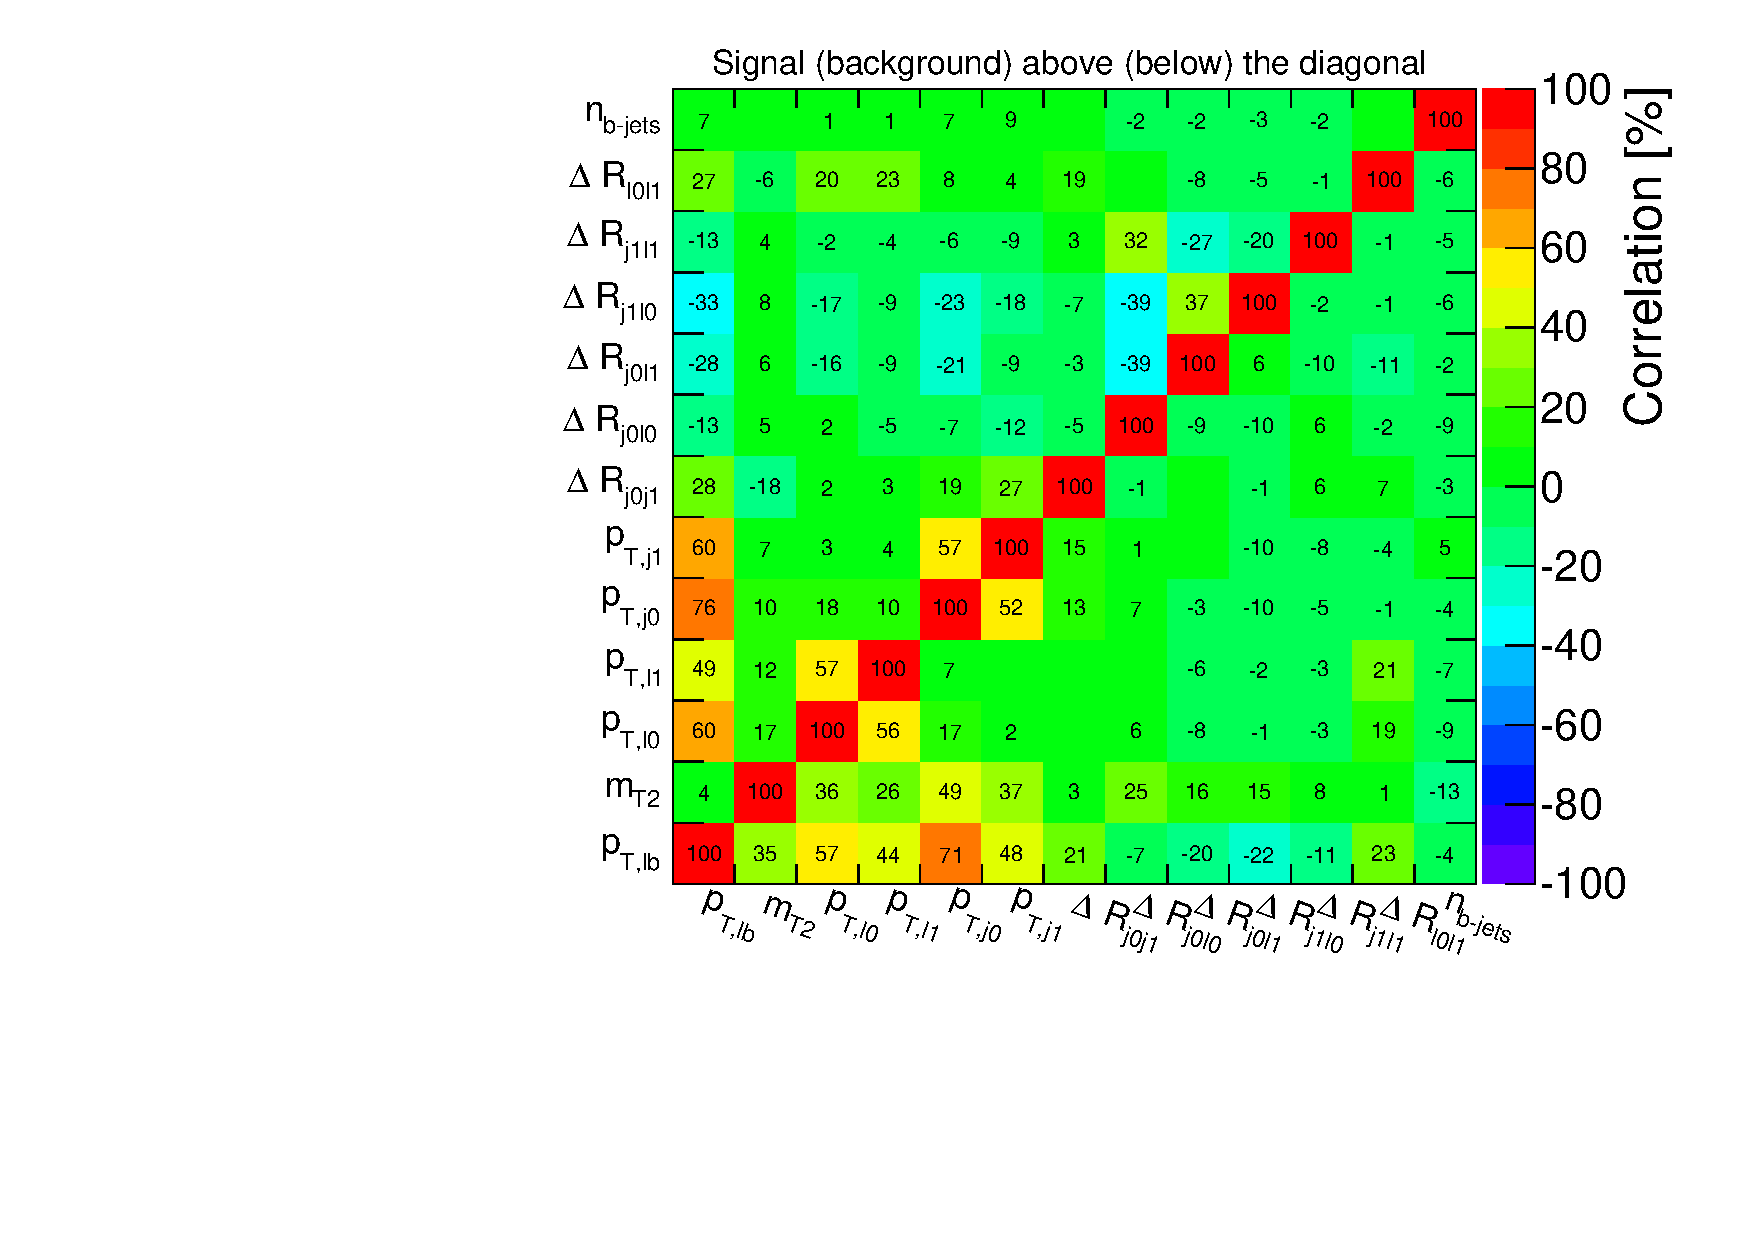
\includegraphics[width=0.49\textwidth]{./figs/fig_8TeV_TRC28_wp70_BDT-0.03/mlb_BDT_corr_sigandbkg.pdf}
  \label{sfig:bdtvarcorrSB}
}
\subfloat[Signal minus background correlation matrix]{
  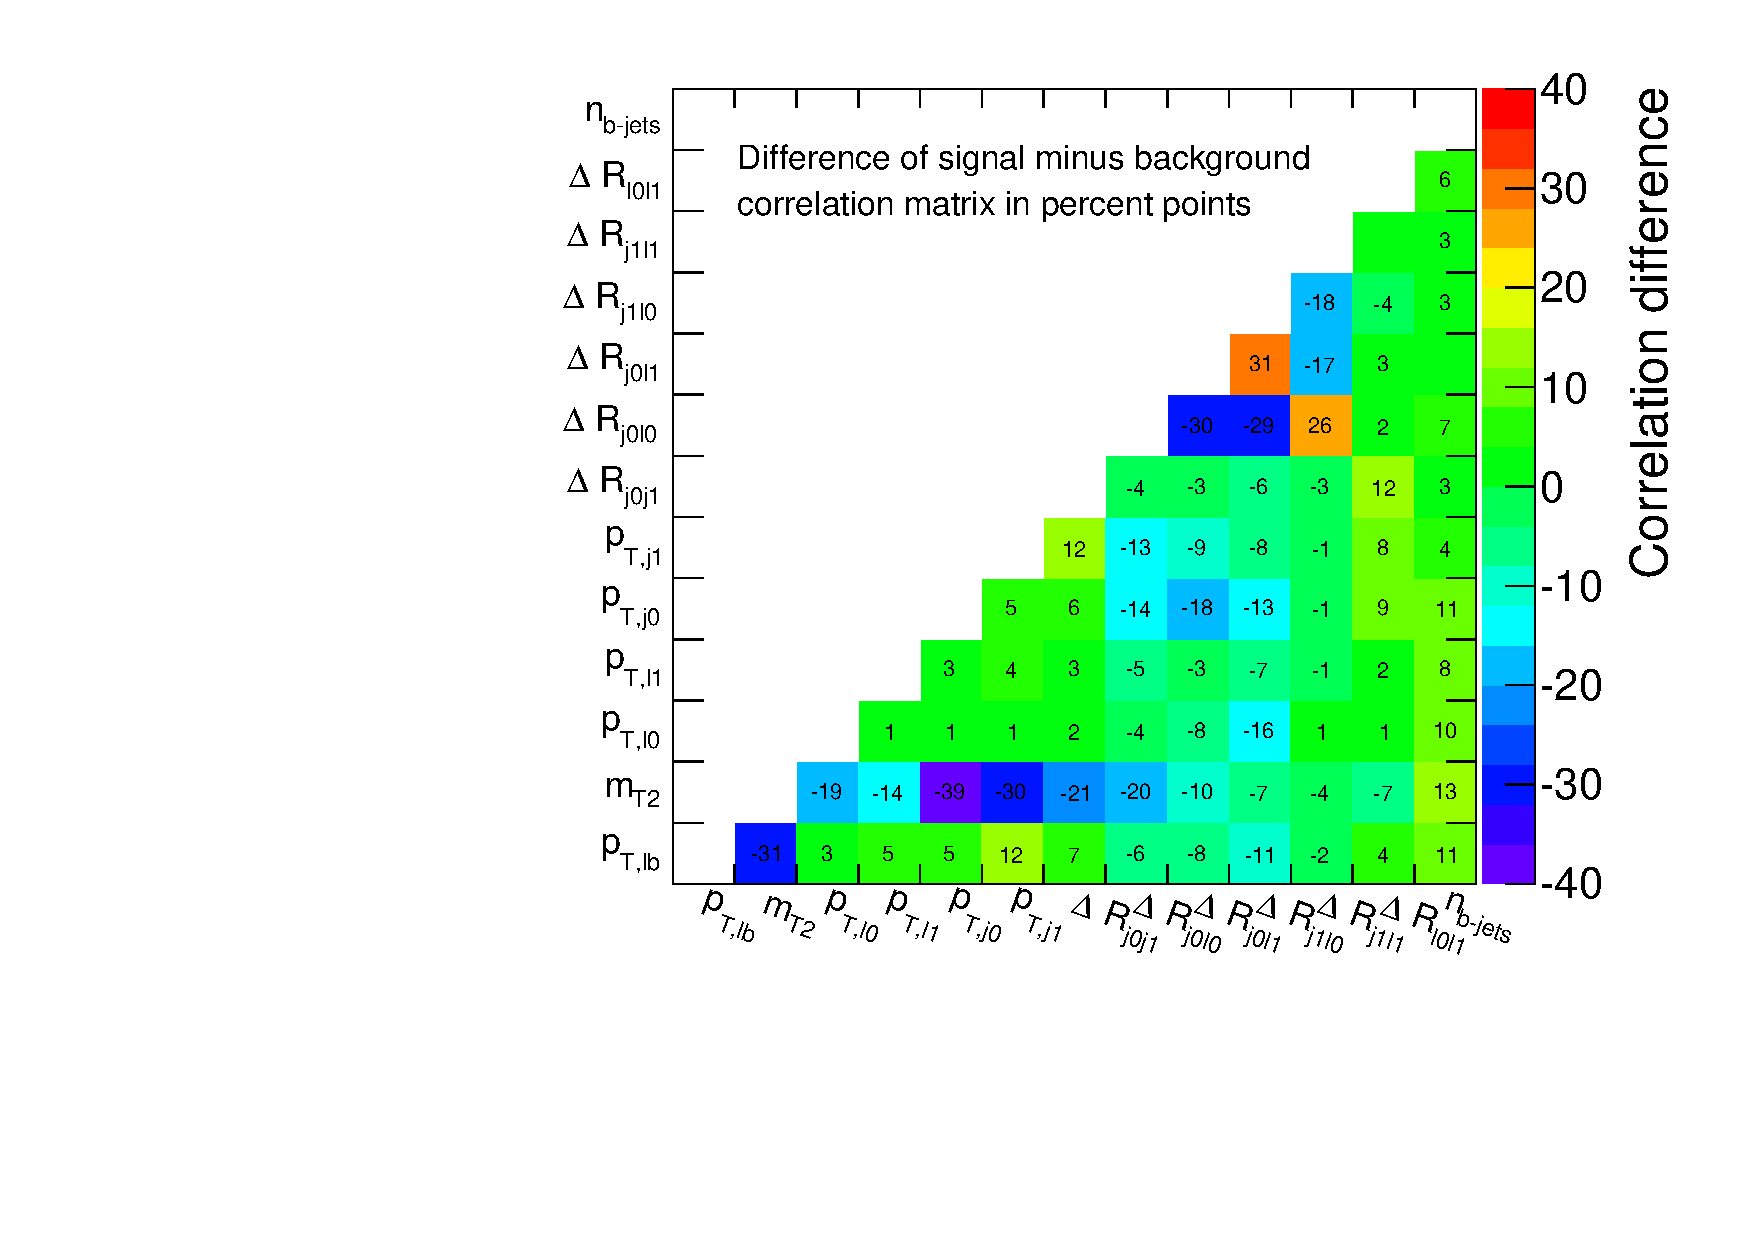
\includegraphics[width=0.49\textwidth]{./figs/fig_8TeV_TRC28_wp70_BDT-0.03/mlb_BDT_corr_diffsigbkg.pdf}
  \label{sfig:bdtvarcorrDiff}
}
%
\caption[Correlation of input variables of the \gls{BDT}]{
%
\Fig~\subref{sfig:bdtvarcorrSB} shows the correlation matrices of the input variables of the \gls{BDT} for the signal above and for the background below the diagonal. The difference of the signal minus the background correlation matrix in percent points is given in \fig~\subref{sfig:bdtvarcorrDiff}. Empty coloured bins indicate a correlation coefficient or a correlation coefficient difference of 0. 
%
\label{fig:bdtvarcorr}}
\end{figure*}
%%%%%%%%%%%%%%%%%%%%%%%%%%%%%%%%%%%%%%%%%%%%%%%%%%%%%%%%%%%%%%%%%%%%%%%%%%%%%
%
The pairwise linear correlation coefficients of the \gls{BDT} input variables are given in \fig~\subref*{sfig:bdtvarcorrSB} for signal and background, and in \fig~\subref{sfig:bdtvarcorrDiff} for the difference signal minus background. The correlation matrices are symmetric and only one side of the diagonal is shown in each case. Differences in the correlation can be exploited by the separation algorithm and the variable ranking in \tab~\ref{tab:BDTvars} is reflected in the correlations.
%
Higher correlations can be seen for variables within the same category of angular and momentum related observables and for the \ptlb\ variable, combining information from both. 
%
The dynamics leading to the correlation differences between signal and background are manifold and often not directly deducible from first principle arguments. 
%
An example is the correlation of the \pt\ of the highest and second highest \pt\ \btagged\ jets. Besides the fact that per definition $p_\mathrm{T,j0} > p_\mathrm{T,j1}$, at \gls{LO} the top and anti-\tquark\ \pt\ values balance in the event and this trend is propagated to the daughter particles. Consequently, a high-\pt\ jet in one \tquark\ decay is often balanced by a higher \pt\ jet in the other, resulting in a positive correlation. The same holds for the leptons. As expected, this feature is observed equally in the signal and background samples.
%
The \mlb\ matching algorithm, which is the basis for the signal and background classification, prefers low jet--lepton system mass and consequently low $\dR_\mathrm{j\ell}$ combinations. 
%
The positive correlation observed for the $\dR_\mathrm{j\ell}$ variables when exchanging two indices and the negative correlation when exchanging one index are consequences of the decay kinematics. 
%
% The signal sample is enriched with events where small $\dR_\mathrm{j\ell}$ is an indication for the same mother \tquark. The \tquark\ \pt\ results in a positive correlation for \dR, when exchanging both indices. Small \dR\ between the daughter particles results in large \dR\ for objects with different mother \tquark, as can also be seen in \fig~\subref*{sfig:bdtdRj0l0}. Signal events thus exhibit a pronounced \dR\ asymmetry under the exchange of one index, resulting in the negative correlation. Since the background sample does not favour small $\dR_\mathrm{j\ell}$, it does not show these features.
% %
% The largest correlation differences of signal and background are observed for the \mttwo\ variable and the number of \btagged\ jets. The consistent deviations with respect to almost many other variables indicates a different 
% \todo{why positive correlation in background and not for signal for mt2?}




Once the \gls{BDT} is successfully trained, a suitable value of the \gls{BDT} response to separate signal from background has to be found for the subsequent analysis, referred to as working point. 
%
Traditionally, the value maximising the product of signal efficiency and \selPurity\ is chosen as working point, being \BDTcutpureff\ in this case. While this purity approach may be the optimal value for a cross section analysis or a search for a hidden signal, it is not necessarily optimal for systematically limited analyses like the measurement of the \tquark\ mass. 
%
% Therefore, the working point \BDTcuteff, corresponding to the same number of final data events as observed for the \cutbased\ analysis, is also investigated. 
%
Following a similar procedure as for the \cutbased\ analysis, the minimum \gls{BDT} response value has been scanned to find the smallest total uncertainty of the analysis. The resulting profile of the leading uncertainty components is shown in \fig{s}~\subref*{sfig:BDT_optimisation}. The minimum lies at a \gls{BDT} working point of \BDTcutoptieff, driven by a reduced sensitivity to the \gls{JES} and hadronisation effects, as observed for the \cutbased\ analysis. This restriction is used as event selection requirement for the \mvabased\ selection. This requirement reduces the total number of data events to \BDTOptiFraction\ of the standard event yield.
%
Motivated by the shape of the \mlbr\ estimator distribution visible in \fig~\subref*{sfig:mlb_8TeV_mvabased}, an additional selection requirement of $50~\GeV < \mlbr < 140~\GeV$ is applied.
%



A comparison of matching performance of the different event selections is shown in the bottom rows of \tab~\ref{tab:selections}.
%
The fractions of correct \bjet\ to parton matchings are significantly improved with respect to the standard analysis. 
%
% The event selection corresponding to the \gls{BDT} working point of \BDTcutpureff\ shows a similar \selPurity\ as the \cutbased\ event selection, but a factor three more data events.
%
The \gls{BDT} working point of \BDTcutoptieff\ retains more than twice the number of data events than the \cutbased\ event selection with higher \selPurity. 
%
% Finally, the \gls{BDT} working point of \BDTcuteff\ results in a similar number of final data events and the same matching efficiency as the \cutbased\ event selection but a considerably higher \selPurity. This stems from a fraction of unmatched events of less than half the one of the \cutbased\ event selection.
%
This shows the superior selection performance of a \mvabased\ analysis.
%
The \gls{BDT} is not trained to differentiate between unmatched and wrongly matched events, so a lower fraction of wrongly matched events cannot be expected. This results in a lower matching efficiency $\epsilon$ than observed for the \cutbased\ selection despite a high \selPurity.
%, but, since the distributions of wrongly and unmatched events are very similar, without relevance for the analysis.\todo{check if they are similar!}

%A similarly large deviation as for the \cutbased\ selction is not observed. The \gls{BDT} approach selects events based on a per event probability from all regions of phase space and therefore preserves the good \gls{MC} to data agreement of the standard selection.
%
% The quoted uncertainties are the same for \tab~\ref{tab:stdselDL8TeV}.




% Distributions of several kinematic variables for the data and \gls{MC} prediction with $\mt=172.5$~\GeV\ corresponding to the \mvabased\ event selection are shown in \sect~\ref{sect:distr}, together with the distributions of the other event selections.
%
In the following, the \mvabased\ analysis is shown alongside the standard and the \cutbased\ analysis, for comparison.
















\section{Observable distributions}
\label{sect:distr}
%
Distributions of several kinematic variables for different event selections are shown in \fig{s}~\ref{fig:DL_dataMC_njets} to \ref{fig:DL_dataMC_mlb}. They are compared to the prediction of the sum of signal events for $\mt=172.5$~\GeV\ and background events. Due to the normalisation deviation of \DLevtexcopti\ compared to the data in the case of the \cutbased\ analysis, all distributions are shown normalised to the observed number of data events.


\Fig~\ref{fig:DL_dataMC_njets} shows the jet and \btagged\ jet multiplicities.
%
A slight overestimation of the prediction is visible for high jet multiplicities, which has also been observed in \reference~\cite{ATLASCollaboration2014a}. This effect is well covered by variations of the \Acermc\ \gls{PS} settings, which are used for the evaluation of the systematic uncertainty connected with \gls{ISRFSR}.
%
%
The \bjet\ and lepton transverse momentum distributions are shown in \fig~\ref{fig:DL_dataMC_pt}.
%
\Fig~\ref{fig:DL_dataMC_lb} shows the average \pt\ of the lepton--\bjet\ systems \ptlb\ and the spatial distance of the lepton with respect to its matched \bjet\ $\dR_{\ell b}$. 
%
The observed ratio distributions in the standard selection show a significant trend towards harder \gls{MC} object \pt. This is even more apparent for the \ptlb\ and $\dR_{\ell b}$ observables. Due to the collimation of decay products of a high-\pt\ object, the $\dR_{\ell b}$ observable is anticorrelated with \ptlb\ and its distribution exhibits a trend towards lower values. 
%
%
The \mlbr\ estimator distributions are displayed in \fig~\ref{fig:DL_dataMC_mlb}.
They are well described by the prediction within uncertainties, but for differences that can be accounted for by a different assumption of \mt\ in the signal sample.
%
This is exploited to measure the \tquark\ mass using the template method.


The trend in the object \pt\ is likely to be a consequence of today's \gls{NLO} \gls{MC} generators' mismodelling of \tquark\ \pt~\cite{ATL-PHYS-PUB-2015-002,Aad:1993530}. Only recently, \gls{NNLO} predictions of differential \tquark\ production cross sections have become available, giving strong indication that this behaviour is cured by including \gls{NNLO} contributions~\cite{Czakon:2015owf}. 
%
% This is shown in comparison to \gls{CMS} data from the \ljets\ \ttbar\ decay channel at $\sqrts=8$~\TeV~\cite{Khachatryan:2015oqa} in \fig~\ref{fig:NNLOtoppt}. 
%
The effect on the observable distributions has been investigated using the variable \ptlb, being closest to the mismodelled \tquark\ \pt. The data to \gls{MC} ratio in \fig~\subref*{sfig:ptlb_8TeV_standard} has been fitted with a fourth order polynomial. Based on this, \gls{MC} events have been reweighted according to their \ptlb\ value and the data to \gls{MC} comparison has been reperformed. The resulting \gls{MC} distributions for all selections are found to be in good agreement with the data within uncertainties. The numerical impact of this mismodelling on the final result is discussed in \sect~\ref{sect:addinvest}.
%
%
%%%%%%%%%%%%%%%%%%%%%%%%%%%%%%%%%%%%%%%%%%%%%%%%%%%%%%%%%%%%%%%%%%%%%%%%%%%%%%%
\begin{figure*}[tbp!]
\centering
\subfloat[Standard]{
% \subfloat[Number of jets]{
  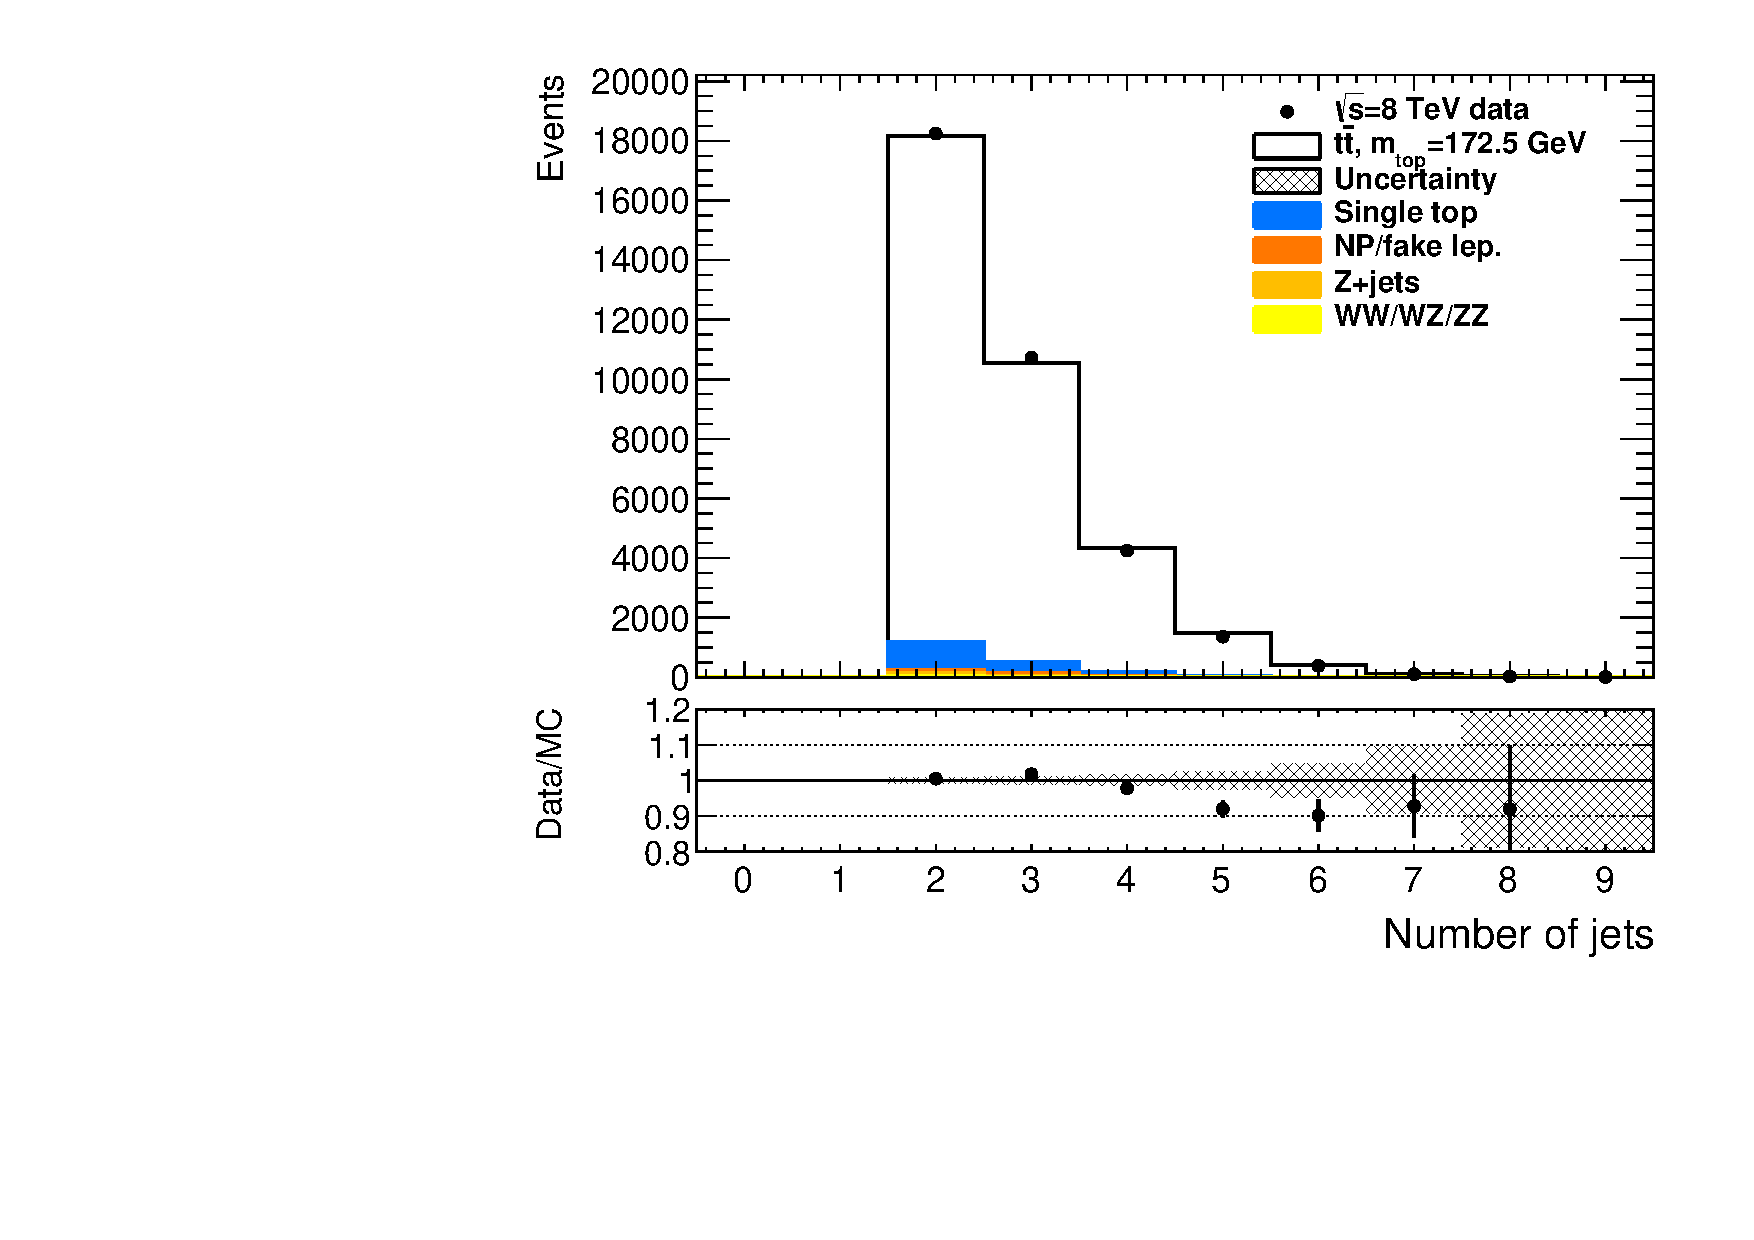
\includegraphics[width=0.49\textwidth]{./figs/fig_8TeV_TRC28_wp70/Dilep_SgnBkg_ratio_norm_sel3_n_jets.pdf}
  \label{sfig:n_jets_8TeV_standard}
}
\subfloat[Standard]{
% \subfloat[Number of \btagged\ jets]{
  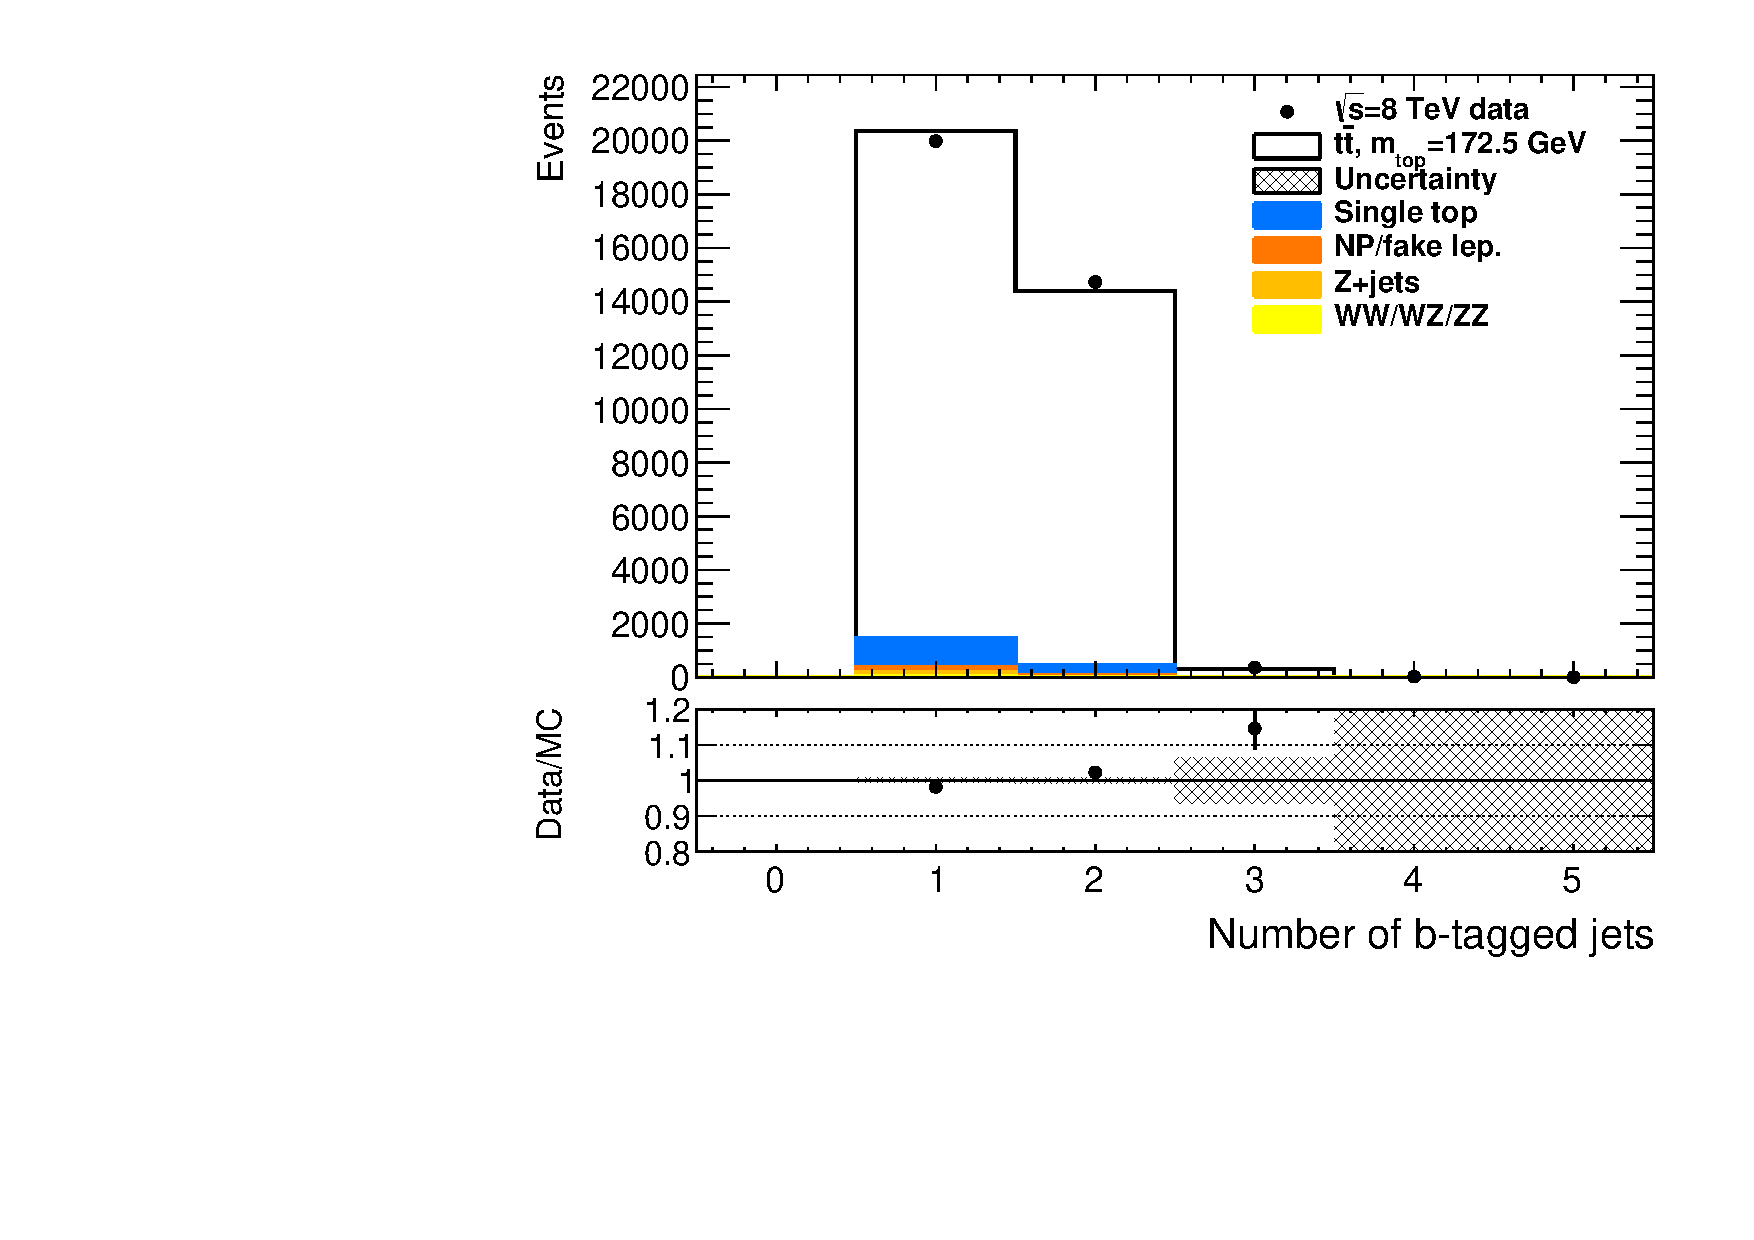
\includegraphics[width=0.49\textwidth]{./figs/fig_8TeV_TRC28_wp70/Dilep_SgnBkg_ratio_norm_sel3_n_bjets.pdf}
  \label{sfig:n_bjets_8TeV_standard}
}
\hfill
\subfloat[\Cutbased]{
% \subfloat[Number of jets]{
  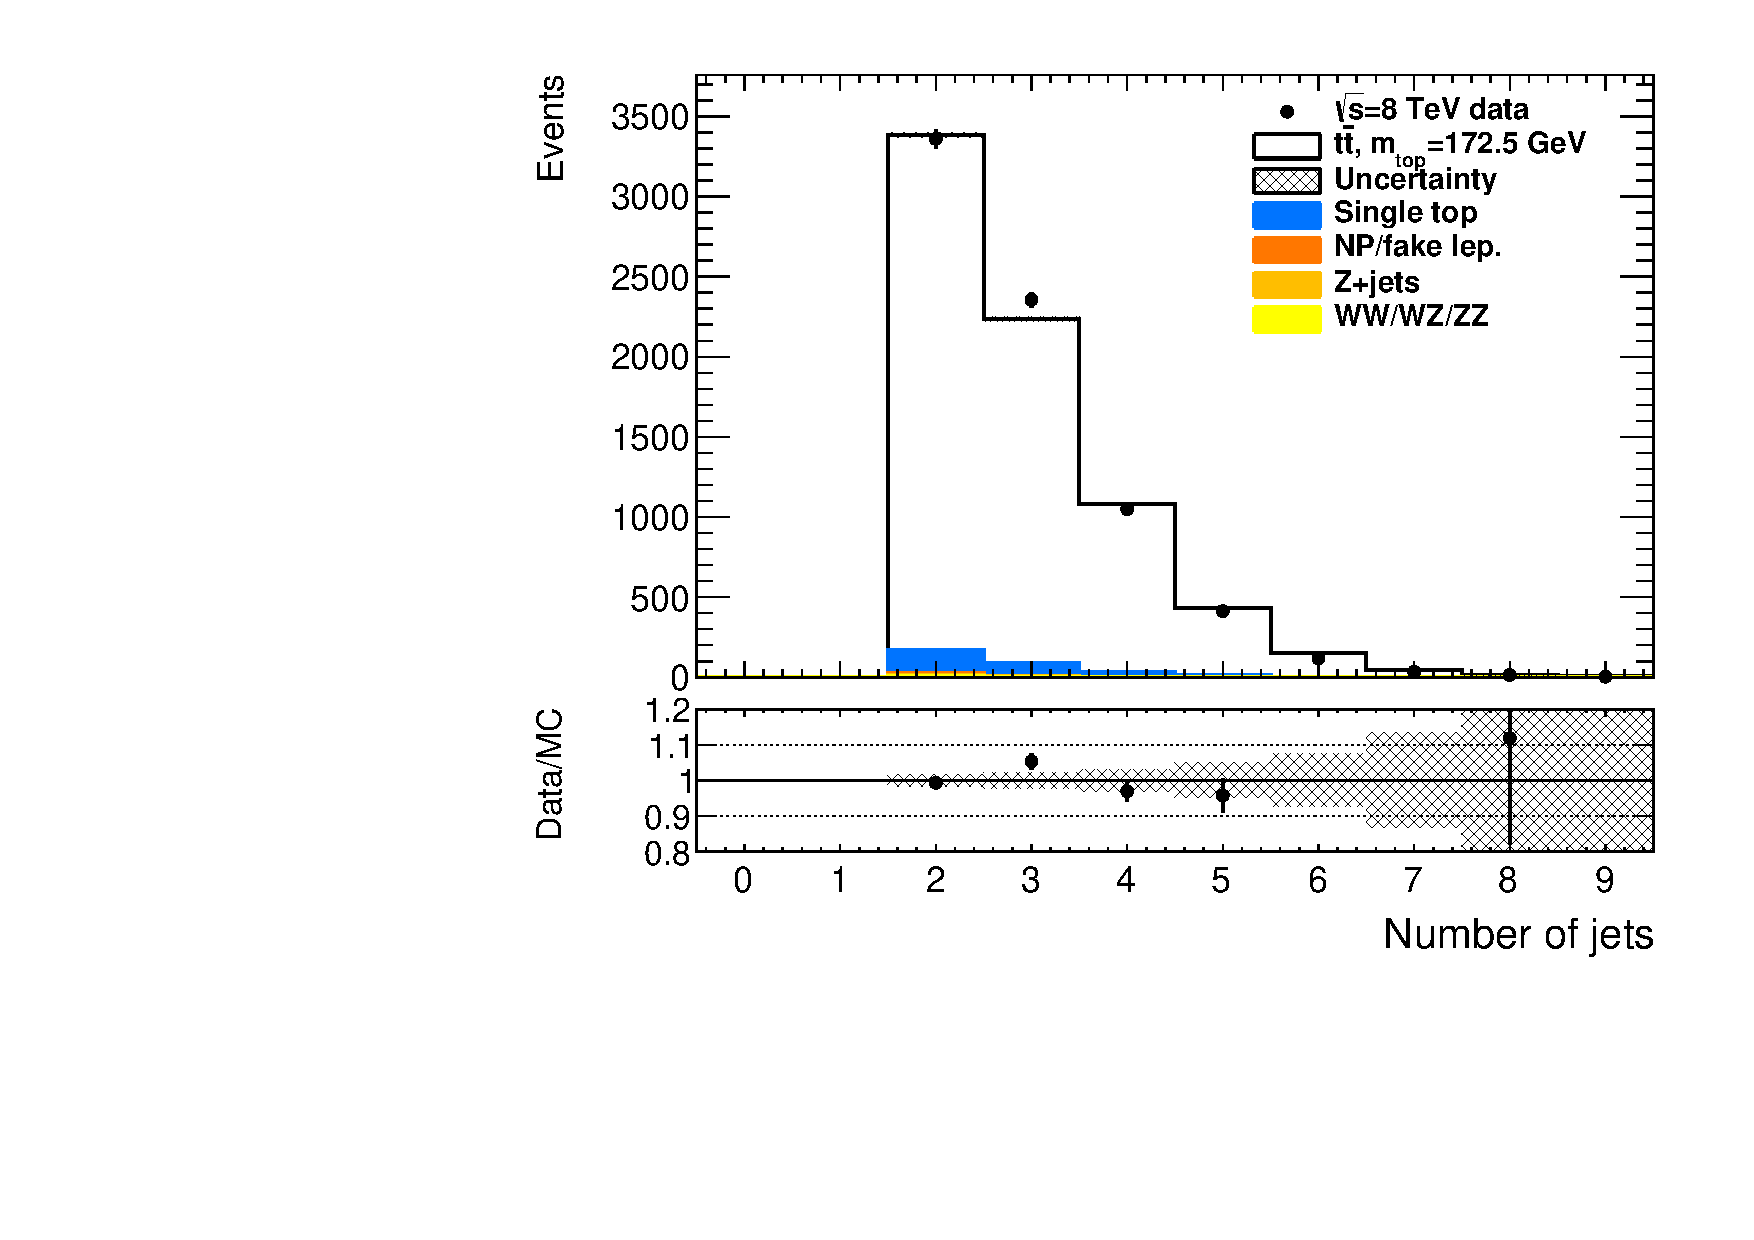
\includegraphics[width=0.49\textwidth]{./figs/fig_8TeV_TRC28_wp70_ptlb130/Dilep_SgnBkg_ratio_norm_sel3_n_jets.pdf}
  \label{sfig:n_jets_8TeV_cutbased}
}
\subfloat[\Cutbased]{
% \subfloat[Number of \btagged\ jets]{
  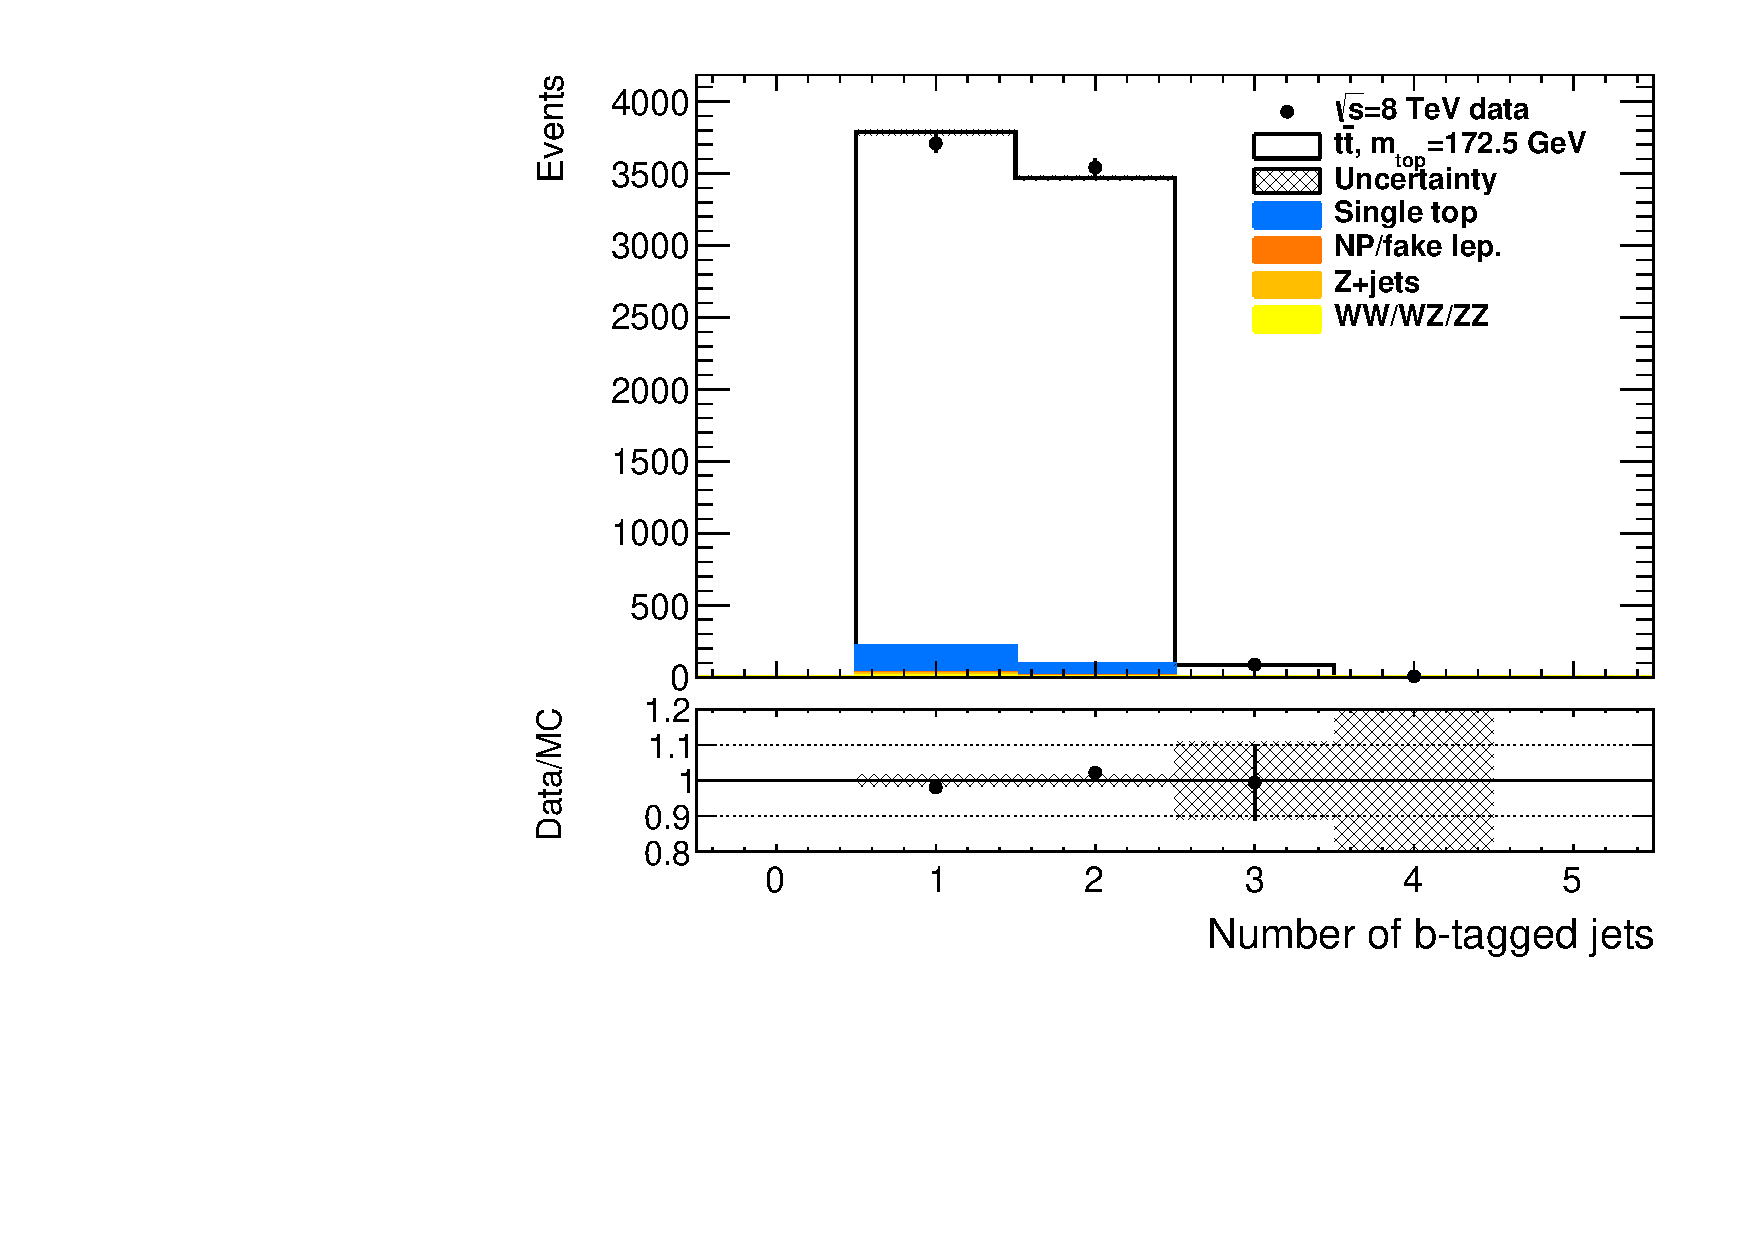
\includegraphics[width=0.49\textwidth]{./figs/fig_8TeV_TRC28_wp70_ptlb130/Dilep_SgnBkg_ratio_norm_sel3_n_bjets.pdf}
  \label{sfig:n_bjets_8TeV_cutbased}
}
\hfill
\subfloat[\Mvabased]{
% \subfloat[Number of jets]{
  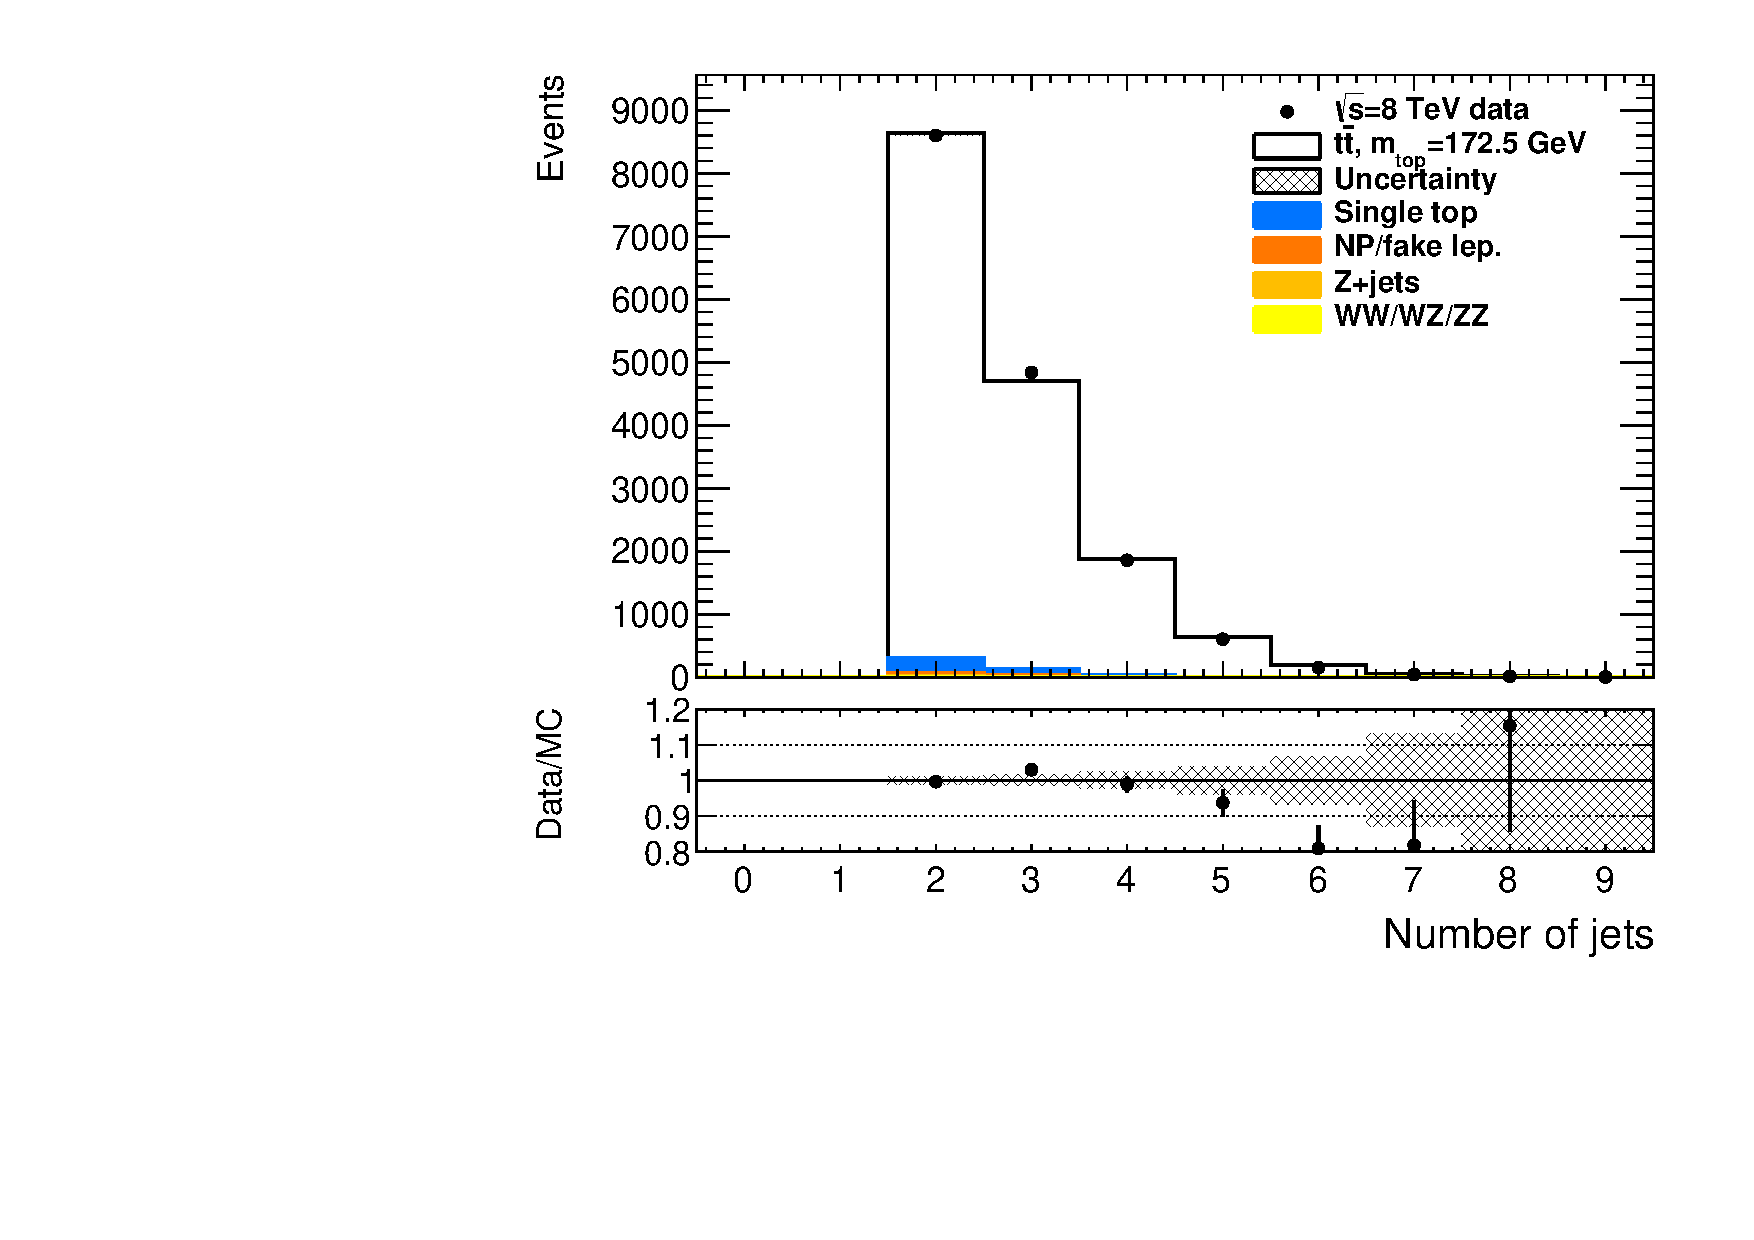
\includegraphics[width=0.49\textwidth]{./figs/fig_8TeV_TRC28_wp70_BDT-0.03/Dilep_SgnBkg_ratio_norm_sel3_n_jets.pdf}
  \label{sfig:n_jets_8TeV_mvabased}
}
\subfloat[\Mvabased]{
% \subfloat[Number of \btagged\ jets]{
  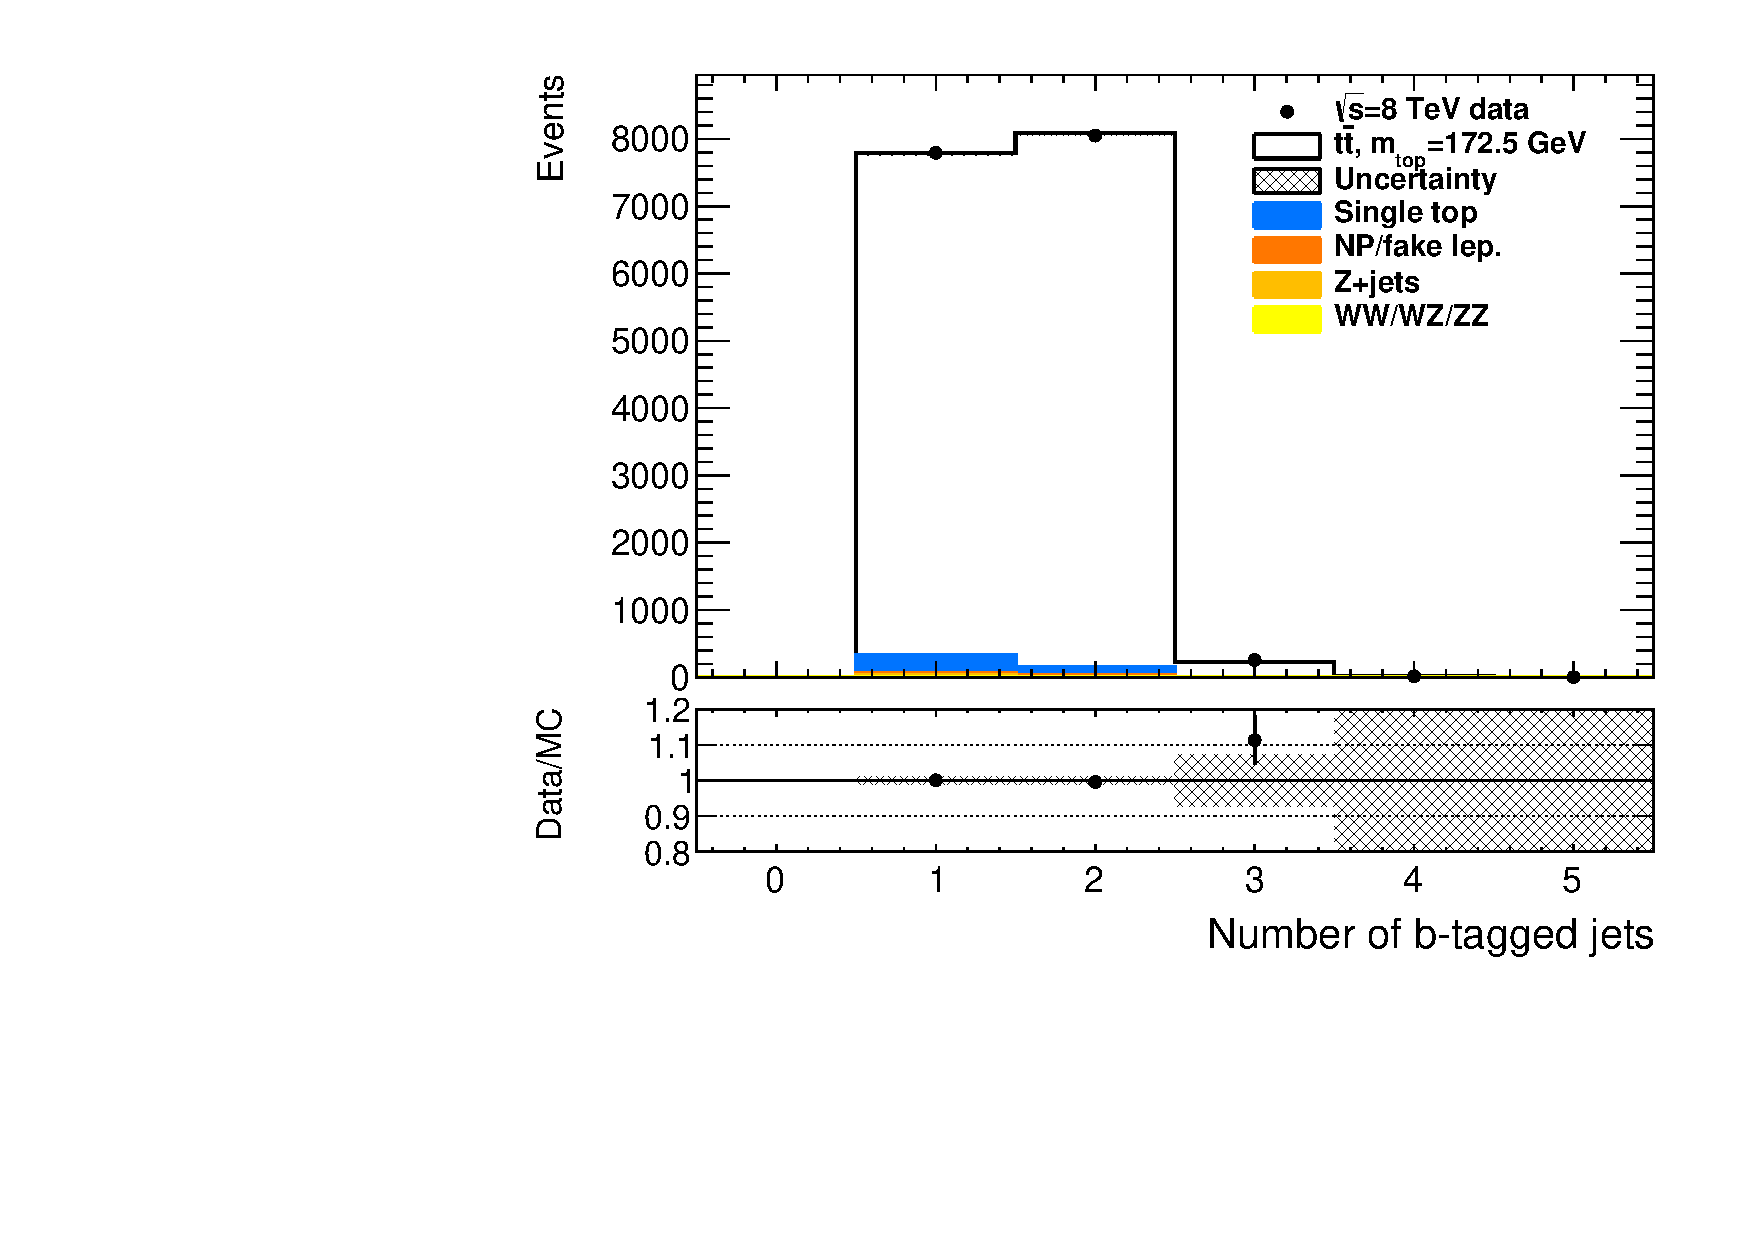
\includegraphics[width=0.49\textwidth]{./figs/fig_8TeV_TRC28_wp70_BDT-0.03/Dilep_SgnBkg_ratio_norm_sel3_n_bjets.pdf}
  \label{sfig:n_bjets_8TeV_mvabased}
}
%
% \caption[Data to \gls{MC} comparison for $\sqrts=8$~\TeV\ data]{
\caption[Data to \gls{MC} comparison for $\sqrts=8$~\TeV\ data: jet multiplicities]{
%
Kinematic distributions normalised to the data observation after the standard, the \cutbased\ and the \mvabased\ event selection with at least one \btagged\ jet. 
%
The figures show the measured jet and \btagged\ jet multiplicities on the left and on the right, respectively.
%
The prediction (solid histogram) is normalised to the data (points).
%
The hatched area is the combined uncertainty on the prediction, described in \sect~\ref{sect:dataMC8TeV}, and the rightmost bin contains the overflow, if present. The uncertainty bars of the data correspond to the statistical uncertainty.
%
For each figure, the ratio of the data to the \gls{MC} prediction is also presented.
%
\label{fig:DL_dataMC_njets}}
\end{figure*}
%%%%%%%%%%%%%%%%%%%%%%%%%%%%%%%%%%%%%%%%%%%%%%%%%%%%%%%%%%%%%%%%%%%%%%%%%%%%%
% 
%%%%%%%%%%%%%%%%%%%%%%%%%%%%%%%%%%%%%%%%%%%%%%%%%%%%%%%%%%%%%%%%%%%%%%%%%%%%%%%
\begin{figure*}[tbp!]
\centering
\subfloat[Standard]{
% \subfloat[\btagged\ jet \pt]{
  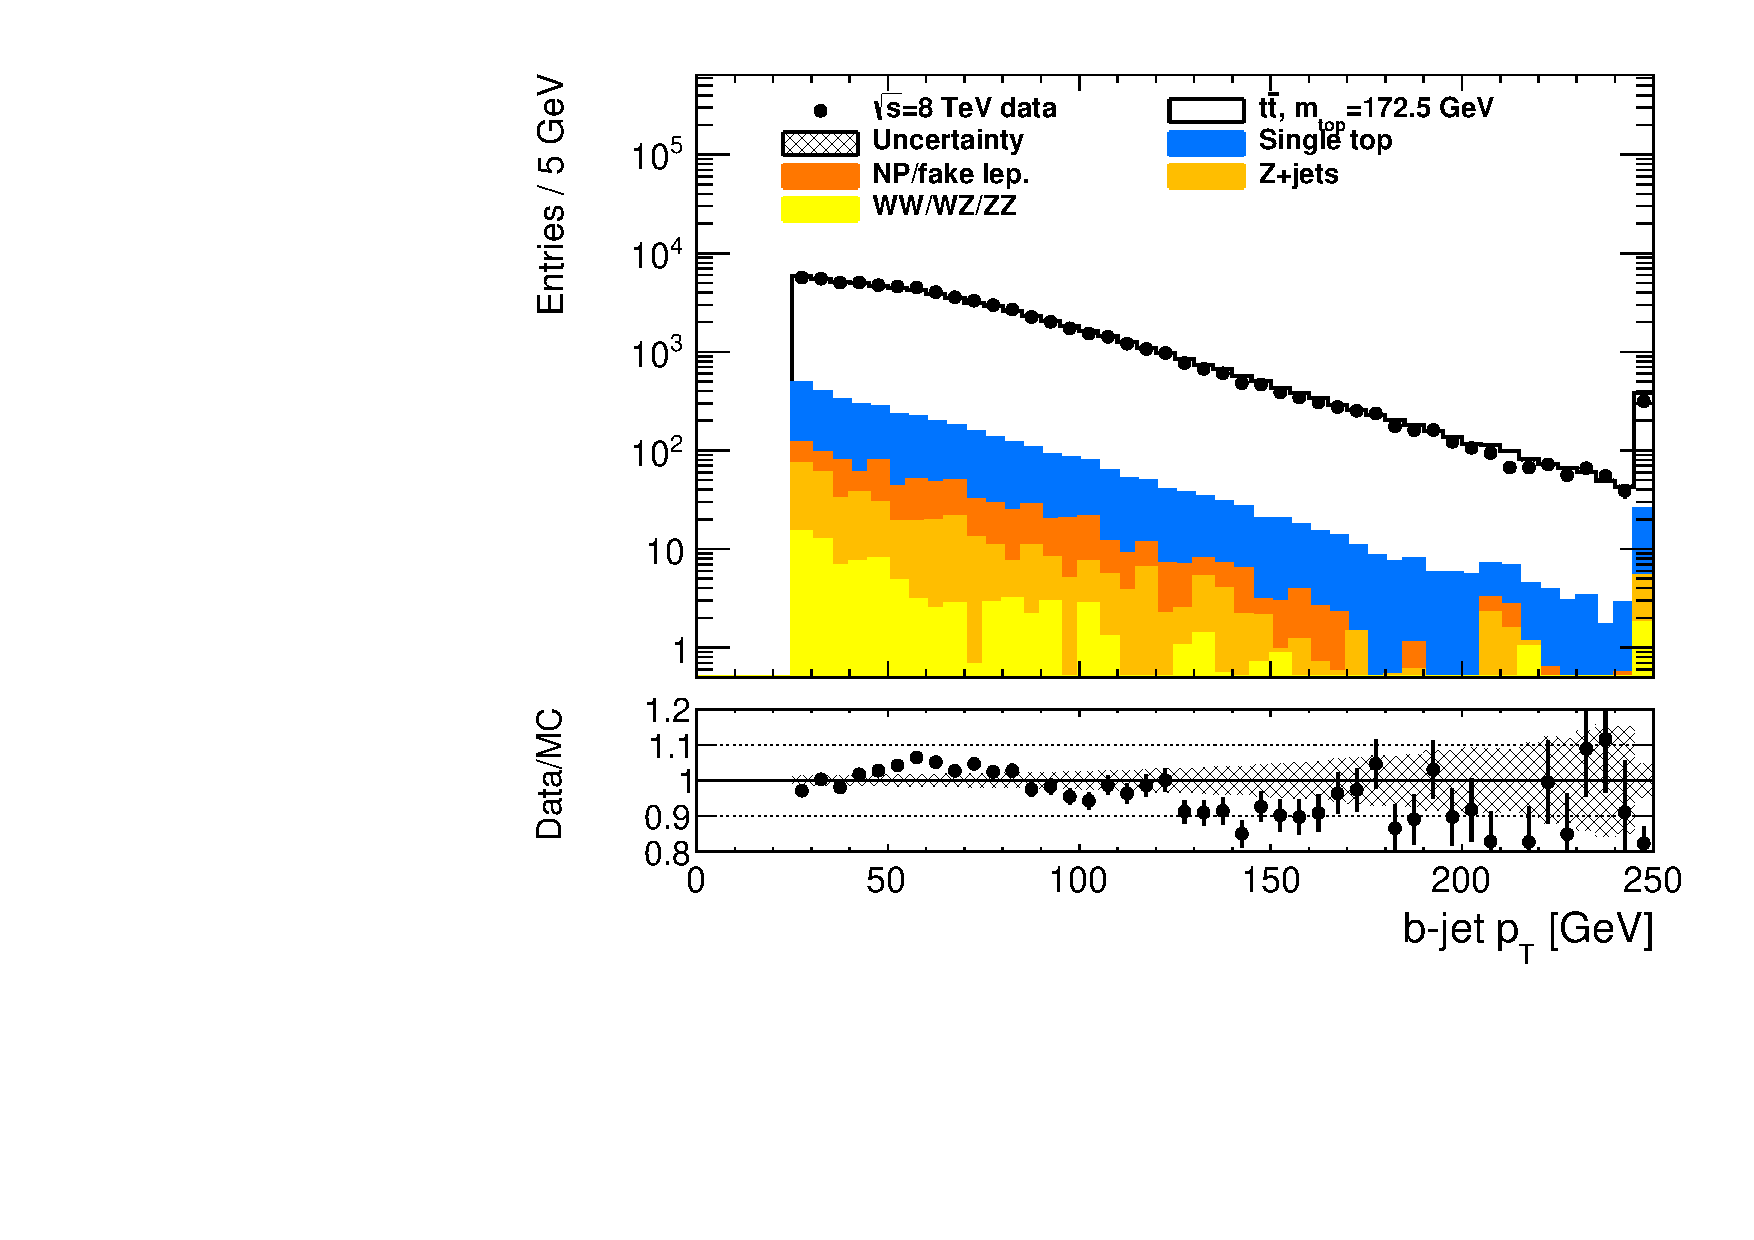
\includegraphics[width=0.49\textwidth]{./figs/fig_8TeV_TRC28_wp70/Dilep_SgnBkg_ratio_norm_sel3_bJet_Pt_logscale.pdf}
  \label{sfig:bJet_Pt_8TeV_standard}
}
\subfloat[Standard]{
% \subfloat[Lepton \pt]{
  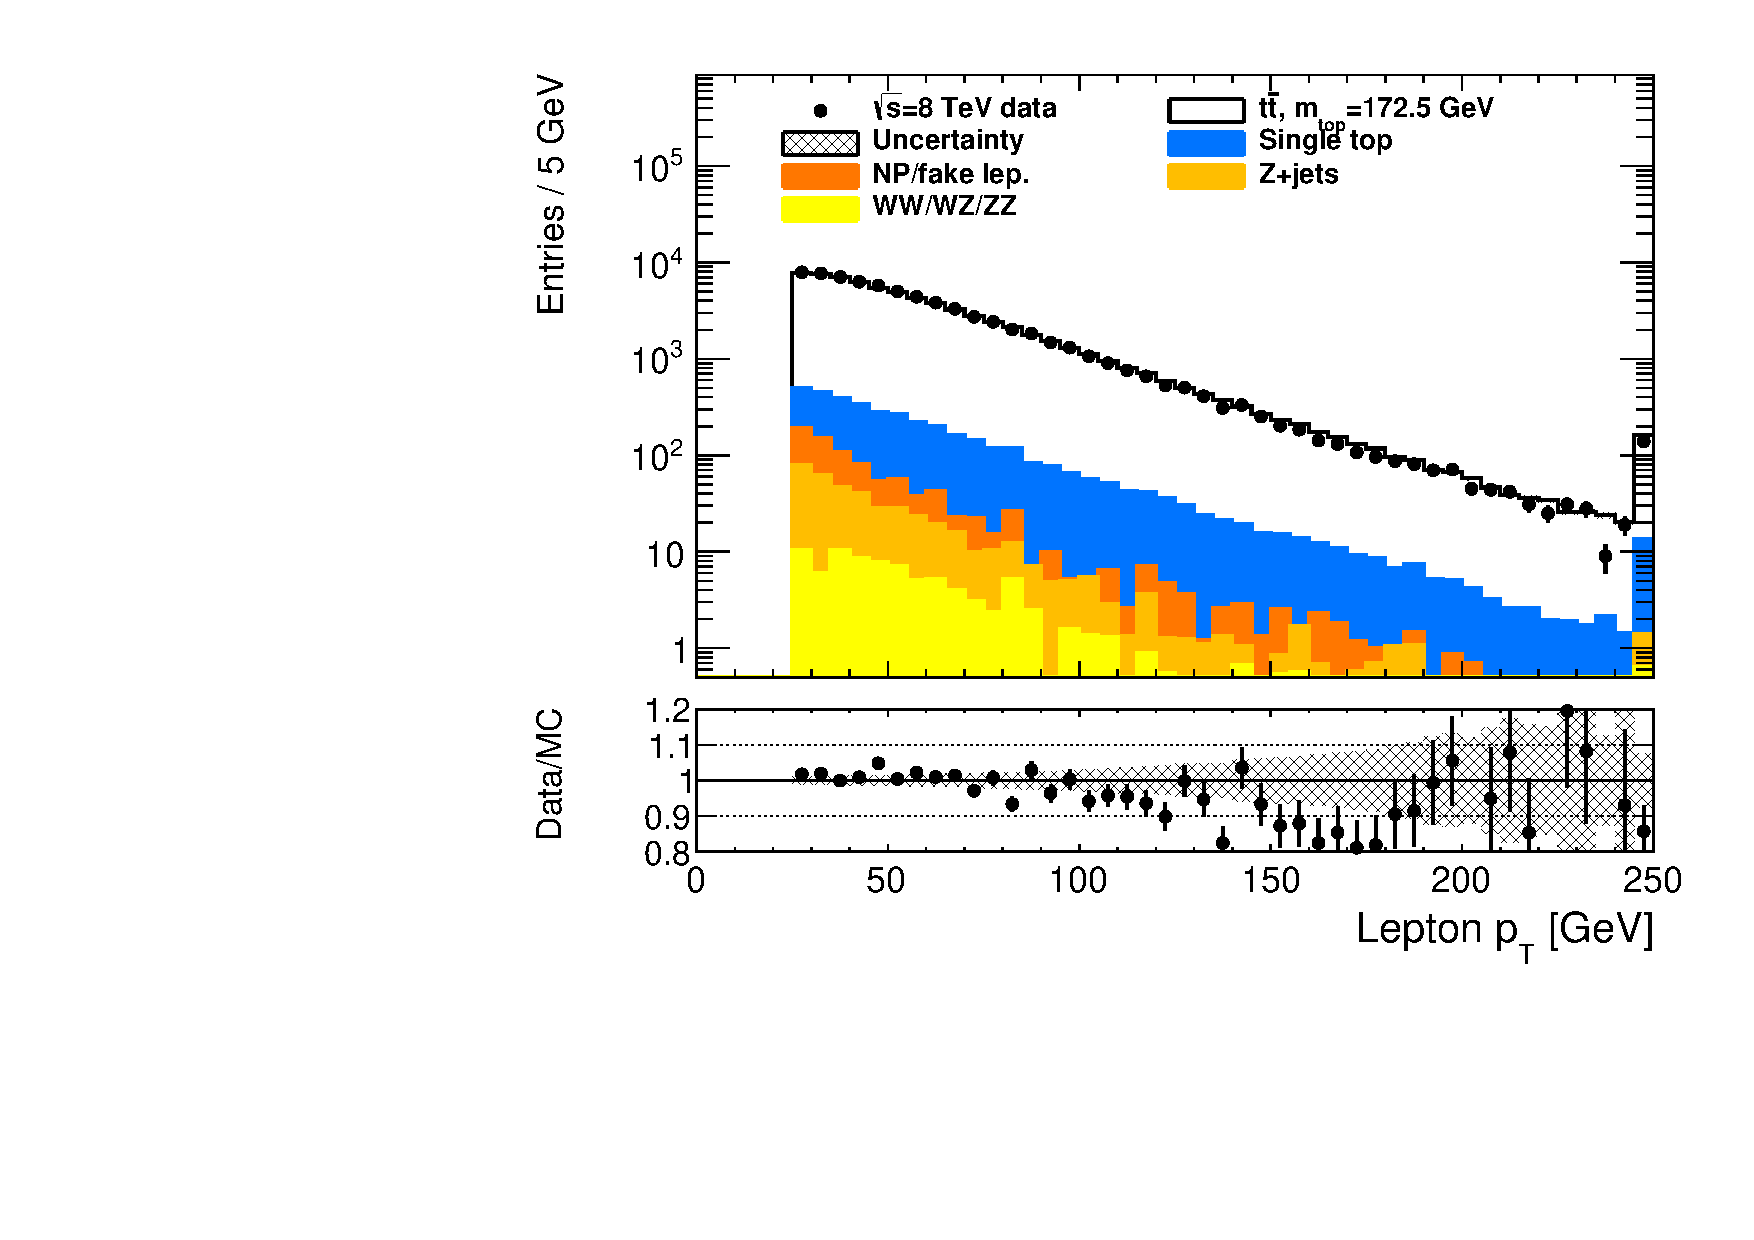
\includegraphics[width=0.49\textwidth]{./figs/fig_8TeV_TRC28_wp70/Dilep_SgnBkg_ratio_norm_sel3_Lep_Pt_logscale.pdf}
  \label{sfig:Lep_Pt_8TeV_standard}
}
\hfill
\subfloat[\Cutbased]{
% \subfloat[\btagged\ jet \pt]{
  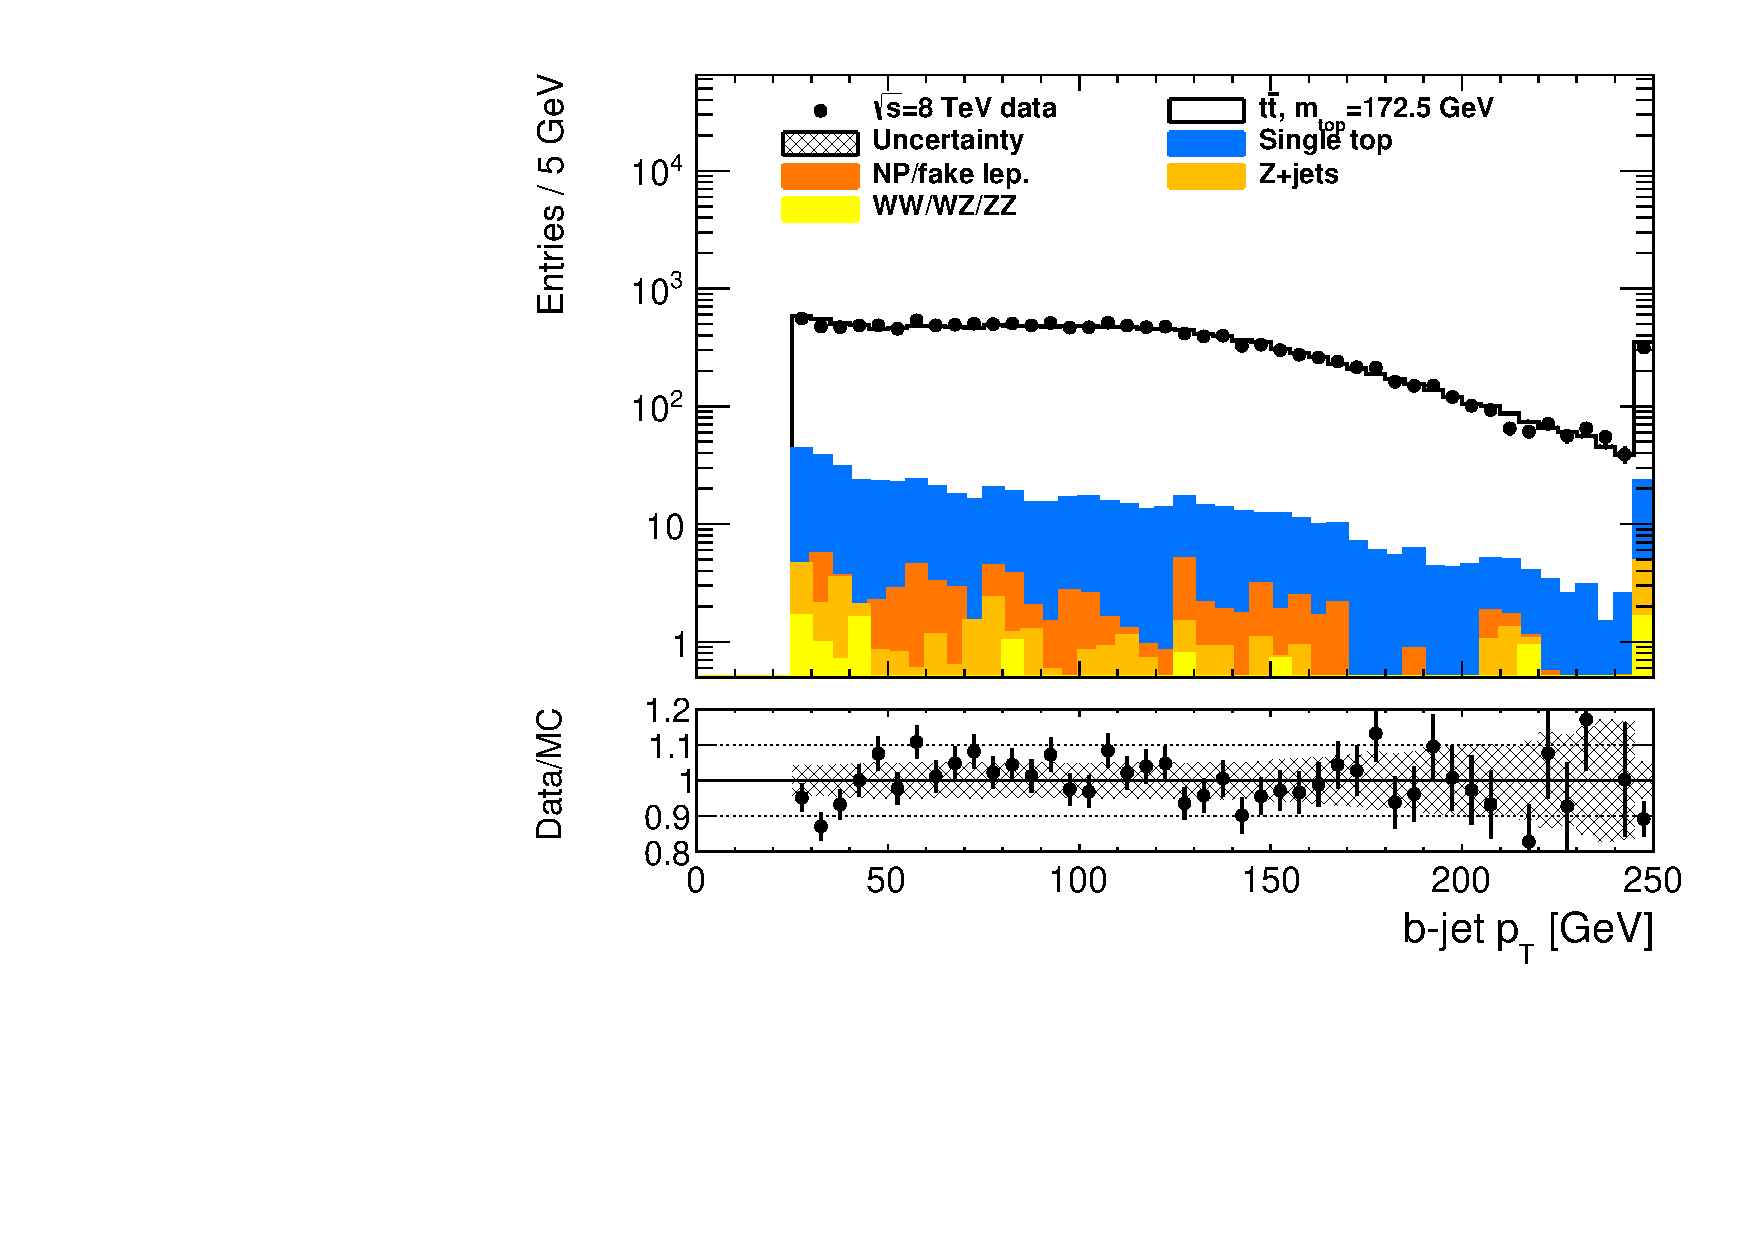
\includegraphics[width=0.49\textwidth]{./figs/fig_8TeV_TRC28_wp70_ptlb130/Dilep_SgnBkg_ratio_norm_sel3_bJet_Pt_logscale.pdf}
  \label{sfig:bJet_Pt_8TeV_cutbased}
}
\subfloat[\Cutbased]{
% \subfloat[Lepton \pt]{
  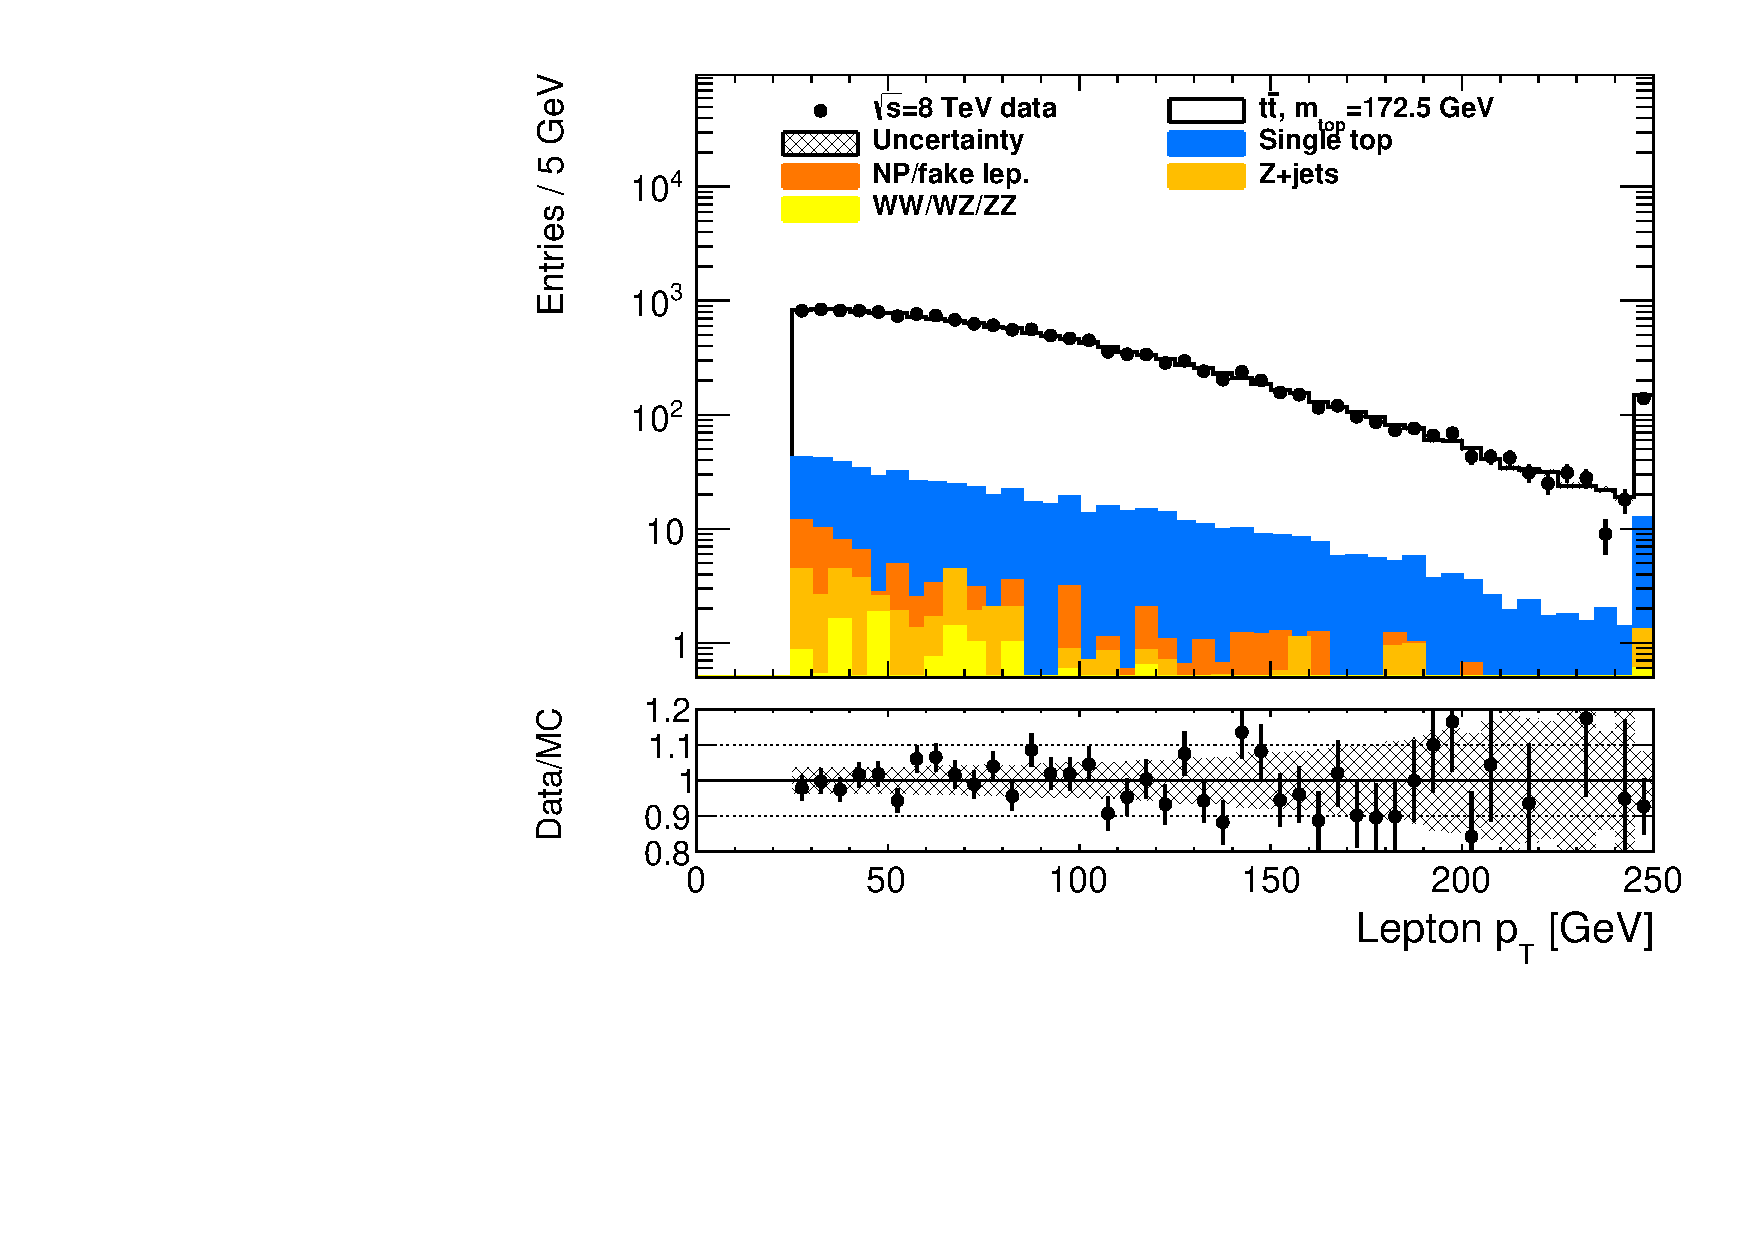
\includegraphics[width=0.49\textwidth]{./figs/fig_8TeV_TRC28_wp70_ptlb130/Dilep_SgnBkg_ratio_norm_sel3_Lep_Pt_logscale.pdf}
  \label{sfig:Lep_Pt_8TeV_cutbased}
}
\hfill
\subfloat[\Mvabased]{
% \subfloat[\btagged\ jet \pt]{
  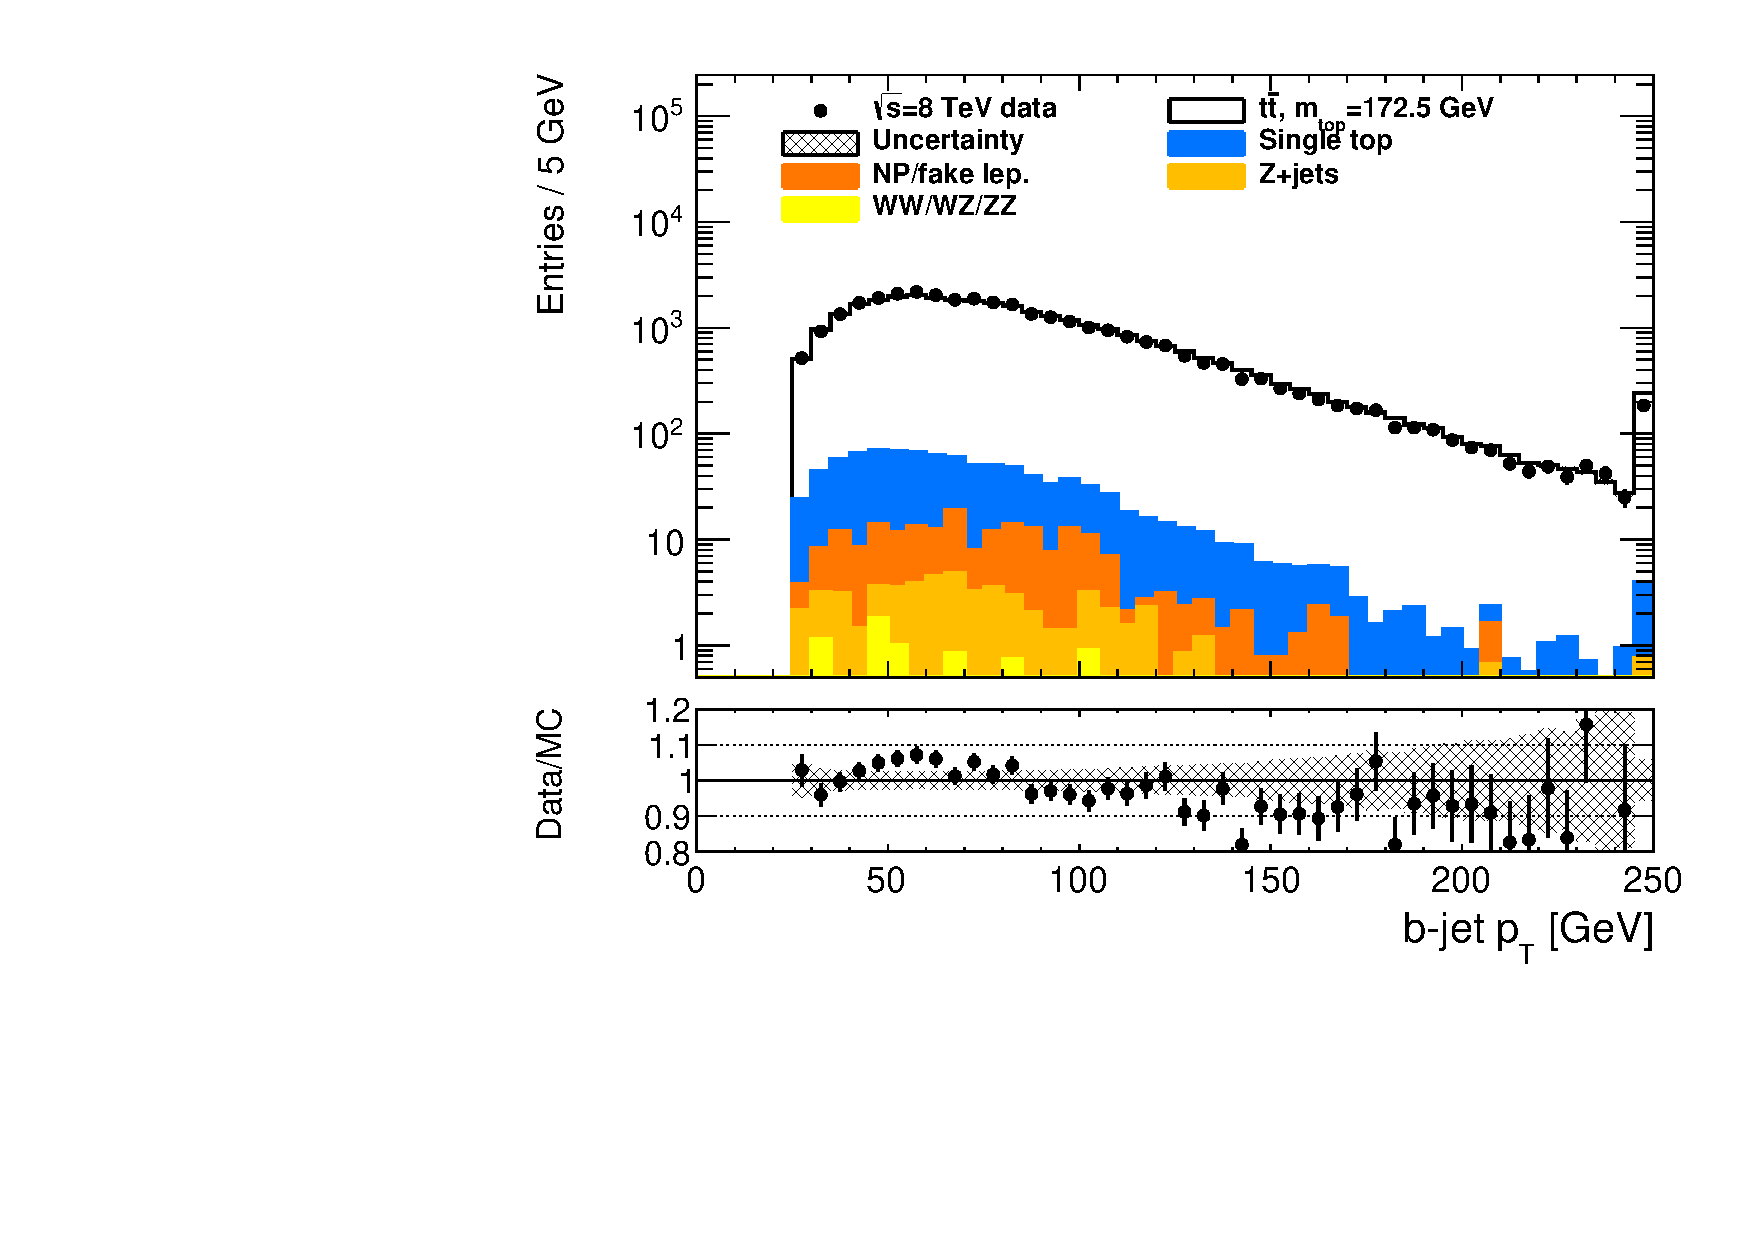
\includegraphics[width=0.49\textwidth]{./figs/fig_8TeV_TRC28_wp70_BDT-0.03/Dilep_SgnBkg_ratio_norm_sel3_bJet_Pt_logscale.pdf}
  \label{sfig:bJet_Pt_8TeV_mvabased}
}
\subfloat[\Mvabased]{
% \subfloat[Lepton \pt]{
  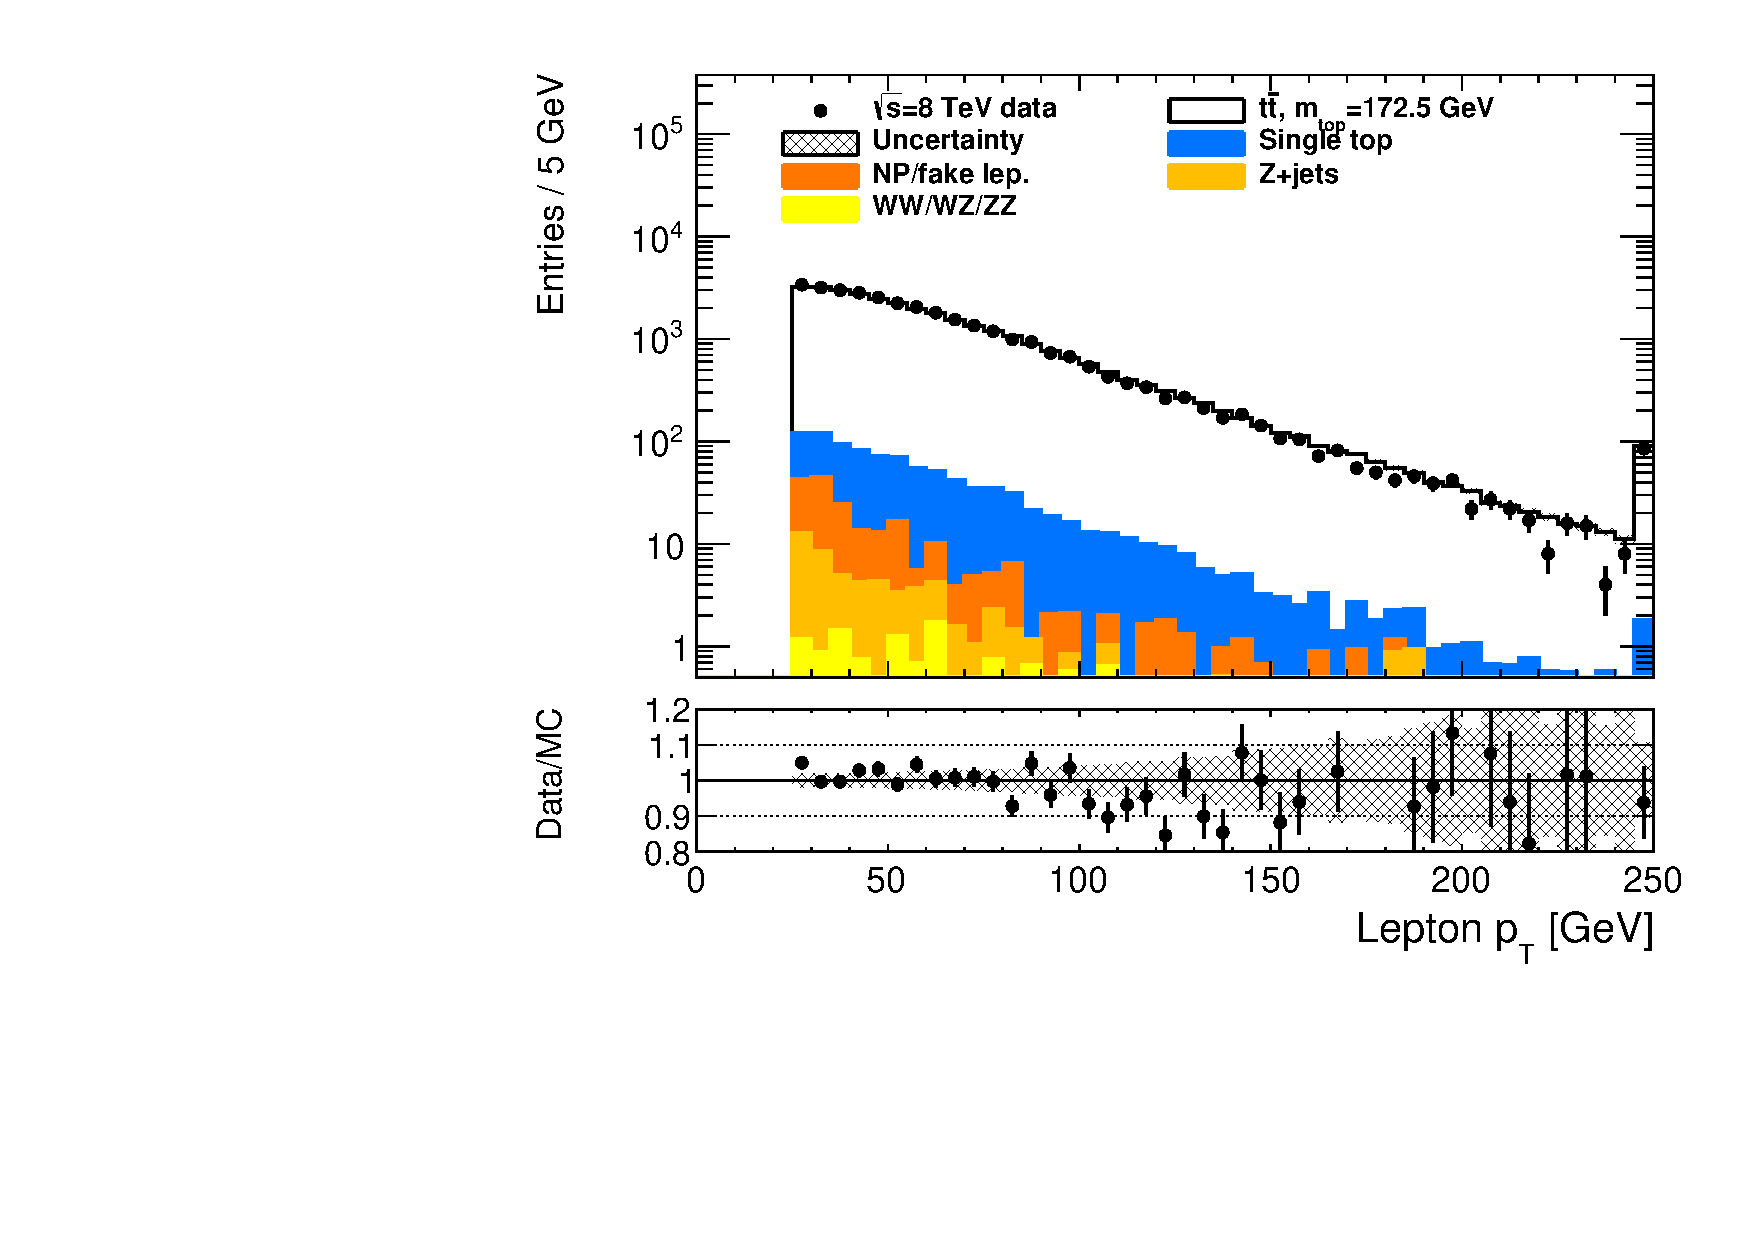
\includegraphics[width=0.49\textwidth]{./figs/fig_8TeV_TRC28_wp70_BDT-0.03/Dilep_SgnBkg_ratio_norm_sel3_Lep_Pt_logscale.pdf}
  \label{sfig:Lep_Pt_8TeV_mvabased}
}
%
% \caption[Data to \gls{MC} comparison for $\sqrts=8$~\TeV\ data]{
\caption[Data to \gls{MC} comparison for $\sqrts=8$~\TeV\ data: \pt]{
%
Same as \fig~\ref{fig:DL_dataMC_njets} but showing the \bjet\ \pt\ on the left and the lepton \pt\ distributions on the right.
%
\label{fig:DL_dataMC_pt}}
\end{figure*}
%%%%%%%%%%%%%%%%%%%%%%%%%%%%%%%%%%%%%%%%%%%%%%%%%%%%%%%%%%%%%%%%%%%%%%%%%%%%%
% %
% %%%%%%%%%%%%%%%%%%%%%%%%%%%%%%%%%%%%%%%%%%%%%%%%%%%%%%%%%%%%%%%%%%%%%%%%%%%%%%%
\begin{figure*}[tbp!]
\centering
\subfloat[Standard]{
% \subfloat[\ptlb]{
  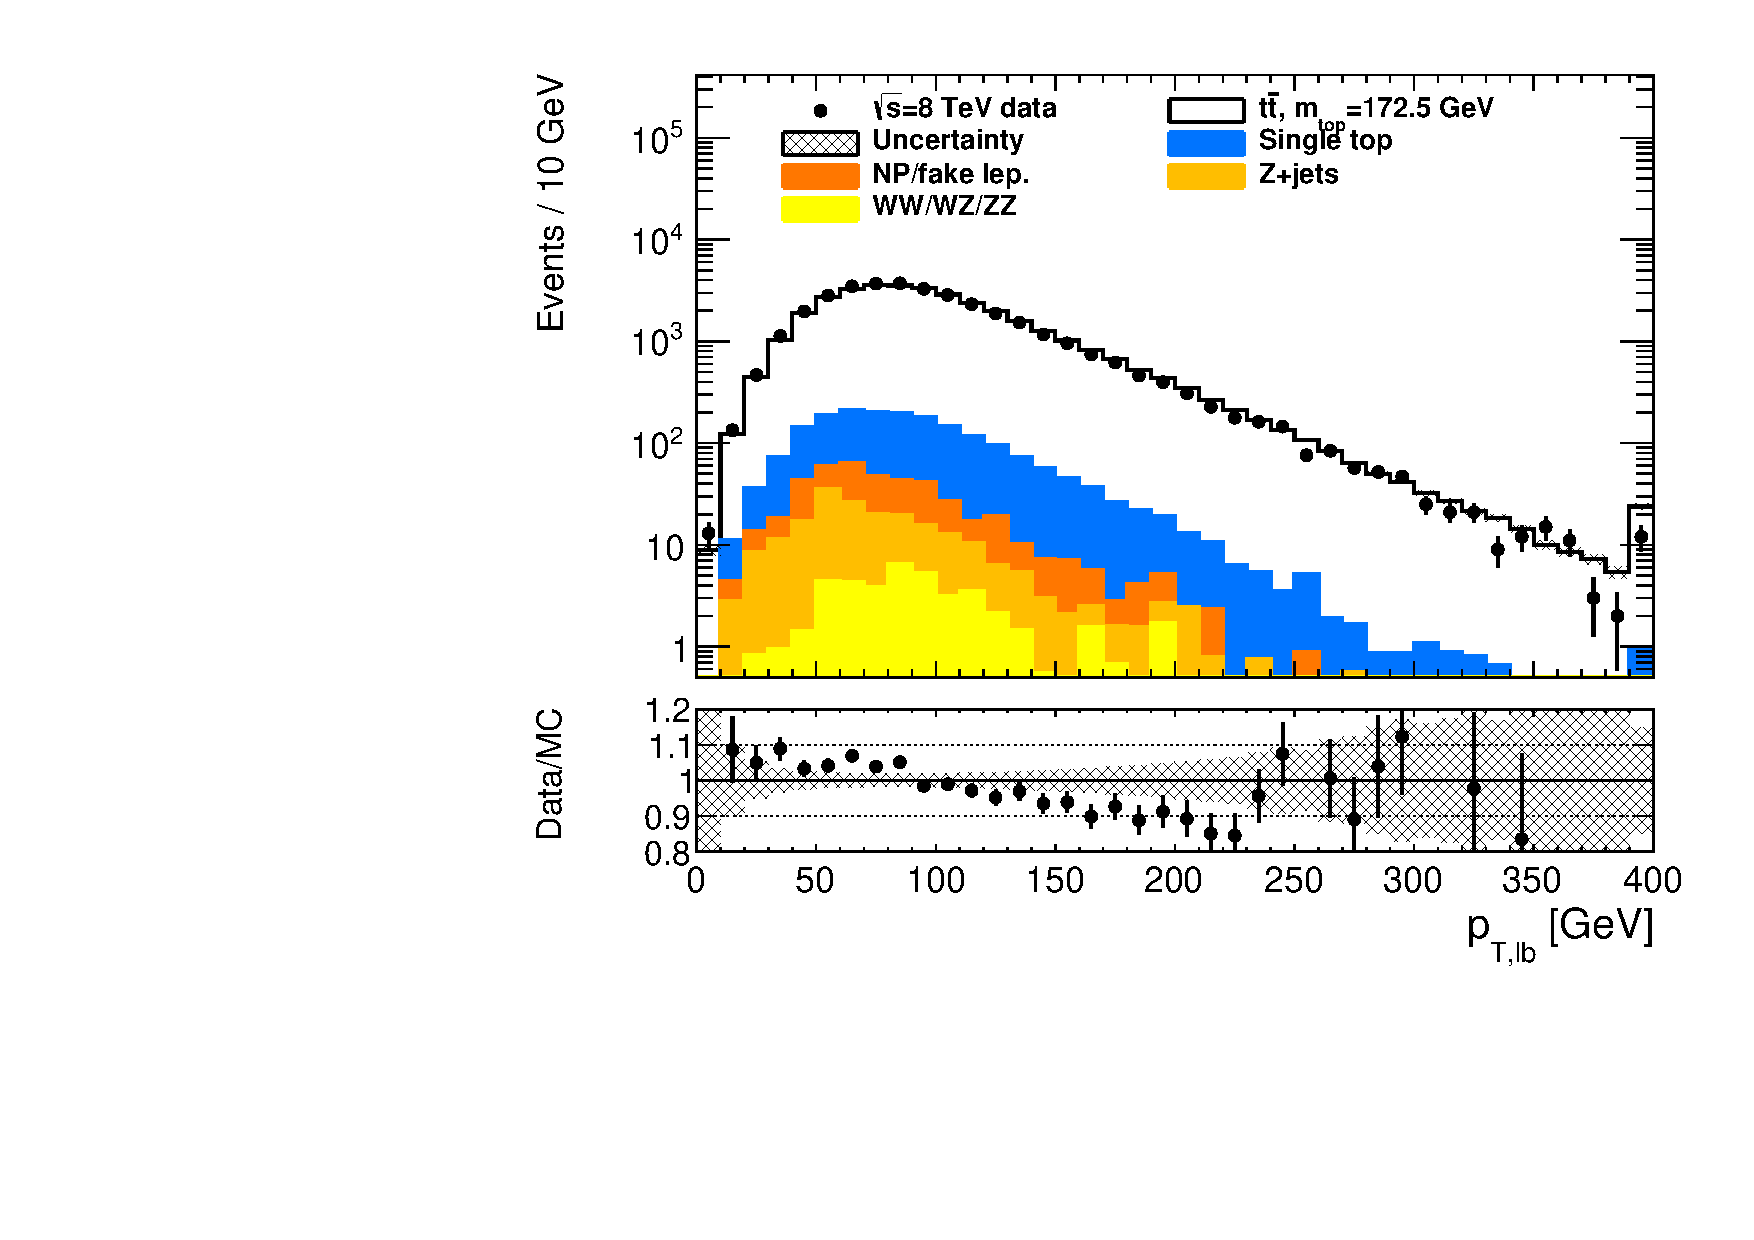
\includegraphics[width=0.49\textwidth]{./figs/fig_8TeV_TRC28_wp70/Dilep_SgnBkg_ratio_norm_sel3_ptlb_logscale.pdf}
  \label{sfig:ptlb_8TeV_standard}
}
\subfloat[Standard]{
% \subfloat[$\dR_{\ell b}$]{
  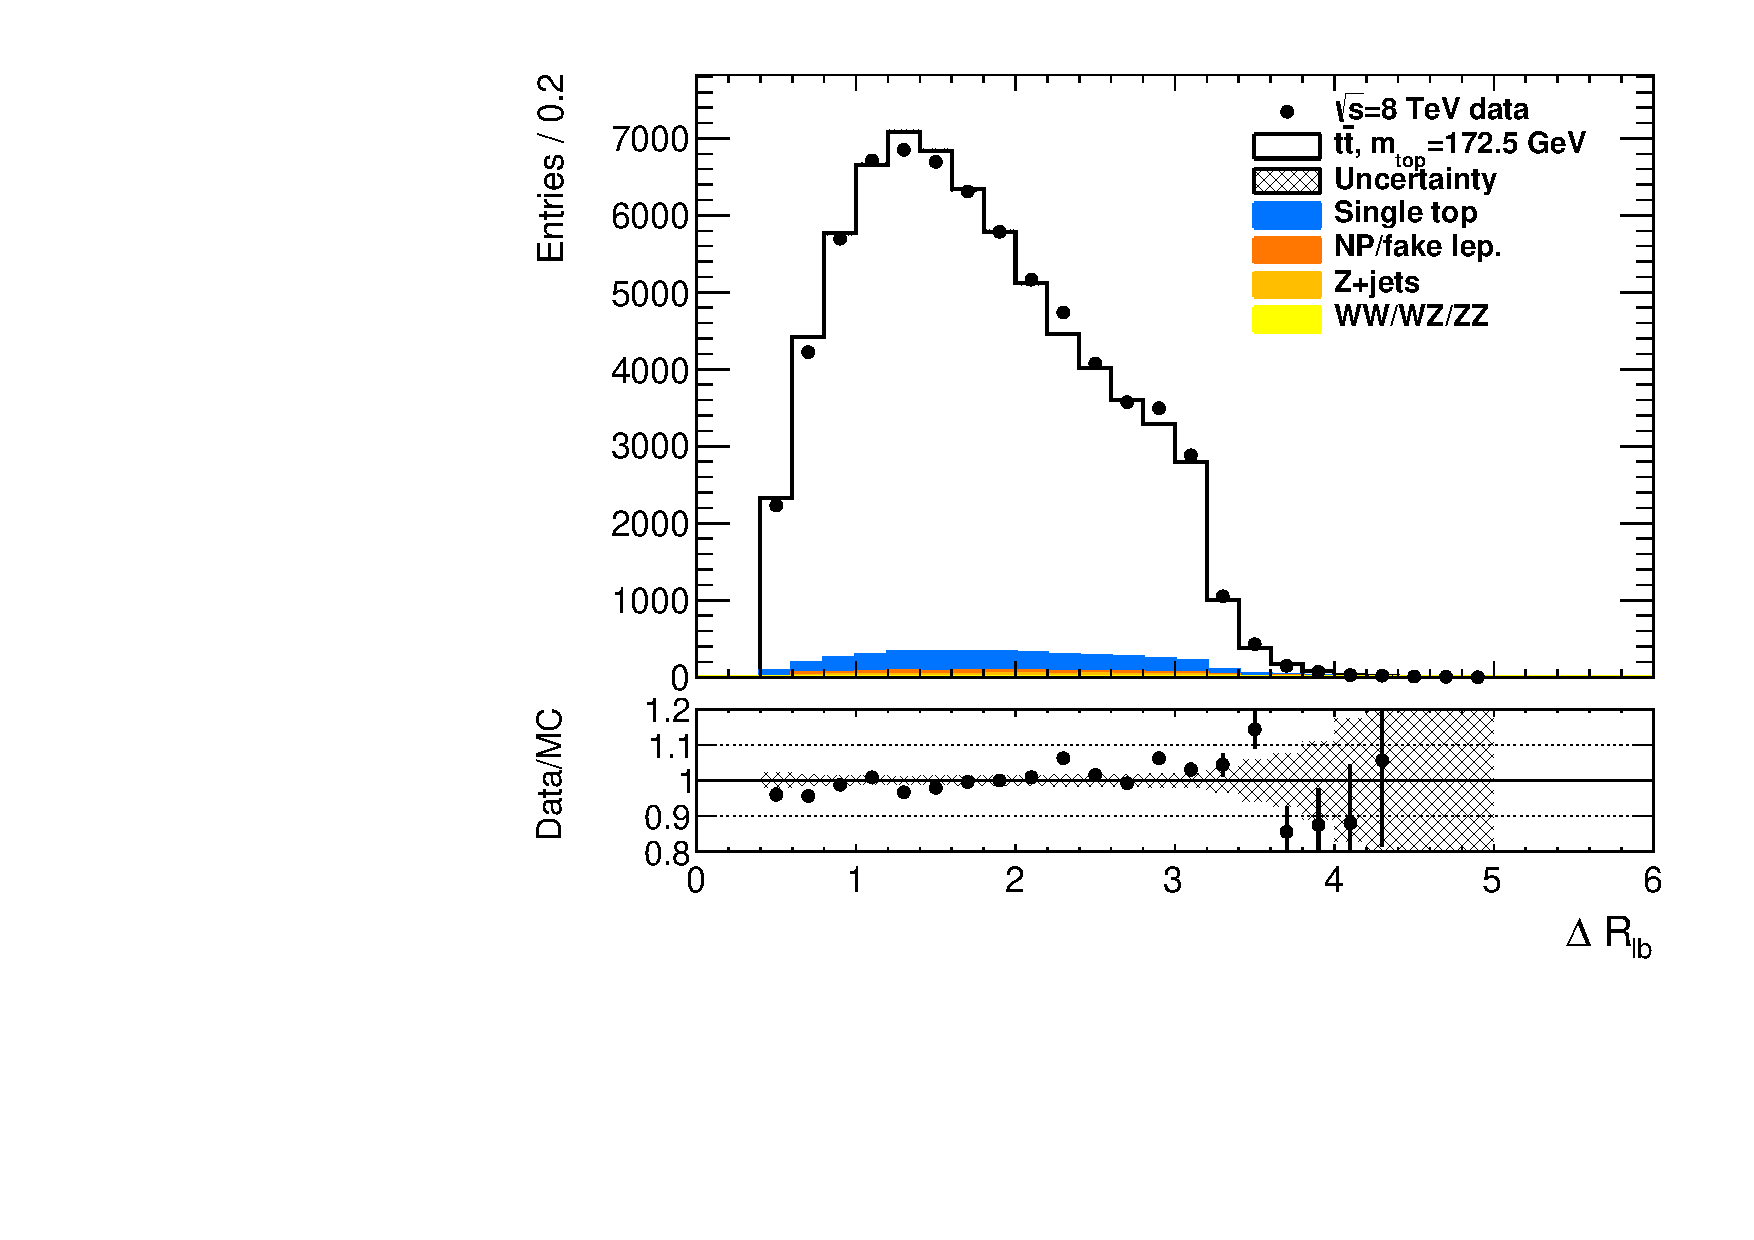
\includegraphics[width=0.49\textwidth]{./figs/fig_8TeV_TRC28_wp70/Dilep_SgnBkg_ratio_norm_sel3_dR_lb.pdf}
  \label{sfig:dR_lb_8TeV_standard}
}
\hfill
\subfloat[\Cutbased]{
% \subfloat[\ptlb]{
  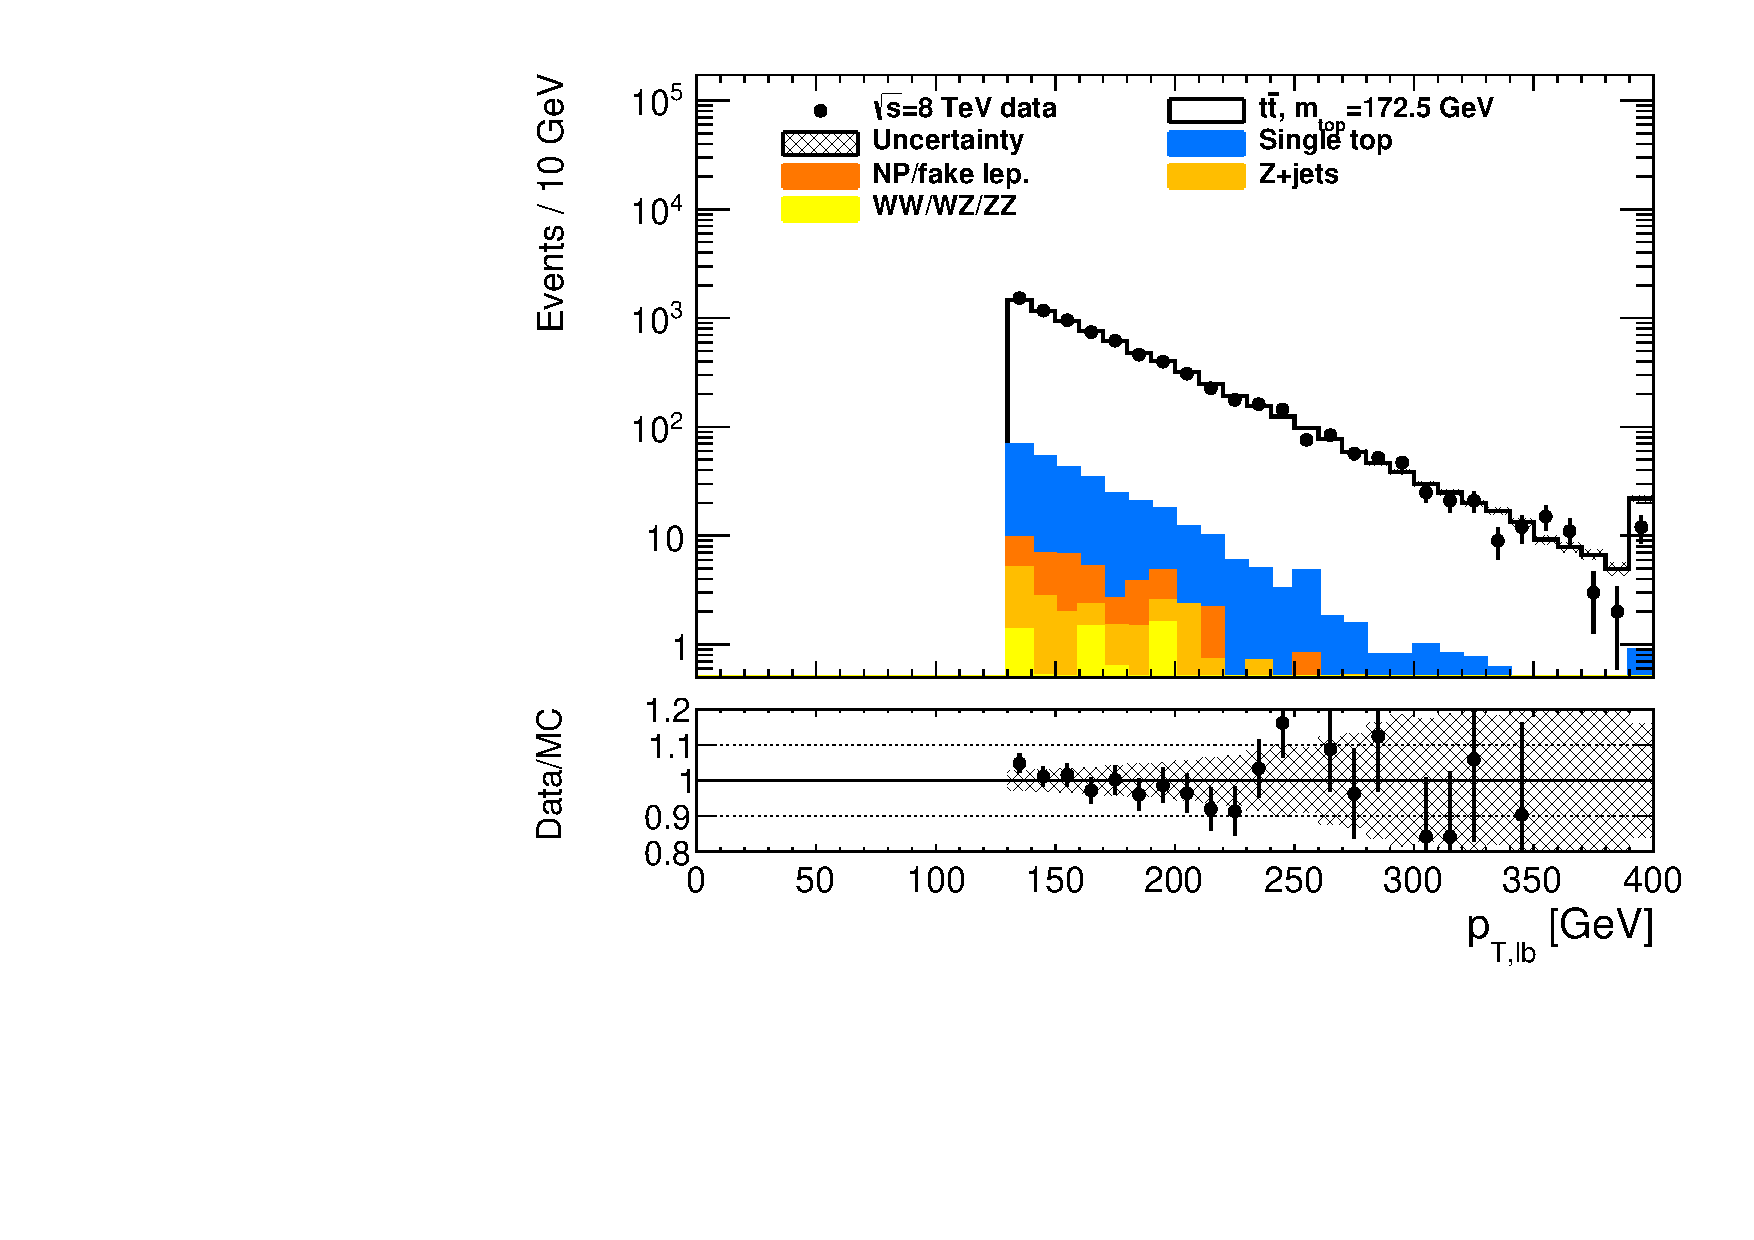
\includegraphics[width=0.49\textwidth]{./figs/fig_8TeV_TRC28_wp70_ptlb130/Dilep_SgnBkg_ratio_norm_sel3_ptlb_logscale.pdf}
  \label{sfig:ptlb_8TeV_cutbased}
}
\subfloat[\Cutbased]{
% \subfloat[$\dR_{\ell b}$]{
  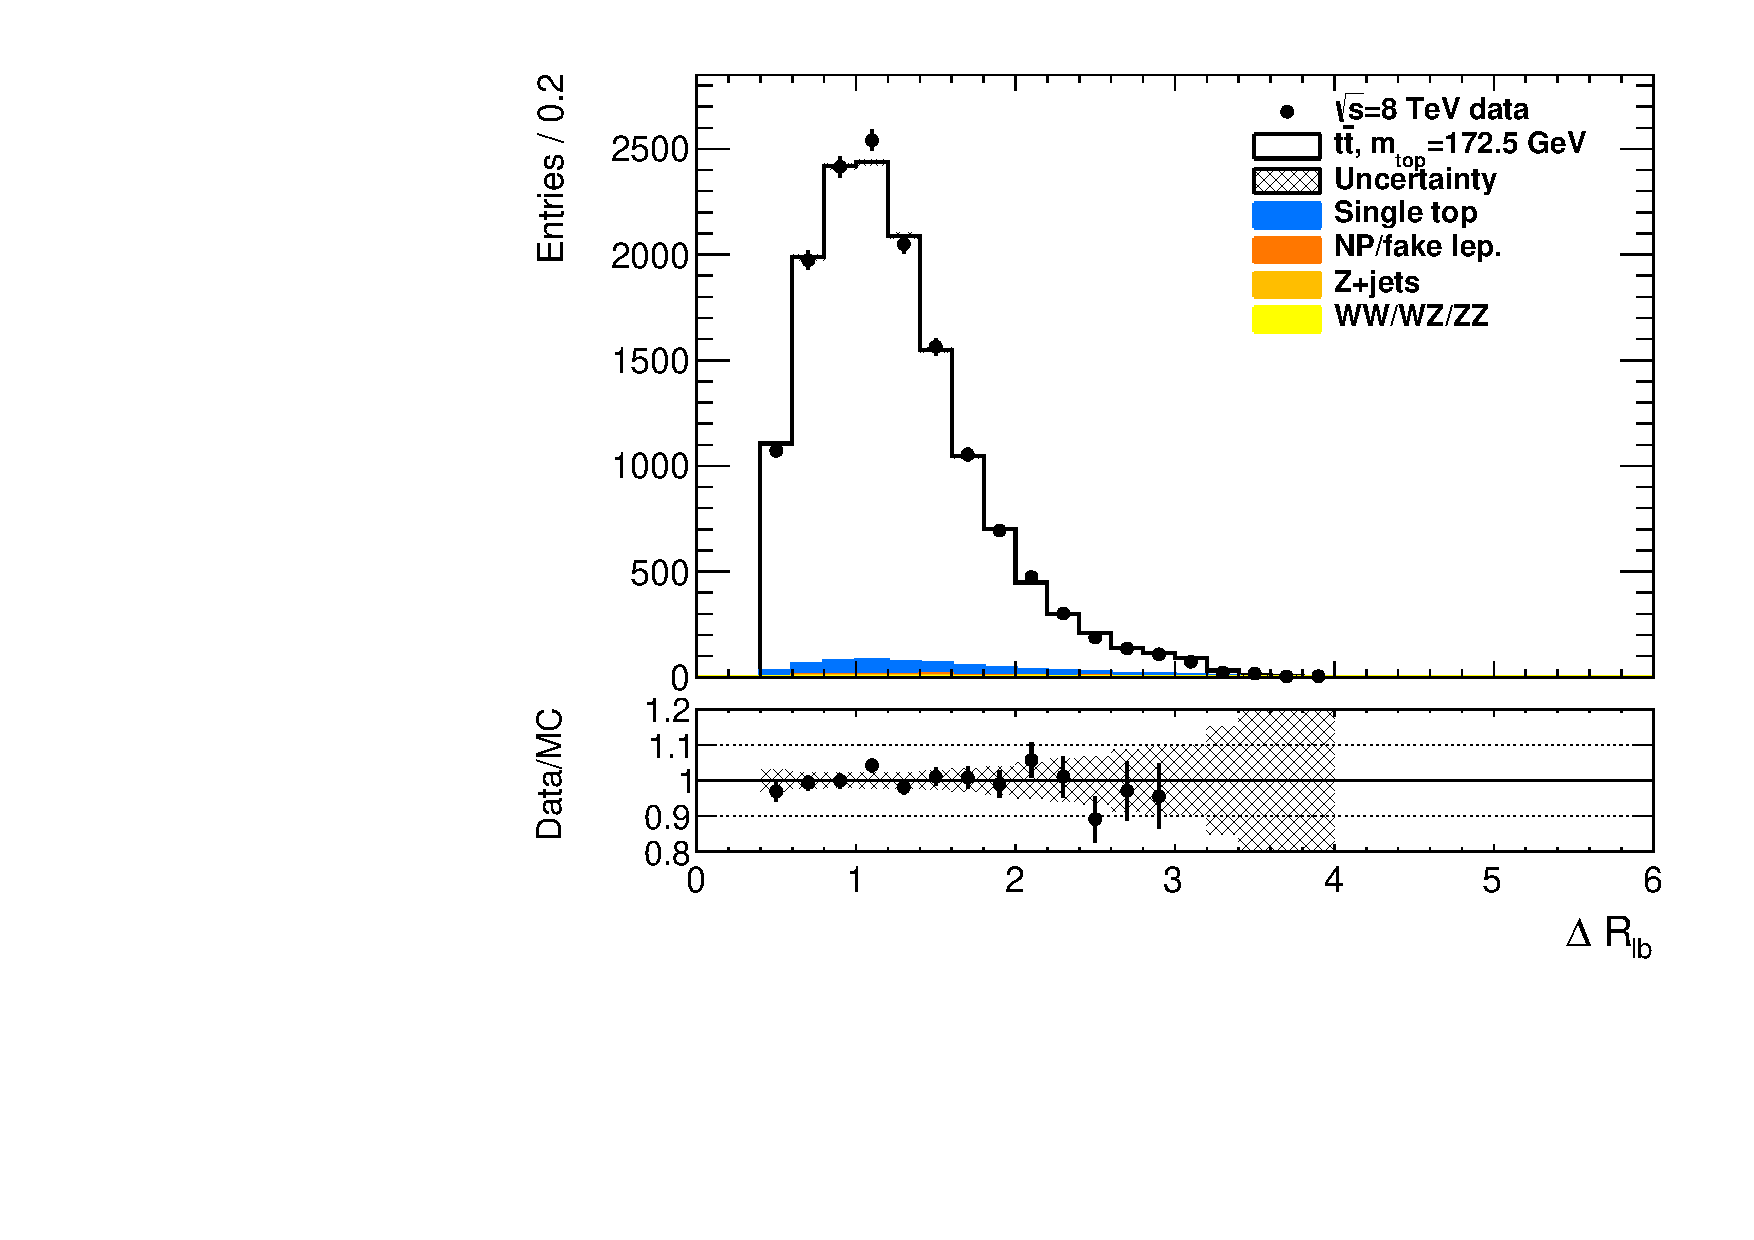
\includegraphics[width=0.49\textwidth]{./figs/fig_8TeV_TRC28_wp70_ptlb130/Dilep_SgnBkg_ratio_norm_sel3_dR_lb.pdf}
  \label{sfig:dR_lb_8TeV_cutbased}
}
\hfill
\subfloat[\Mvabased]{
% \subfloat[\ptlb]{
  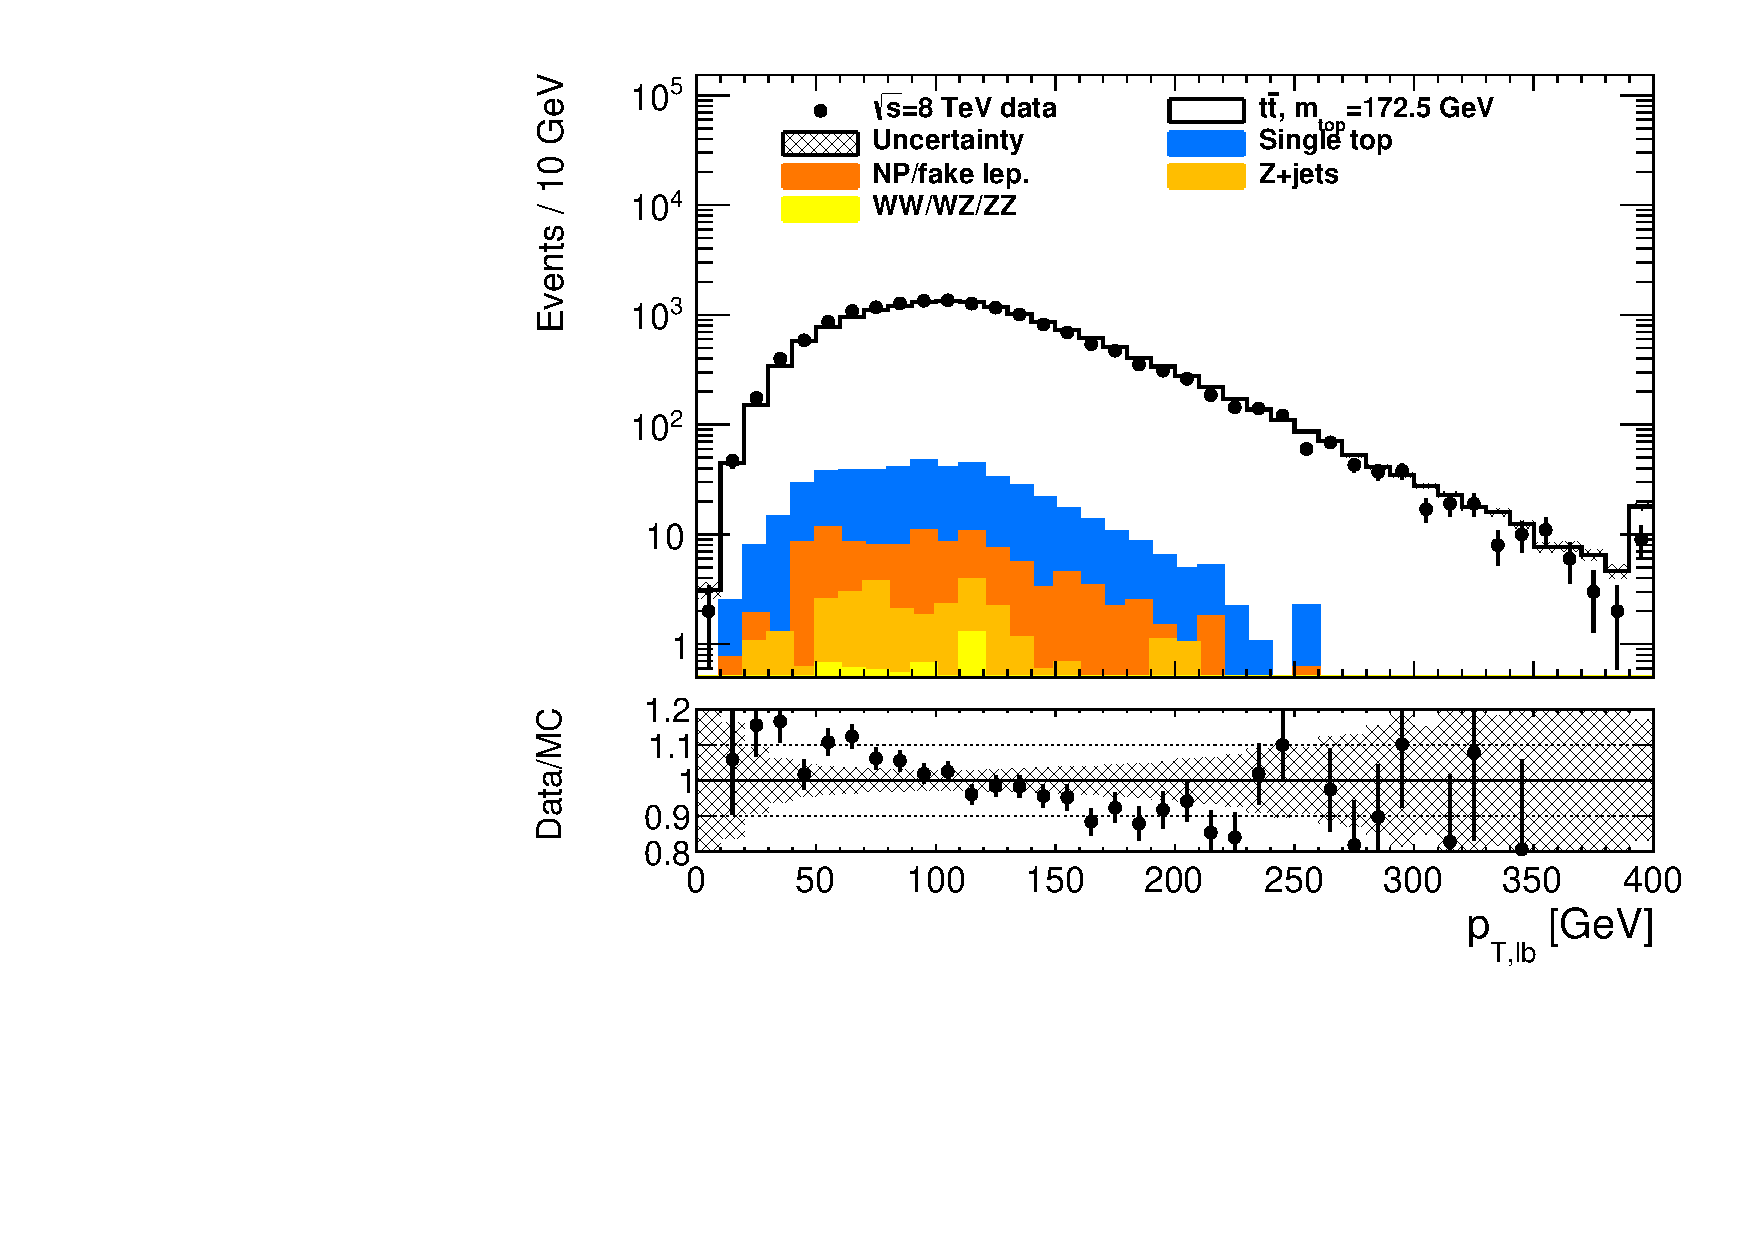
\includegraphics[width=0.49\textwidth]{./figs/fig_8TeV_TRC28_wp70_BDT-0.03/Dilep_SgnBkg_ratio_norm_sel3_ptlb_logscale.pdf}
  \label{sfig:ptlb_8TeV_mvabased}
}
\subfloat[\Mvabased]{
% \subfloat[$\dR_{\ell b}$]{
  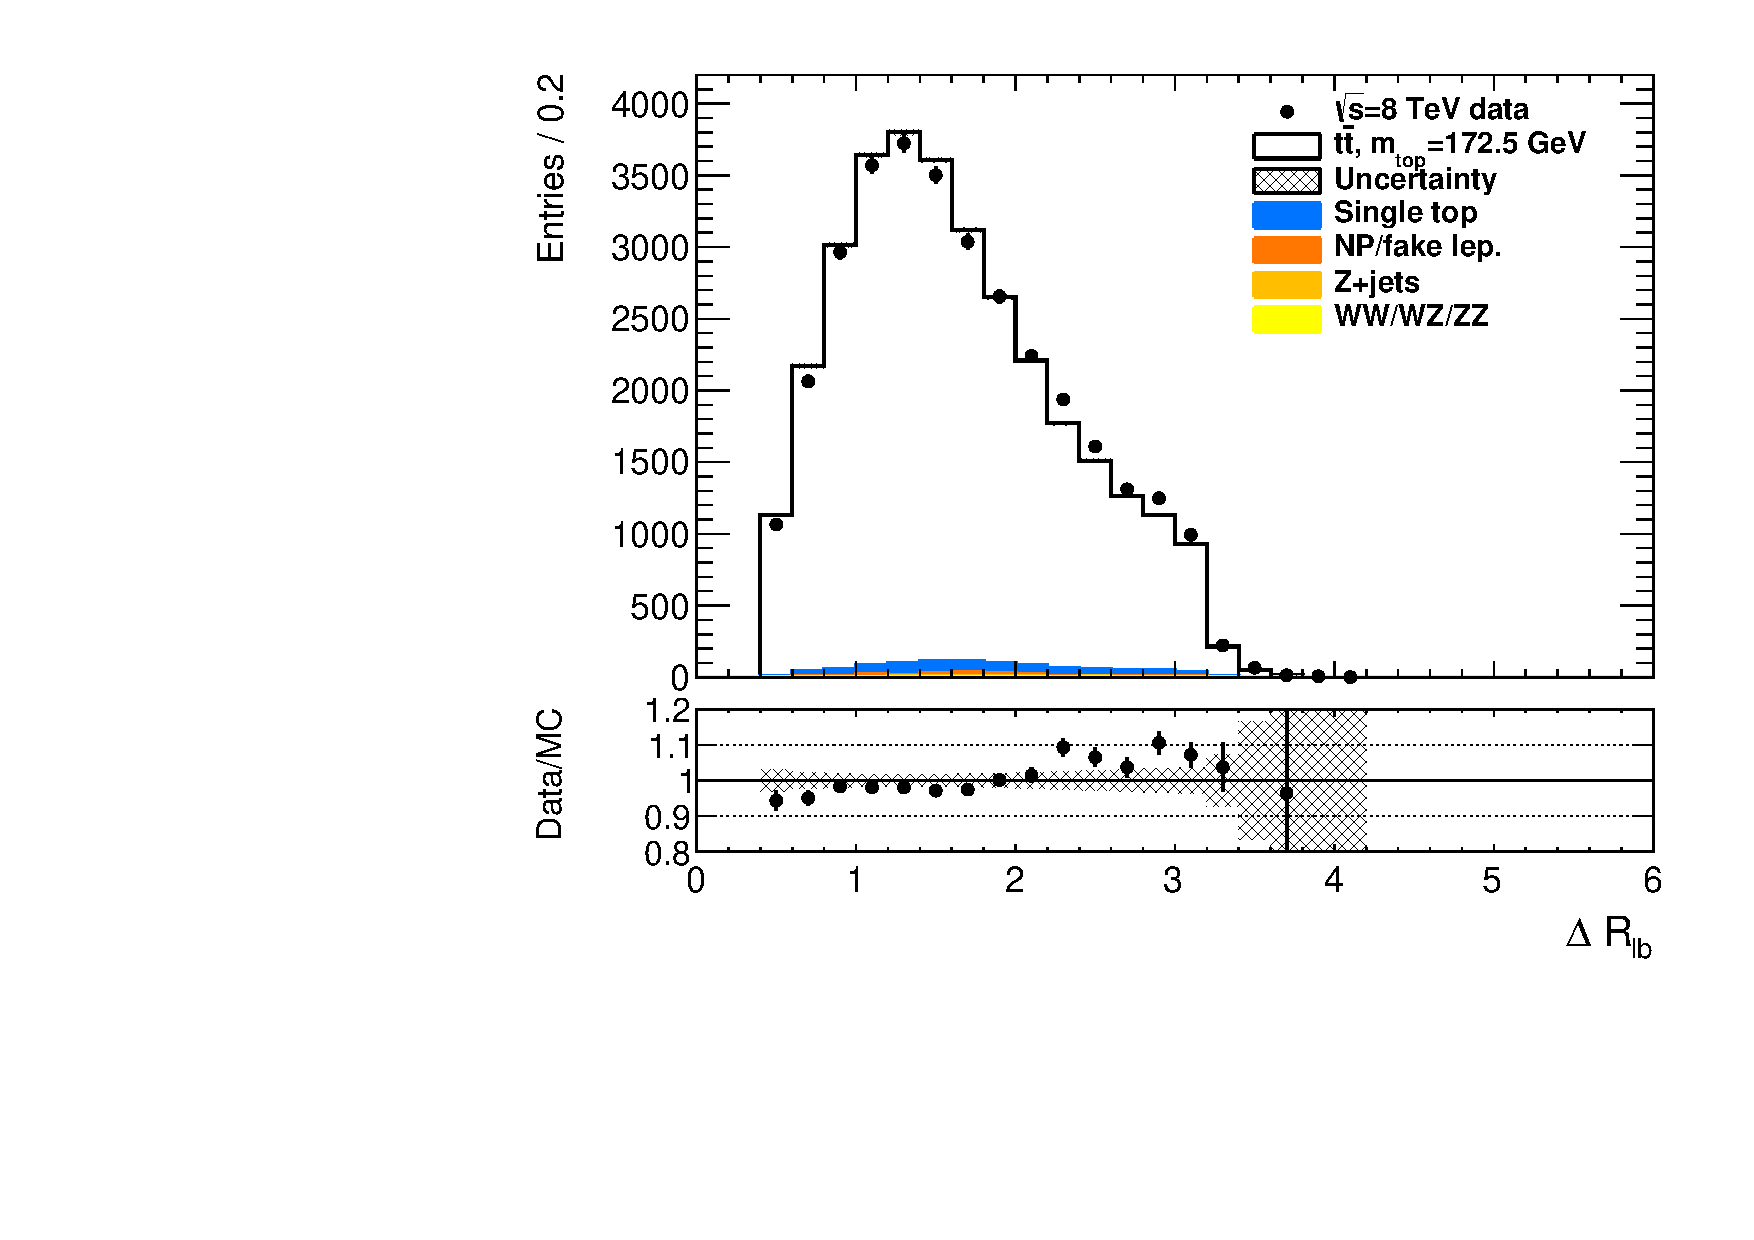
\includegraphics[width=0.49\textwidth]{./figs/fig_8TeV_TRC28_wp70_BDT-0.03/Dilep_SgnBkg_ratio_norm_sel3_dR_lb.pdf}
  \label{sfig:dR_lb_8TeV_mvabased}
}
%
% \caption[Data to \gls{MC} comparison for $\sqrts=8$~\TeV\ data]{
\caption[Data to \gls{MC} comparison for $\sqrts=8$~\TeV\ data: \ptlb\ and $\dR_{\ell b}$]{
%
Same as \fig~\ref{fig:DL_dataMC_njets} but showing the average \pt\ of the lepton--\bjet\ systems \ptlb\ on the left and the spatial distance of the lepton with respect to its matched \bjet\ $\dR_{\ell b}$ on the right.
%
\label{fig:DL_dataMC_lb}}
\end{figure*}
%%%%%%%%%%%%%%%%%%%%%%%%%%%%%%%%%%%%%%%%%%%%%%%%%%%%%%%%%%%%%%%%%%%%%%%%%%%%%
%
%
% %%%%%%%%%%%%%%%%%%%%%%%%%%%%%%%%%%%%%%%%%%%%%%%%%%%%%%%%%%%%%%%%%%%%%%%%%%%%%%%
% \begin{figure*}[tbp!]
% \centering
% \subfloat[Standard]{
% % \subfloat[\btagged\ jet $\eta$]{
%   \includegraphics[width=0.49\textwidth]{./figs/fig_8TeV_TRC28_wp70/Dilep_SgnBkg_ratio_norm_sel3_bJet_Eta.pdf}
%   \label{sfig:bJet_Eta_8TeV_standard}
% }
% \subfloat[Standard]{
% % \subfloat[Lepton $\eta$]{
%   \includegraphics[width=0.49\textwidth]{./figs/fig_8TeV_TRC28_wp70/Dilep_SgnBkg_ratio_norm_sel3_Lep_Eta.pdf}
%   \label{sfig:Lep_Eta_8TeV_standard}
% }
% \hfill
% \subfloat[\Cutbased]{
% % \subfloat[\btagged\ jet $\eta$]{
%   \includegraphics[width=0.49\textwidth]{./figs/fig_8TeV_TRC28_wp70_ptlb130/Dilep_SgnBkg_ratio_norm_sel3_bJet_Eta.pdf}
%   \label{sfig:bJet_Eta_8TeV_cutbased}
% }
% \subfloat[\Cutbased]{
% % \subfloat[Lepton $\eta$]{
%   \includegraphics[width=0.49\textwidth]{./figs/fig_8TeV_TRC28_wp70_ptlb130/Dilep_SgnBkg_ratio_norm_sel3_Lep_Eta.pdf}
%   \label{sfig:Lep_Eta_8TeV_cutbased}
% }
% \hfill
% \subfloat[\Mvabased]{
% % \subfloat[\btagged\ jet $\eta$]{
%   \includegraphics[width=0.49\textwidth]{./figs/fig_8TeV_TRC28_wp70_BDT-0.03/Dilep_SgnBkg_ratio_norm_sel3_bJet_Eta.pdf}
%   \label{sfig:bJet_Eta_8TeV_mvabased}
% }
% \subfloat[\Mvabased]{
% % \subfloat[Lepton $\eta$]{
%   \includegraphics[width=0.49\textwidth]{./figs/fig_8TeV_TRC28_wp70_BDT-0.03/Dilep_SgnBkg_ratio_norm_sel3_Lep_Eta.pdf}
%   \label{sfig:Lep_Eta_8TeV_mvabased}
% }
% %
% % \caption[Data to \gls{MC} comparison for $\sqrts=8$~\TeV\ data]{
% \caption[Data to \gls{MC} comparison for $\sqrts=8$~\TeV\ data: $\eta$]{
% %
% Same as \fig~\ref{fig:DL_dataMC_njets} but showing the \bjet\ $\eta$ distributions on the left and lepton $\eta$ distributions on the right.
% %
% \label{fig:DL_dataMC_eta}}
% \end{figure*}
% %%%%%%%%%%%%%%%%%%%%%%%%%%%%%%%%%%%%%%%%%%%%%%%%%%%%%%%%%%%%%%%%%%%%%%%%%%%%%
%
% %%%%%%%%%%%%%%%%%%%%%%%%%%%%%%%%%%%%%%%%%%%%%%%%%%%%%%%%%%%%%%%%%%%%%%%%%%%%%%%
\begin{figure*}[tbp!]
\centering
\subfloat[Standard]{
% \subfloat[\mlbr]{
  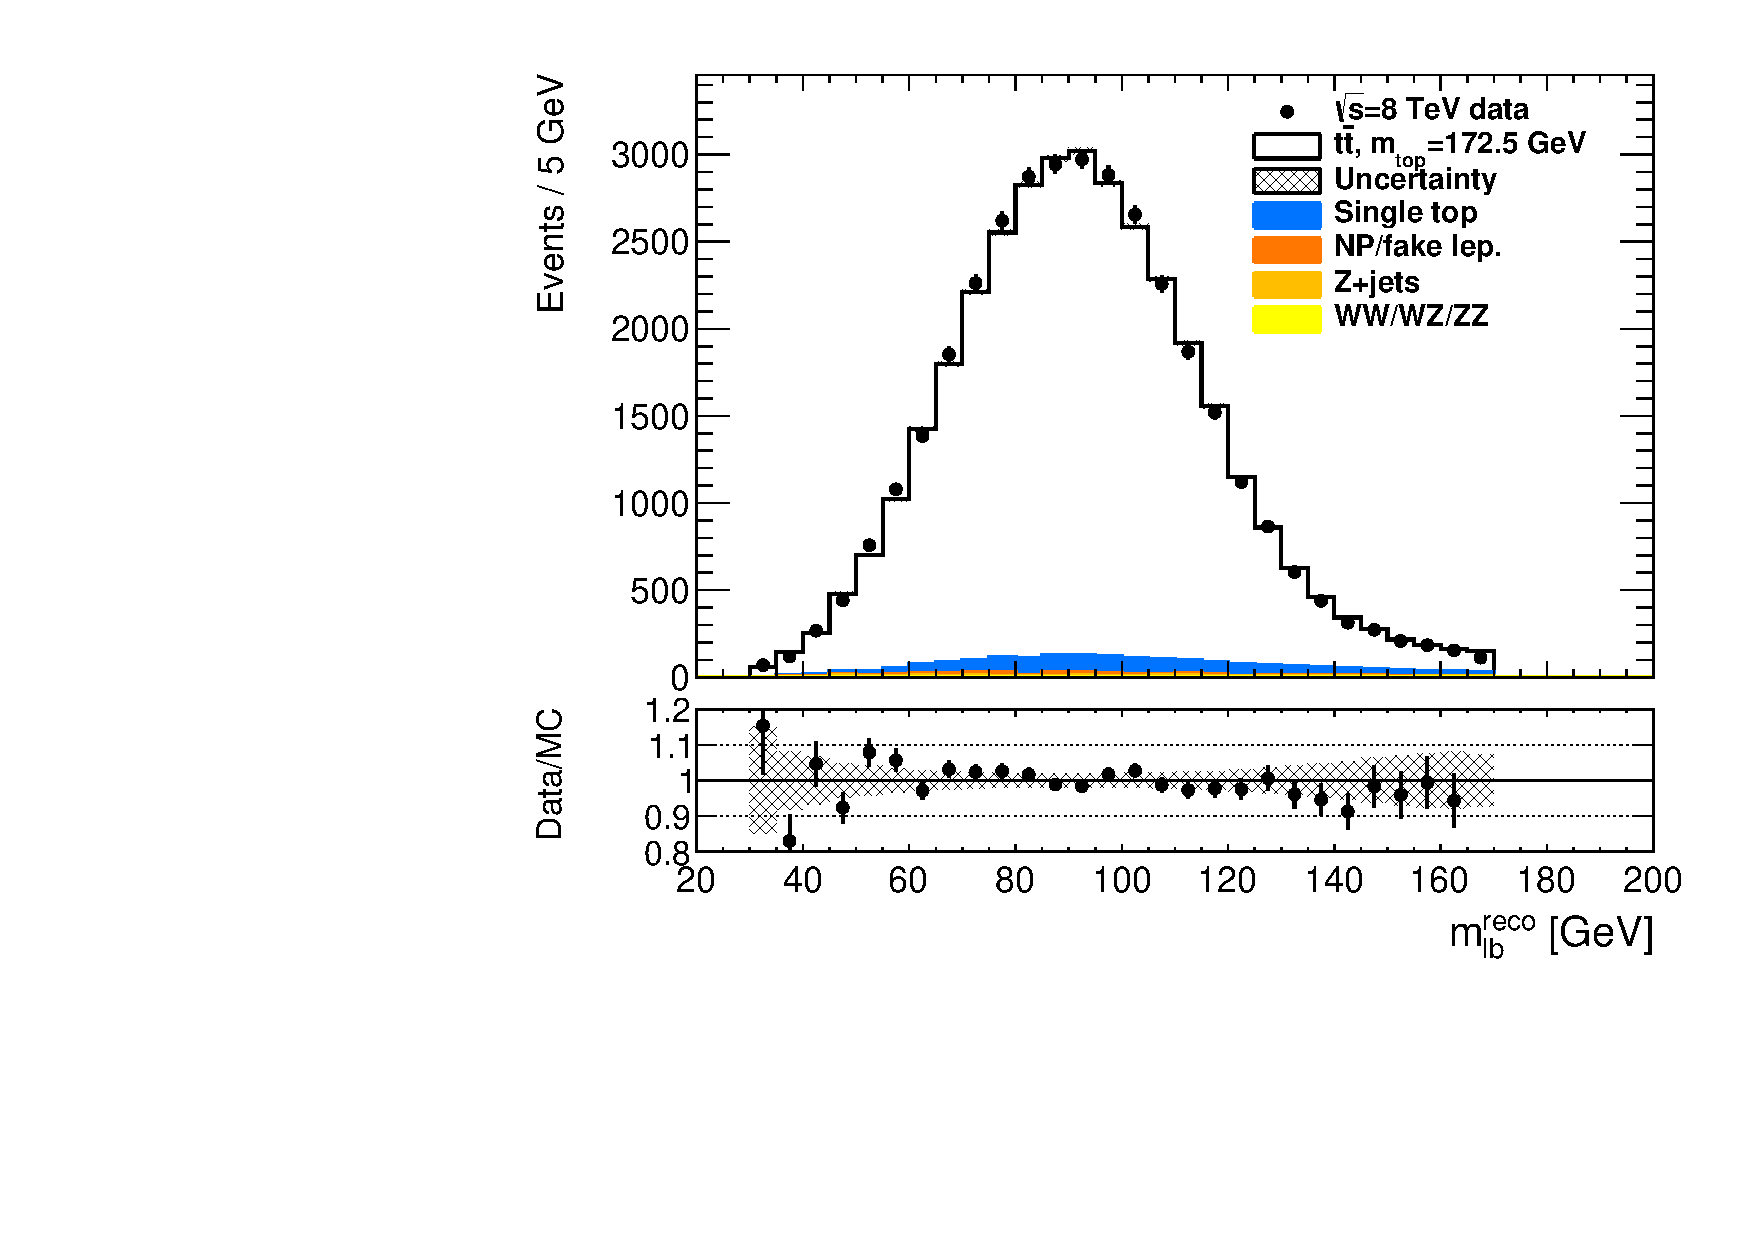
\includegraphics[width=0.55\textwidth]{./figs/fig_8TeV_TRC28_wp70/Dilep_SgnBkg_ratio_norm_sel3_mlb.pdf}
\label{sfig:mlb_8TeV_standard}
}
\hfill
\subfloat[\Cutbased]{
% \subfloat[\mlbr]{
  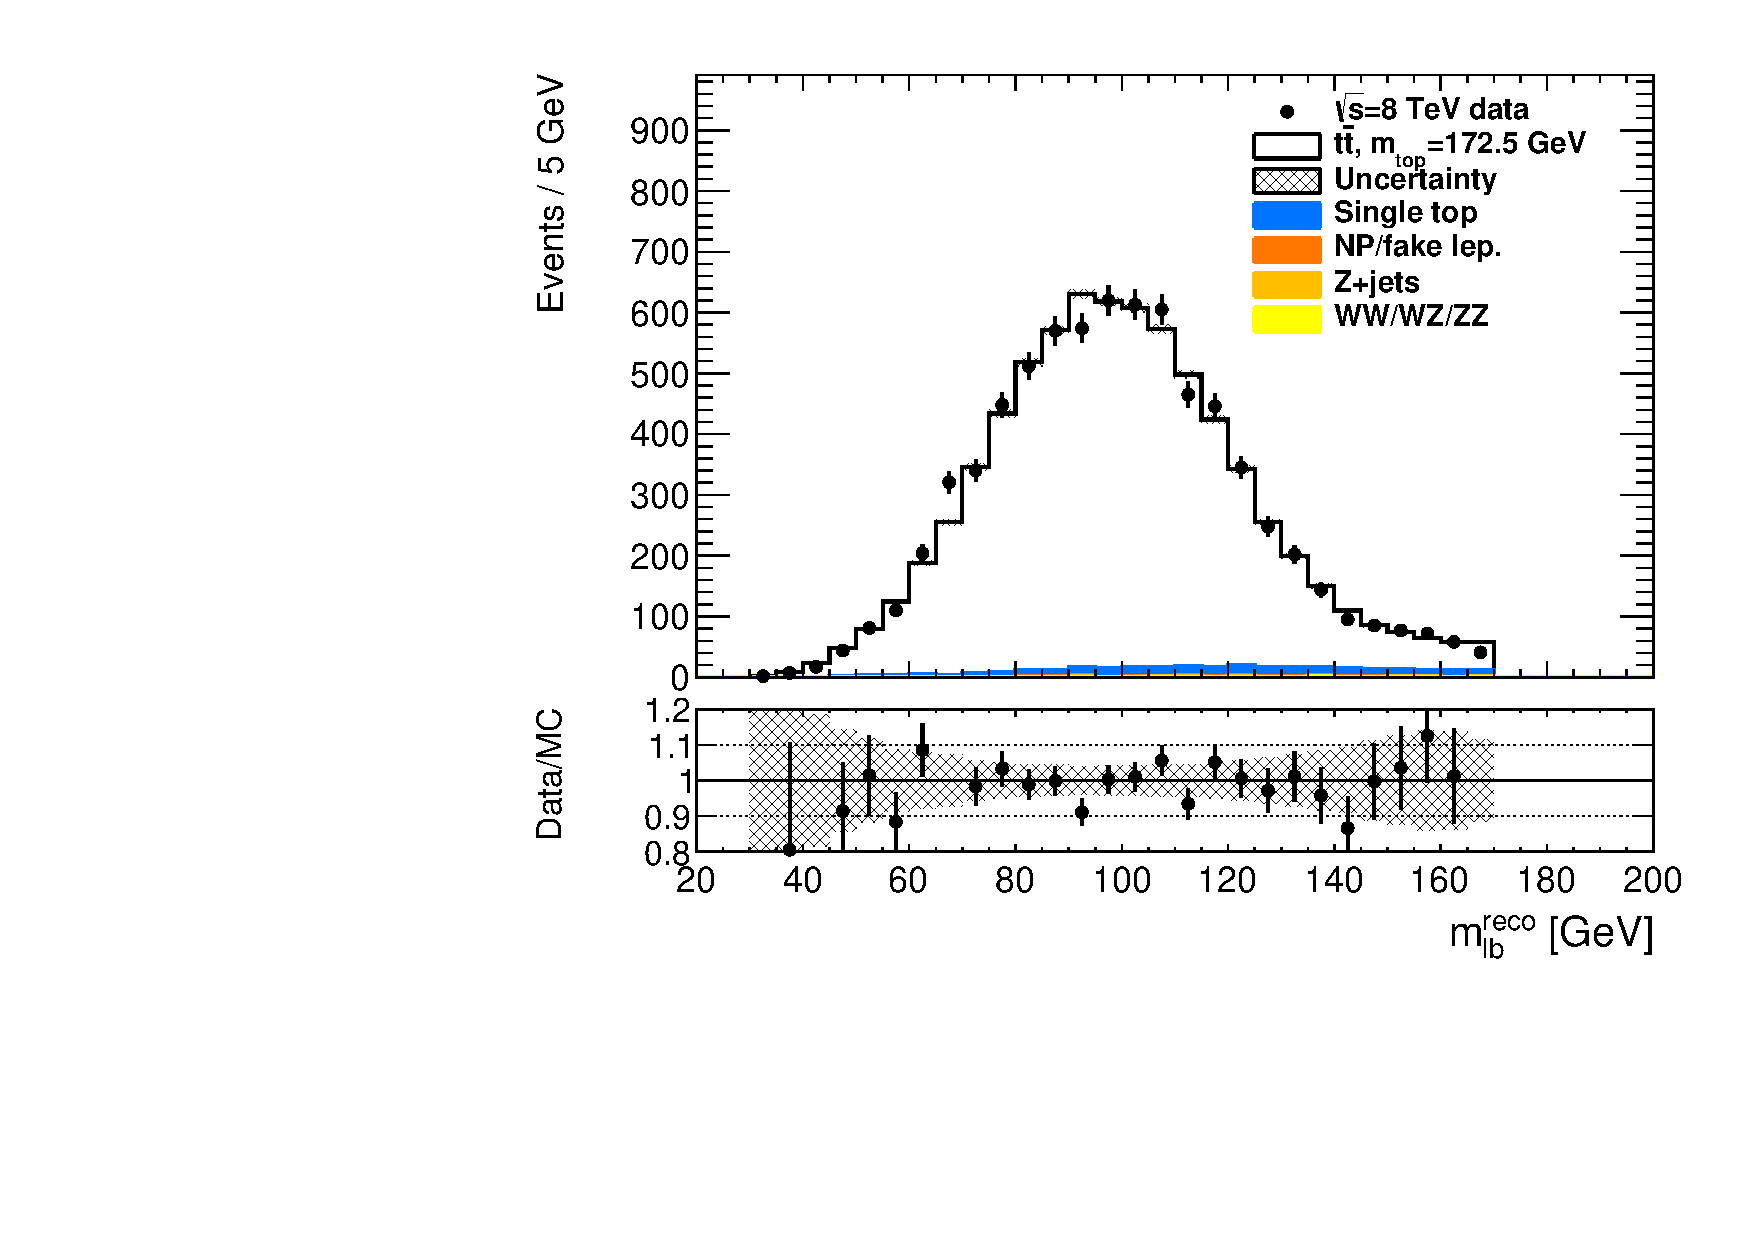
\includegraphics[width=0.55\textwidth]{./figs/fig_8TeV_TRC28_wp70_ptlb130/Dilep_SgnBkg_ratio_norm_sel3_mlb.pdf}
\label{sfig:mlb_8TeV_cutbased}
}
\hfill
\subfloat[\Mvabased]{
% \subfloat[\mlbr]{
  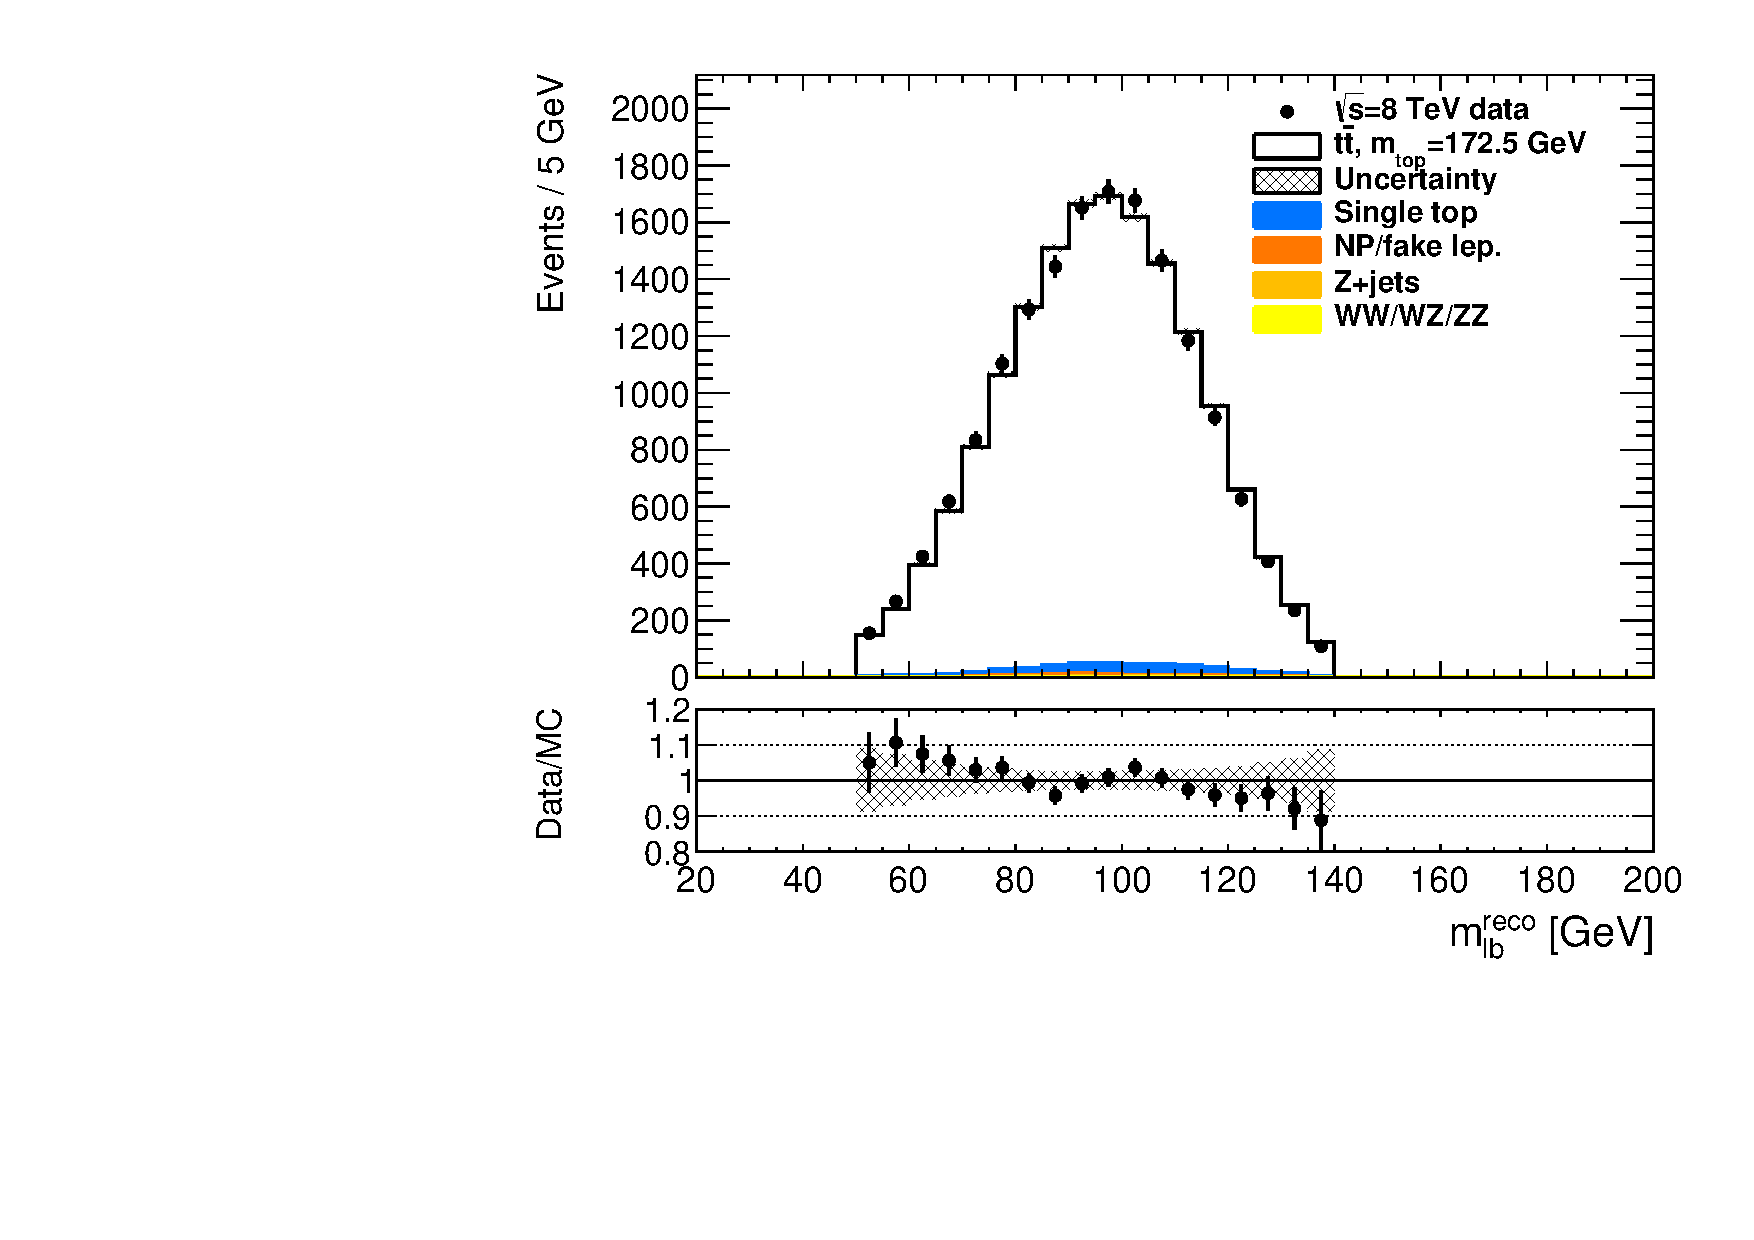
\includegraphics[width=0.55\textwidth]{./figs/fig_8TeV_TRC28_wp70_BDT-0.03/Dilep_SgnBkg_ratio_norm_sel3_mlb.pdf}
\label{sfig:mlb_8TeV_mvabased}
}
%
% \caption[Data to \gls{MC} comparison for $\sqrts=8$~\TeV\ data]{
\caption[Data to \gls{MC} comparison for $\sqrts=8$~\TeV\ data: \mlbr]{
%
Same as \fig~\ref{fig:DL_dataMC_njets} but showing the estimator distribution of \mlbr. The distributions have different ranges due to the selection specific restriction on \mlbr.
%
\label{fig:DL_dataMC_mlb}}
\end{figure*}
%%%%%%%%%%%%%%%%%%%%%%%%%%%%%%%%%%%%%%%%%%%%%%%%%%%%%%%%%%%%%%%%%%%%%%%%%%%%%
%

% %
% %%%%%%%%%%%%%%%%%%%%%%%%%%%%%%%%%%%%%%%%%%%%%%%%%%%%%%%%%%%%%%%%%%%%%%%%%%%%%%%
% % \begin{figure*}[h!]
% \begin{figure*}[tbp!]
% \centering
% % \subfloat[\mlbr\ for exactly two \btagged\ jets]{
% 	\includegraphics[width=0.5\textwidth]{./figs/LHC8-P_Tavt-norm.eps}
% 	% \label{sfig:mlbrmtop}
% % }
% \caption[NNLO prediction for the \tquark\ \pt]{
% %
% Normalised \tquark\ \pt\ distributions at different order in \gls{QCD}~\cite{Czakon:2015owf} in comparison to \gls{CMS} data from the \ljets\ \ttbar\ decay channel at $\sqrts=8$~\TeV~\cite{Khachatryan:2015oqa}.
% %
% \label{fig:NNLOtoppt}}
% \end{figure*}
% %%%%%%%%%%%%%%%%%%%%%%%%%%%%%%%%%%%%%%%%%%%%%%%%%%%%%%%%%%%%%%%%%%%%%%%%%%%%%
% %

\clearpage


















\section{The template fit}
\label{sec:templates8TeV}
%
%
%%%%%%%%%%%%%%%%%%%%%%%%%%%%%%%%%%%%%%%%%%%%%%%%%%%%%%%%%%%%%%%%%%%%%%%%%%%%%%%%%%%%%%
\begin{figure*}[tbp!]
\centering
\subfloat[Signal templates]{
  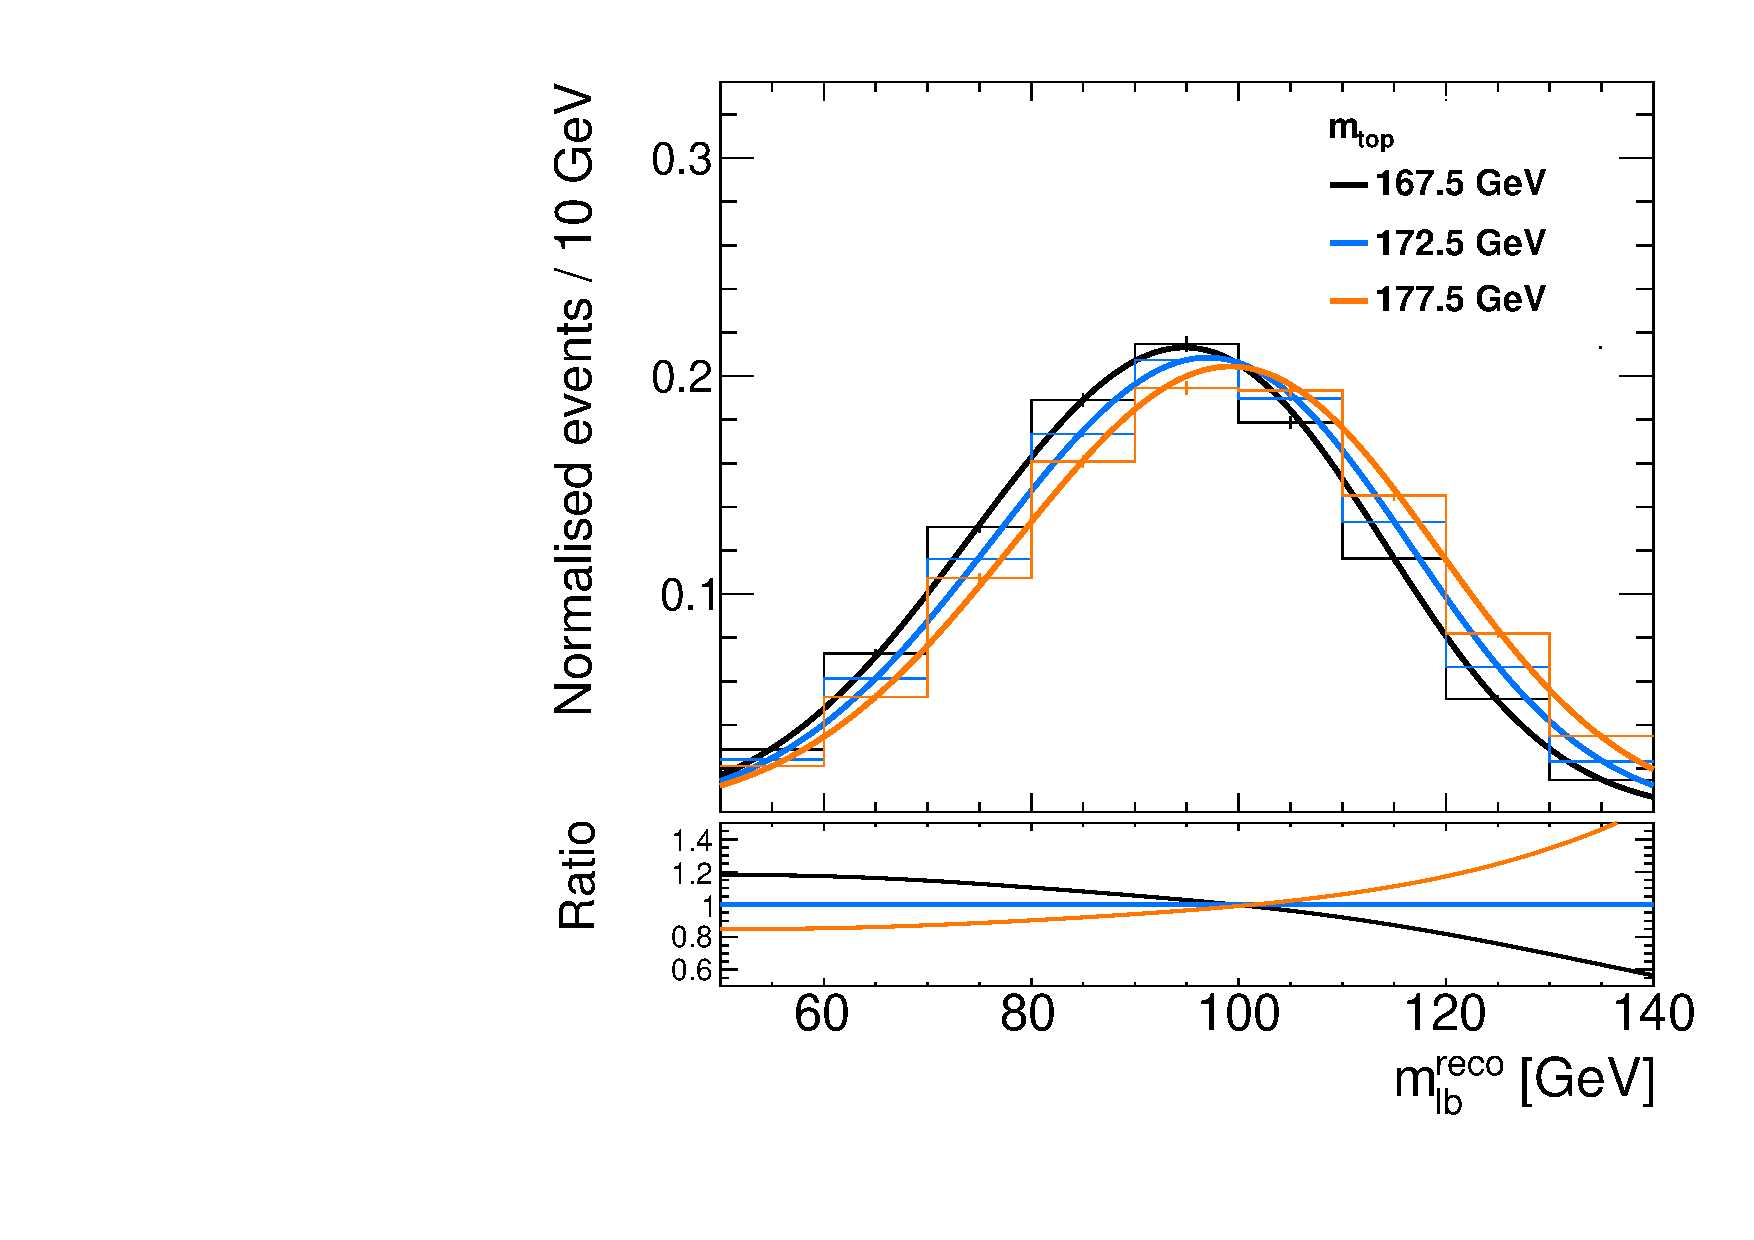
\includegraphics[width=0.49\textwidth]{./figs/fig_8TeV_TRC28_wp70_BDT-0.03/mlb_fit_all_doublegauss_shift_sel3.pdf}
  \label{sfig:sigtmpl}
}
\subfloat[Background template]{
  \includegraphics[width=0.49\textwidth]{./figs/fig_8TeV_TRC28_wp70_BDT-0.03/mlb_BkgFit_shift_withfunc_sel3.pdf}
  \label{sfig:bkgtmpl}
}
\caption[Template fit functions for $\sqrts=8$~\TeV\ data]{
%
The templates of the \mvabased\ analysis for~\subref{sfig:sigtmpl} the signal for different values of \mt\ and~\subref{sfig:bkgtmpl} the background contribution.
%
The corresponding \glspl{pdf} are displayed on top of the distributions and their ratios are drawn below.
%
The uncertainty bars are statistical only.
%
\label{fig:tmpl8TeV}}
\end{figure*}
%%%%%%%%%%%%%%%%%%%%%%%%%%%%%%%%%%%%%%%%%%%%%%%%%%%%%%%%%%%%%%%%%%%%%%%%%%%%%%%%%%%%%%
%
The signal templates are constructed as a function of the \tquark\ mass used in the \gls{MC} generator in the range $167.5$ to $177.5$~\GeV\ in steps of $2.5$~\GeV, using separate samples for each of the five different mass points.
%
They comprise both the \ttbar\ and the single top quark production processes. The sum of a Gaussian and a Landau in the standard and the \cutbased, and the sum of two Gaussian functions in the \mvabased\ analysis are found to give a good description of the distribution shape. 
%
Since the single \tquark\ contribution is accounted for in the signal templates, the background distribution does not vary as a function of \mt. A Gaussian function is fitted to the background distribution.
%
The superposition of the signal templates and the corresponding fitted \glspl{pdf} for three \mt\ values is shown in \fig~\ref{fig:tmpl8TeV}. The background template with its fitted \gls{pdf} is shown as well. These and all subsequent figures are taken from the \mvabased\ analysis. 

%
%%%%%%%%%%%%%%%%%%%%%%%%%%%%%%%%%%%%%%%%%%%%%%%%%%%%%%%%%%%%%%%%%%%%%%%%%%%%%%%%%%%%%%
\begin{figure*}[tbp!]
\centering
\subfloat[\mt\ residual]{
  % \includegraphics[width=0.49\textwidth]{./figs/fig_8TeV_TRC28_wp70_ptlb130/{mlb_Pexp_langauss_shape0_bkgfr0.010_pe1000_invpb20277_seed2_sel3_massdiff}.pdf}
  \includegraphics[width=0.49\textwidth]{./figs/fig_8TeV_TRC28_wp70_BDT-0.03/{mlb_Pexp_doublegauss_shape0_bkgfr0.010_pe1000_invpb20277_seed5_sel3_massdiff}.pdf}
  \label{sfig:bias8TeV}
}
\subfloat[Pull mean]{
  % \includegraphics[width=0.49\textwidth]{./figs/fig_8TeV_TRC28_wp70_ptlb130/{mlb_Pexp_langauss_shape0_bkgfr0.010_pe1000_invpb20277_seed2_sel3_pull_mean}.pdf}
  \includegraphics[width=0.49\textwidth]{./figs/fig_8TeV_TRC28_wp70_BDT-0.03/{mlb_Pexp_doublegauss_shape0_bkgfr0.010_pe1000_invpb20277_seed5_sel3_pull_mean}.pdf}
  \label{sfig:pullmean8TeV}
}
\hfill
\subfloat[Pull width]{
  % \includegraphics[width=0.49\textwidth]{./figs/fig_8TeV_TRC28_wp70_ptlb130/{mlb_Pexp_langauss_shape0_bkgfr0.010_pe1000_invpb20277_seed2_sel3_pull_width}.pdf}
  \includegraphics[width=0.49\textwidth]{./figs/fig_8TeV_TRC28_wp70_BDT-0.03/{mlb_Pexp_doublegauss_shape0_bkgfr0.010_pe1000_invpb20277_seed5_sel3_pull_width}.pdf}
  \label{sfig:pullwidth8TeV}
}
\subfloat[Observed statistical uncertainty]{
  % \includegraphics[width=0.49\textwidth]{./figs/fig_8TeV_TRC28_wp70_ptlb130/{mlb_Pexp_langauss_shape0_bkgfr0.010_pe1000_invpb20277_seed2_sel3_error}.pdf}
  \includegraphics[width=0.49\textwidth]{./figs/fig_8TeV_TRC28_wp70_BDT-0.03/{mlb_Pexp_doublegauss_shape0_bkgfr0.010_pe1000_invpb20277_seed5_sel3_error}.pdf}
  \label{sfig:stat8TeV}
}
\hfill
\subfloat[Distribution for $\mt=172.5$~\GeV\ of the observed statistical uncertainty]{
  % \includegraphics[width=0.49\textwidth]{./figs/fig_8TeV_TRC28_wp70_ptlb130/{mlb_Pexp_langauss_shape0_bkgfr0.010_pe1000_invpb20277_seed2_sel3_staterrordistr}.pdf}
  \includegraphics[width=0.49\textwidth]{./figs/fig_8TeV_TRC28_wp70_BDT-0.03/{mlb_Pexp_doublegauss_shape0_bkgfr0.010_pe1000_invpb20277_seed5_sel3_expstaterr}.pdf}
  \label{sfig:expstat8TeV}
}
\caption[\mt\ residual and pull distributions for $\sqrts=8$~\TeV\ data]{
%
\Fig~\subref{sfig:bias8TeV} shows the \mt\ residuals observed when applying the method to the respective input templates. \Fig{s}~\subref{sfig:pullmean8TeV} and \subref{sfig:pullwidth8TeV} show the pull distribution mean and width. 
%
The dashed lines correspond to the expected values of zero and one respectively. The full lines are the result of a fit of a constant to the points. 
%
\Fig~\subref{sfig:stat8TeV} shows the observed statistical uncertainty as a function of \mt, representing the mean and width parameters of fits with Gaussian functions to the distributions of the observed statistical uncertainty, as the one for $\mt=172.5$~\GeV, shown in \fig~\subref{sfig:expstat8TeV}.
%
\label{fig:pull8TeV}}
\end{figure*}
%%%%%%%%%%%%%%%%%%%%%%%%%%%%%%%%%%%%%%%%%%%%%%%%%%%%%%%%%%%%%%%%%%%%%%%%%%%%%%%%%%%%%%
%
The likelihood to be maximised is the same as specified in \sect~\ref{sect:like7TeV} but for the fact that the background contribution is fixed in the fit to the expected value of \bkgfrBDT\ for all analyses.
%and \bkgfrEightTeV\ for the \mvabased and \cutbased\ analysis, respectively.
%%%%%%%%%%%%%%%%%%%%%%%%%%%%%%%%%%%%%%%%%%%%%%%%%%%%%%%%%%%%%%%%%%%%%%%%%%%%%%%
\begin{equation*}
%
\Like(\mt) = 
\prod_{i=1}^{N} 
\left[ (1-\fbkg)\cdot \Ptopsig(\mlbri \,\vert\, \mt) + \fbkg \cdot \Ptopbkg(\mlbri) \right]
%
% \label{eq:LikeDL7TeV}
\end{equation*}
%%%%%%%%%%%%%%%%%%%%%%%%%%%%%%%%%%%%%%%%%%%%%%%%%%%%%%%%%%%%%%%%%%%%%%%%%%%%%%%
%
In contrast to the $\sqrts=7$~\TeV\ analyses, where the likelihood functions for the samples containing one or two \bjet{s} have been treated independently and only combined at likelihood level, the analyses at $\sqrts=8$~\TeV\ use a single likelihood for all selected events. %The statistical uncertainty is taken from the parabolic approximation of the likelihood profile. %mentioned below anyway
%
Pseudo-experiments are used to verify the internal consistency of the fitting procedure.
%
These pseudo-experiments are performed 1000 times per mass point and corrected for oversampling~\cite{BarlowCF}. No significant deviation is found between the input parameters and the results of the fits, proving that the estimator has no bias. The \mt\ residuals, the pull and the expected statistical uncertainty distributions are shown in \fig~\ref{fig:pull8TeV}.
%
The residuals and pull means are consistent with zero within the uncertainties. A fit with a first order polynomial shows non-significant slope, and the offset obtained from a fit of a constant is assigned as the method calibration uncertainty. 
%
% The pull widths are consistent with one for all \mt\ values. The statistical uncertainty on the determination of \mt\ is increasing with \mt, showing that larger masses have a slightly worse resolution.
The pull widths are consistent with one for all \mt\ values within one or two standard deviations. The statistical uncertainty on the determination of \mt\ is not significantly increasing with \mt, showing that the mass distributions have similar resolution.
%
In summary, these investigations show that the method is unbiased and the statistical uncertainty is evaluated correctly.
%
The distribution of statistical uncertainties for $\mt=172.5$~\GeV\ is approximately Gaussian in shape and a fit of a Gaussian function yields expected statistical uncertainties of \ExpstatuncStandard, $\ExpstatuncEight\pm\ExpstatuncEightunc$ and \ExpstatuncBDT~\GeV\ for the standard, the \cutbased\ and \mvabased\ analysis, respectively.





















%
%%%%%%%%%%%%%%%%%%%%%%%%%%%%%%%%%%%%%%%%%%%%%%%%%%%%%%%%%%%%%%%%%%%%%%%%%%%%%%%%%%%%%%
\begin{figure*}[tbp!]
\centering
\subfloat[Standard]{
  % \includegraphics[height=0.48\textwidth]{./figs/fig_8TeV_TRC28_wp70/{mlb_fit_f1_m0_full_invpb20276_bkgfr0.010_sel3_main}.pdf}
  \includegraphics[height=0.39\textwidth]{./figs/fig_8TeV_TRC28_wp70/{mlb_fit_f1_m0_full_invpb20276_bkgfr0.010_sel3_main}.pdf}
  \label{sfig:result8TeVstandard}
}
\subfloat[Standard]{
  % \includegraphics[height=0.48\textwidth]{./figs/fig_8TeV_TRC28_wp70/{mlb_fit_f1_m0_full_invpb20276_bkgfr0.010_sel3_like}.pdf}
  \includegraphics[height=0.39\textwidth]{./figs/fig_8TeV_TRC28_wp70/{mlb_fit_f1_m0_full_invpb20276_bkgfr0.010_sel3_like}.pdf}
  \label{sfig:like8TeVstandard}
}
\hfill
\subfloat[\Cutbased]{
  % \includegraphics[height=0.48\textwidth]{./figs/fig_8TeV_TRC28_wp70_ptlb130/{mlb_fit_f1_m0_full_invpb20276_bkgfr0.010_sel3_main}.pdf}
  \includegraphics[height=0.39\textwidth]{./figs/fig_8TeV_TRC28_wp70_ptlb130/{mlb_fit_f1_m0_full_invpb20276_bkgfr0.010_sel3_main}.pdf}
  \label{sfig:result8TeVcut}
}
\subfloat[\Cutbased]{
  % \includegraphics[height=0.48\textwidth]{./figs/fig_8TeV_TRC28_wp70_ptlb130/{mlb_fit_f1_m0_full_invpb20276_bkgfr0.010_sel3_like}.pdf}
  \includegraphics[height=0.39\textwidth]{./figs/fig_8TeV_TRC28_wp70_ptlb130/{mlb_fit_f1_m0_full_invpb20276_bkgfr0.010_sel3_like}.pdf}
  \label{sfig:like8TeVcut}
}
\hfill
\subfloat[\Mvabased]{
  % \includegraphics[height=0.48\textwidth]{./figs/fig_8TeV_TRC28_wp70_BDT-0.03/{mlb_fit_f1_m0_full_invpb20276_bkgfr0.010_sel3_main}.pdf}
  \includegraphics[height=0.39\textwidth]{./figs/fig_8TeV_TRC28_wp70_BDT-0.03/{mlb_fit_f1_m0_full_invpb20276_bkgfr0.010_sel3_main}.pdf}
  \label{sfig:result8TeVmva}
}
\subfloat[\Mvabased]{
  % \includegraphics[height=0.48\textwidth]{./figs/fig_8TeV_TRC28_wp70_BDT-0.03/{mlb_fit_f1_m0_full_invpb20276_bkgfr0.010_sel3_like}.pdf}
  \includegraphics[height=0.39\textwidth]{./figs/fig_8TeV_TRC28_wp70_BDT-0.03/{mlb_fit_f1_m0_full_invpb20276_bkgfr0.010_sel3_like}.pdf}
  \label{sfig:like8TeVmva}
}
\caption[Likelihood fit for $\sqrts=8$~\TeV\ data]{
%
\Fig{s}~\subref{sfig:result8TeVstandard}, \subref{sfig:result8TeVcut} and \subref{sfig:result8TeVmva} show the data distributions of \mlbr\ and the fitted \glspl{pdf} for the background alone and for signal-plus-background for the standard, the \cutbased\ and the \mvabased\ analysis, respectively. \Fig{s}~\subref{sfig:like8TeVstandard}, \subref{sfig:like8TeVcut} and \subref{sfig:like8TeVmva} display the corresponding likelihood profiles as a function of \mt.
%
\label{fig:result8TeV}}
\end{figure*}
%%%%%%%%%%%%%%%%%%%%%%%%%%%%%%%%%%%%%%%%%%%%%%%%%%%%%%%%%%%%%%%%%%%%%%%%%%%%%%%%%%%%%%
%



%%%%%%%%%%%%%%%%%%%%%%%%%%%%%%%%%%%%%%%%%%%%%%%%%%%%%%%%%%%%%%%%%%%%%%%%%%%%%%%%
\begin{table}[tbp!]
\setlength{\belowcaptionskip}{-0.3cm}
% \footnotesize
\begin{center}
\begin{tabular}{|l|c|c|c|c|c|c|c|c|c|}
\cline{5-10}
%
% \multicolumn{3}{c|}{}                                 & \multicolumn{3}{c|}{Correlation $\rho$} & \multicolumn{3}{c|}{Deviation [$\sigma_\rho$] ($\sigma_\rho$ [\GeV])} \\ \hline
% Selection & Events    & $\sigma^*$ [\GeV] & Std.     & Cut       & \mvabased        & Std.         & Cut            & \mvabased   \\ \hline
% Standard  & $35099$   &          $0.22$               & $  1   $ & $ 0.59  $ & $  0.79 $        & $  0 ~(0)   $ & $ 1.22~ (0.38) $ & $ 1.76 ~(0.20)  $   \\
% \Cutbased & $ 7346$   &          $0.48$               & $      $ & $   1   $ & $  0.69 $        & $          $ & $   0  ~(0   ) $ & $ 2.39 ~(0.34)  $   \\
% \mvabased & $16117$   &          $0.32$               & $      $ & $       $ & $   1   $        & $          $ & $             $ & $   0  ~(0   )  $   \\ \hline
%
\multicolumn{4}{c|}{}                     & \multicolumn{3}{c|}{Correlation $\rho$} & \multicolumn{3}{c|}{Significance [$\sigma$]} \\ \hline
Selection & Events   & Fraction         & $\sigma^*$ [\GeV] & Std.     & Cut       & \mvabased & Std.     & Cut      & \mvabased   \\ \hline
Standard  & $35099$  & $100\%$          & $0.22$            & $1$      & $ 0.59 $  & $ 0.79 $  & $  0   $ & $ 1.22 $ & $ 1.76  $   \\
\Cutbased & $ 7346$  & \OptiFraction    & $0.48$            & $ $      & $   1  $  & $ 0.69 $  & $      $ & $   0  $ & $ 2.39  $   \\
\mvabased & $16117$  & \BDTOptiFraction & $0.32$            & $ $      & $      $  & $  1   $  & $      $ & $      $ & $   0   $   \\ \hline
\end{tabular}
\end{center}
\vspace{-0.4cm}
\caption[Selection efficiency at \truelevel]{
%
The numbers of data events in the respective selections and the extrapolated statistical uncertainty $\sigma^*$, obtained from scaling the statistical uncertainty of the standard selection by the square-root of the event fraction.
%
The statistical correlation $\rho$ of the data samples $i$ and $j$ is given, determined as $\rho_{ij}=\sqrt{2\N{ij}/(\N{i}+\N{j})}$, as well as the statistical significance of the respective central value differences. 
%
\label{tab:8TeVdatacompat}
}
\end{table}
%%%%%%%%%%%%%%%%%%%%%%%%%%%%%%%%%%%%%%%%%%%%%%%%%%%%%%%%%%%%%%%%%%%%%%%%%%%%%%%%

\section{Result in the data}
\label{sect:application8TeV}
%
In what follows, the results of the fit to the data are blinded\footnote{Within \gls{ATLAS} before approval for publication, results are typically blinded to avoid comparison to existing results while optimising the analysis.} by applying a constant offset to the measured values of \mt. %comment for unblinded
%
The offset is drawn as random number from a Gaussian \gls{pdf} centred at zero and with a width according to the expected statistical uncertainty of the \cutbased\ analysis. The same offset is used for the three $\sqrts=8$~\TeV\ analyses to allow for investigation of their consistency. %comment for unblinded
%
\Fig~\ref{fig:result8TeV} shows the \mlbr\ distributions in the data together with the corresponding fitted \glspl{pdf} for the background alone and for the sum of signal and background. The corresponding likelihood profiles are shown as well.
%
% The uncertainty band shown is the envelope of all \glspl{pdf}, obtained from 1000 pseudo-experiments with fixed background fractions while varying the fitted parameters \mt\ within $\pm 1\sigma$ of its full uncertainties. 
%
% Within this band, the data are well described by the fitted probability density function.
%
The likelihood fits to the data yield
%
% %%%%%%%%%%%%%%%%%%%%%%%%%%%%%%%%%%%%%%%%%%%%%%%%%%%%%%%%%%%%%%%%%%%%%%%%%%%%%%%
\begin{eqnarray*}
  \mt^\mathrm{Standard} & = &\XZst{\EightValueStandard}{\EightStatStandard}~\GeV \\
  \mt^\mathrm{Cut}       & = &\XZst{\EightValue}{\EightStat}~\GeV \\
  \mt^\mathrm{\gls{BDT}} & = &\XZst{\BDTValue}{\BDTStat}~\GeV
\end{eqnarray*}
% %%%%%%%%%%%%%%%%%%%%%%%%%%%%%%%%%%%%%%%%%%%%%%%%%%%%%%%%%%%%%%%%%%%%%%%%%%%%%%%
%
for the standard, the \cutbased\ and the \mvabased\ analyses, with the background fractions fixed to the expectation of \bkgfrBDT\ 
% and \bkgfrEightTeV\ 
given in \tab~\ref{tab:selections}. 
%
The statistical uncertainties are taken from the parabolic approximation of the likelihood profiles.
%
As seen from comparison to \tab~\ref{tab:8TeVdatacompat}, the statistical precisions scale with the ratio of the square-root of numbers of events in the final event selections. The absence of a data-inherent difference in sensitivity beyond the purely statistical effect shows that the mass resolution remains untouched by the optimisation procedures.
%
The compatibility of results in terms of statistical uncertainty only is given in the table as well, where the statistical correlations of the data samples and the significances of the central value differences are reported.
%
%difference MVA and cut
The tension between the \cutbased\ and the \mvabased\ results is resolved when taking into account the systematic uncertainties and the corresponding correlations.
%
With the resulting total correlation of \BDTcutCorrelation, the results of the two optimised events selections are compatible at the level of \BDTcutCompatibility\ standard deviations. 
%
These systematic effects are discussed in the next section.









\section[Uncertainties affecting the \mt\ determination]{Uncertainties affecting the \boldmath$\mt$ determination}
\label{sect:unc8TeV}
%
The uncertainty determination procedure follows the one detailed in \sect~\ref{sect:unc7TeV}. For each systematic variation sample, 1000 pseudo-experiments are performed by drawing random entries from the corresponding templates. The restriction at $\sqrts=7$~\TeV\ to 500 pseudo-experiments was imposed for consistency with the \ttbarlj\ analysis, described in \sect~\ref{sec:resultcomb7TeV}, which was technically coupled to the \ttbarll\ analysis and posed higher computing demands. Both numbers of pseudo-experiments suffice for a precise determination of uncertainties. The statistical precision on the systematic uncertainties has been calculated as detailed in \sect~\ref{sect:syststat}. 
%
The statistical precision of the \mt\ determination in the systematically varied event samples ranges from less than $100$~\MeV\ for the central \ttbar\ sample to about $300$~\MeV\ for the samples with the lowest number of events.
%
Most estimations are based on the same sample with only a change in a single parameter, leading to a high correlation of the estimates of the central \mt\ values and a correspondingly low uncertainty on their difference. 
%
The resulting total uncertainty and all uncertainty components with their statistical precisions are listed in \tab~\ref{tab:llresults8TeV}.
%
%--------------------------------------------------------------------------
\begin{table*}[tb!]
%\footnotesize
\small
\begin{center}
\begin{tabular}{|l|r|r|r|r|}\cline{2-5}
\multicolumn{1}{c|}{}                &  \multicolumn{4}{c|}{\mt\ [\GeV]}  \\ \cline{2-5}
\multicolumn{1}{c|}{}                &  \multicolumn{3}{c|}{$\sqrts=8$~\TeV}                                                 &   $\sqrts=7$~\TeV\ \\ \hline
Event selecton                       &  Standard                      &  \Cutbased\            &  \Mvabased\                 &   Standard        \\ \hline
 Result  ($\sqrts=8$~\TeV\ blinded)  &  \EightValueStandard           &  \EightValue           &  \BDTValue                  &   173.79          \\ \hline%comment for unblinded
       Statistics                    &  \EightStatStandard            &  \EightStat            &  \BDTStat                   &     0.54          \\ \hline
           Method                    &  0.05 $\pm$ 0.04               &  0.11 $\pm$ 0.08       &  0.05 $\pm$ 0.06            &  0.09 $\pm$ 0.07  \\
Signal \glsdesc{MC} generator        &  0.29 $\pm$ 0.09               &  0.07 $\pm$ 0.18       &  0.07 $\pm$ 0.13            &  0.26 $\pm$ 0.16  \\
    Hadronisation                    &  0.44 $\pm$ 0.05               &  0.21 $\pm$ 0.09       &  0.23 $\pm$ 0.07            &  0.53 $\pm$ 0.09  \\
 \glsdesc{ISRFSR}                    &  0.09 $\pm$ 0.03               &  0.16 $\pm$ 0.06       &  0.13 $\pm$ 0.05            &  0.47 $\pm$ 0.05  \\
     \glsdesc{UE}                    &  0.22 $\pm$ 0.07               &  0.16 $\pm$ 0.12       &  0.22 $\pm$ 0.10            &  0.05 $\pm$ 0.05  \\
     \glsdesc{CR}                    &  0.01 $\pm$ 0.06               &  0.00 $\pm$ 0.12       &  0.31 $\pm$ 0.10            &  0.14 $\pm$ 0.05  \\
    \glsdesc{PDF}                    &  0.09 $\pm$ 0.00               &  0.06 $\pm$ 0.00       &  0.07 $\pm$ 0.00            &  0.11 $\pm$ 0.00  \\ \hline
     Background normalisation        &  0.01 $\pm$ 0.00               &  0.03 $\pm$ 0.00       &  0.03 $\pm$ 0.00            &  0.04 $\pm$ 0.00  \\
             Background shape        &  0.04 $\pm$ 0.00               &  0.17 $\pm$ 0.00       &  0.04 $\pm$ 0.00            &  0.01 $\pm$ 0.00  \\ \hline
    \glsdesc{JES}                    &  0.65 $\pm$ 0.03               &  0.54 $\pm$ 0.00       &  0.48 $\pm$ 0.03            &  0.75 $\pm$ 0.08  \\
   \Glsdesc{bJES}                    &  0.41 $\pm$ 0.01               &  0.31 $\pm$ 0.01       &  0.31 $\pm$ 0.01            &  0.68 $\pm$ 0.02  \\
    \glsdesc{JER}                    &  0.33 $\pm$ 0.03               &  0.26 $\pm$ 0.03       &  0.13 $\pm$ 0.03            &  0.19 $\pm$ 0.04  \\
    \glsdesc{JRE}                    &  0.00 $\pm$ 0.00               &  0.02 $\pm$ 0.00       &  0.01 $\pm$ 0.00            &  0.07 $\pm$ 0.00  \\
    \glsdesc{JVF}                    &  0.05 $\pm$ 0.00               &  0.02 $\pm$ 0.00       &  0.00 $\pm$ 0.00            &  0.00 $\pm$ 0.00  \\
            \btag                    &  0.05 $\pm$ 0.00               &  0.06 $\pm$ 0.00       &  0.02 $\pm$ 0.00            &  0.07 $\pm$ 0.00  \\
          Leptons                    &  0.25 $\pm$ 0.00               &  0.28 $\pm$ 0.01       &  0.25 $\pm$ 0.00            &  0.13 $\pm$ 0.00  \\
             \met                    &  0.02 $\pm$ 0.01               &  0.02 $\pm$ 0.01       &  0.02 $\pm$ 0.01            &  0.04 $\pm$ 0.03  \\
          Pile-up                    &  0.06 $\pm$ 0.01               &  0.05 $\pm$ 0.01       &  0.02 $\pm$ 0.01            &  0.01 $\pm$ 0.00  \\ \hline
Total systematics                    &  \EightSystStandard $\pm$ 0.15 &  \EightSyst $\pm$ 0.28 & \BDTSyst $\pm$ \BDTSystUnc  &  1.31 $\pm$ 0.23  \\ \hline
            Total                    &  \EightTotStandard $\pm$ 0.15  &  \EightTot $\pm$ 0.29  & \BDTTot $\pm$ \BDTTotUnc    &  1.41 $\pm$ 0.24  \\ \hline
\end{tabular}
\end{center}
\caption[Systematic uncertainties on \mt\ for $\sqrts=8$~\TeV\ data]{
%
The measured values of \mt\ together with the statistical and systematic uncertainty components for the three event selections using $\sqrts=8$~\TeV\ data. 
%
For comparison, the results at $\sqrts=7$~\TeV\ are repeated here.
%
Values quoted as 0.00 are smaller than 0.005. 
%
The last line refers to the sum in quadrature of the statistical and systematic uncertainty components. 
%
\label{tab:llresults8TeV}
}
\end{table*}
%--------------------------------------------------------------------------


%difference 7 and 8
The total systematic uncertainties of the $\sqrts=8$~\TeV\ measurements result in a \EightSystStandardImprovementSeven, \EightSystImprovementSeven\ and \BDTSystImprovementSeven\ improvement with respect to the result obtained the $\sqrts=7$~\TeV\ data for the standard, the \cutbased\ and the \mvabased\ event selection, respectively.  
%
The increased precision is mainly driven by a more precise knowledge of the \gls{JES}~\cite{ATLAS-CONF-2015-037} and the \gls{bJES}.
%
The applied optimisation procedures significantly reduce the total systematic uncertainty of the measurement further, due to a lower impact of \gls{JES} and theory modelling uncertainties. 
%
The increased statistics in the $\sqrts=8$~\TeV\ dataset has effectively been traded for lower systematic uncertainties, resulting in a significant gain in total precision. 
%
The different impact of the uncertainty sources on the $\sqrts=7$ and $8$~\TeV\ analyses is discussed in the following. Differences in the determination of specific uncertainty sources are commented on as well. All sources not listed here are determined following identical procedures as described in \sect~\ref{sect:unc7TeV} and are compatible in size with the corresponding uncertainties at $\sqrts=7$~\TeV.
%
% \paragraph{Central value}\mbox{}
% %
% The central values of the $\sqrts=8$~\TeV\ analyses are affected by a central miscalibration of the \gls{JES} in \gls{ATLAS} data. This has only recently been discovered and the corresponding update activities are ongoing. The miscalibration amounts to an about $1.5\%$ lower \gls{JES} in data than in simulation, resulting in lower central values for the $\sqrts=8$~\TeV\ analyses, but leaving the uncertainties unchanged.
% %
% Therefore, the tension between the $\sqrts=7$ and $8$~\TeV\ central values, which amounts to \CompatibDil\ standard deviations for the \mvabased\ result, is expected to decrease after the correction.
%
\paragraph{Method}\mbox{}
%
A constant is fitted to the observed \mt\ residuals in \fig~\subref*{sfig:bias8TeV}. This constant and its statistical uncertainty is assigned as method calibration uncertainty. 
%
\paragraph{Hadronisation}\mbox{}
%
The hadronisation uncertainty observed for the standard event selection at $\sqrts=8$~\TeV\ is compatible with the one observed at $\sqrts=7$~\TeV. The sensitivity is largely reduced by the optimisation procedures. This likely is a consequence of the increase of the \selPurity\ from $\fracmatch\%$ to $\Cutsignalpurity\%$ for the \cutbased\ and to $\BDTsignalpurity\%$ for the \mvabased\ analysis, reported in \tab~\ref{tab:selections}.
%
\glsreset{ISRFSR}
\paragraph{\gls{ISRFSR}}\mbox{}
%
At $\sqrts=8$~\TeV, the effects of the \gls{ISRFSR} variations have been evaluated using the AUET2 instead of the P2011C tune of \Pythiasix, which has been used for the analysis at $\sqrts=7$~\TeV. 
%
The corresponding uncertainty difference for different \cmes\ is significant.
%
% This may be a reason for the significant difference, which is observed in the \gls{ISRFSR} uncertainty of the analyses at $\sqrts=7$ and $8$~\TeV. 
The \gls{ISRFSR} uncertainty remains similarly small for all optimisation points at $\sqrts=8$~\TeV, as shown in the uncertainty profile in \fig{s}~\ref{fig:llopti}. It is therefore not a consequence of the optimisation procedure. 
% ISR/FSR is most likely overestimated! Not public yet! https://cds.cern.ch/record/1983214
%
% The ratio of the \mlbr\ estimator distributions in the \Acermc\ samples using the standard event selection at $\sqrts=7$ and $8$~\TeV\ with different \gls{PS} settings, used for the evaluation of the \gls{ISRFSR} uncertainty, are shown in \fig~\subref*{sfig:ISRFSR_investigation}. The ratio distribution of the $\sqrts=8$~\TeV\ samples varies mildly around one (blue), while the corresponding distribution for the $\sqrts=7$~\TeV\ samples shows a more pronounced excess in the bulk of the distribution (green), leading to the larger mass difference. 
% %
% In each case, the low \gls{PS} setting corresponds to a harder \mlbr\ spectrum, as expected from more energy remaining in the jet cone. Further investigation shows a difference in the \Ht\ distribution in the \emu\ channel. 
%The low \gls{PS} setting corresponds in each case to a softer \Ht\ spectrum and the difference of \gls{PS} settings is smaller for $\sqrts=8$~\TeV\ in the lower end of the distribution. A final conclusion on this behaviour is still pending.\todo{interpret that! if time, investigate further! Or reduce info and leave it like it is...}
%
\glsreset{CR}
\paragraph{\gls{CR}}\mbox{}
The determination of the \gls{CR} uncertainty suffers from relatively low statistical precision. The size of this uncertainty at $\sqrts=8$~\TeV\ is in reasonable agreement with the one observed for the $\sqrts=7$~\TeV\ analysis. However, the \mvabased\ analysis exhibits a pronounced uncertainty due to \gls{CR}, in contrast to the standard and \cutbased\ analyses. Taking into account the statistical correlation, the difference from the standard and the \cutbased\ event selection in \gls{CR} uncertainty is significant at the level of $3.5$ and $4.1$ standard deviations, respectively.
%
The \gls{CR} uncertainty profile in \fig~\subref*{sfig:ptlb_optimisation} appears almost independent of the minimum \ptlb\ requirement.
%
In contrast to that, \fig~\subref*{sfig:BDT_optimisation} shows a large positive slope up to \gls{CR} uncertainty values of about $0.5$~\GeV\ for a \gls{BDT} working point of about 0.03 and a similarly steep decrease to the original size for higher working point values. 
%
%
%%%%%%%%%%%%%%%%%%%%%%%%%%%%%%%%%%%%%%%%%%%%%%%%%%%%%%%%%%%%%%%%%%%%%%%%%%%%%%%%%%%%%%
\begin{figure*}[tbp!]
\setlength{\belowcaptionskip}{-0.3cm}
\centering
\subfloat[\mlbr]{
	\includegraphics[width=0.49\textwidth]{./figs/fig_8TeV_TRC28_wp70/Dilep_Compare_sel3_CR_MVAvscut_mlb.pdf}
	\label{sfig:CRmlb}
}
\subfloat[\ptlb]{
	\includegraphics[width=0.49\textwidth]{./figs/fig_8TeV_TRC28_wp70/Dilep_Compare_sel3_CR_MVAvscut_ptlb_logscale.pdf}
	\label{sfig:CRptlb}
}
\hfill
\subfloat[\bjet\ \pt]{
	\includegraphics[width=0.49\textwidth]{./figs/fig_8TeV_TRC28_wp70/Dilep_Compare_sel3_CR_MVAvscut_bJet_Pt_logscale.pdf}
	\label{sfig:CRbjetpt}
}
\subfloat[Lepton \pt]{
	\includegraphics[width=0.49\textwidth]{./figs/fig_8TeV_TRC28_wp70/Dilep_Compare_sel3_CR_MVAvscut_Lep_Pt_logscale.pdf}
	\label{sfig:CRleppt}
}
\caption[Investigation of \gls{CR} effects]{
%
Distributions for the two \Atlfast\ \PowhegPythia\ samples used for the evaluation of the \gls{CR} uncertainty for the standard, the \cutbased\ and the \mvabased\ analyses. 
%
\Fig~\subref{sfig:CRmlb} shows the \mlbr\ and \fig~\subref{sfig:CRptlb} the \ptlb\ distributions.
%
The \bjet\ and lepton \pt\ distributions are shown in \fig{s}~\subref{sfig:CRbjetpt} and \subref{sfig:CRleppt}, respectively.
%
The uncertainties are statistical and the rightmost bin contains the overflow, if present.
%
The pairwise ratio distributions of the low over the nominal \gls{CR} setting are shown below, with uncertainties corresponding to assumed correlations of $\rho=50\%$ in each bin.
%
\label{fig:CR_investigation}
}
\end{figure*}
%%%%%%%%%%%%%%%%%%%%%%%%%%%%%%%%%%%%%%%%%%%%%%%%%%%%%%%%%%%%%%%%%%%%%%%%%%%%%%%%%%%%%%
%
%
A selection of distributions for the low and the nominal \gls{CR} setting in the \Atlfast\ \PowhegPythia\ samples used for the determination of this uncertainty is shown in \fig~\ref{fig:CR_investigation}, together with their pairwise ratios. 
%
Alongside the estimator distribution \mlbr, \pt\ related distributions are shown here, since these are sensitive to different \gls{CR} tunes~\cite{Skands}, and differences from the event selection are expected to be most pronounced here.
%
% Since the samples differ only by a \gls{CR} tune, they are correlated, and uncertainties for the ratios are not drawn.
%
In none of the inspected distributions, a significant difference in the ratios is visible but for the estimator distribution.
%
It shows a slight slope in the \mvabased\ case (green), causing the effect on \mt, while it fluctuates equally around one for the standard (blue) and the \cutbased\ selection (orange). 
%
As expected for an \gls{MVA}, observed differences may originate from the convolution of multiple effects that may each be too small to be visible.
%
%
\paragraph{Background normalisation and shape}\mbox{}
%
The uncertainties attributed to background sources have been summed up into a normalisation component, covering the normalisation uncertainties of the \fake, the \Zj\ and the diboson contributions and a shape uncertainty for the \fake\ estimate. Uncertainties related to the normalisation of \Wj\ processes and shape of the $W/Z$+jets events are negligible and not considered. 
%
The respective single uncertainty components have been summed in quadrature to obtain the total normalisation and shape uncertainties.
%
%
%
%
%
%%%%%%%%%%%%%%%%%%%%%%%%%%%%%%%%%%%%%%%%%%%%%%%%%%%%%%%%%%%%%%%%%%%%%%%%%%%%%%%
\begin{figure*}[tbp!]
\centering
\subfloat[\gls{JES} uncertainties as a function of the jet \pt]{
	\includegraphics[width=0.49\textwidth]{./figs/fig_8TeV_TRC28_wp70//PlotJESUncertaintyComponents_Final23_TRC28_0.pdf}
	\label{sfig:JES8TeVpt}
}
\subfloat[\gls{JES} uncertainties as a function of the jet $\eta$]{
	\includegraphics[width=0.49\textwidth]{figs//fig_8TeV_TRC28_wp70/PlotJESUncertaintyComponents_Final23_TRC28_3.pdf}
	\label{sfig:JES8TeVeta}
}
\hfill
\subfloat[Selection-specific fractional \gls{JES} uncertainties]{
	\includegraphics[width=0.49\textwidth]{figs//fig_8TeV_TRC28_wp70/JESuncertainty_7vs8TeV.pdf}
	\label{sfig:selectionJES}
}
\subfloat[Selection-specific fractional \gls{bJES} uncertainties]{
	\includegraphics[width=0.49\textwidth]{figs//fig_8TeV_TRC28_wp70/bJESuncertainty_7vs8TeV.pdf}
	\label{sfig:selectionbJES}
}
\caption[\gls{JES} uncertainties for $\sqrts=8$~\TeV\ data]{
%
The fractional \gls{JES} uncertainty for jets at $\sqrts=8$~\TeV\ as a function of the jet \pt~\subref{sfig:JES8TeVpt} and $\eta$~\subref{sfig:JES8TeVeta}. 
%
The most significant components in terms of systematic uncertainty on the \mt\ measurement and the flavour related uncertainties using the \dil\ \gls{QGF} information are shown as well.
%
The values correspond to events with three jets and the respective pile-up conditions in 2012 data. The average values for the analyses are selection dependent and do not necessarily match the shown curves exactly.
%
\Fig{s}~\subref{sfig:selectionJES} and \subref{sfig:selectionbJES} show the fractional \gls{JES} and the \gls{bJES} uncertainties for the two jets per event, which are used to construct the \mlbr\ estimator, for the respective event selections. The average fractional uncertainty $\sigma$ is given as the mean values with the \glsname{RMS} as uncertainty for each distribution.
%
\label{fig:JES8TeV}
}
\end{figure*}
%%%%%%%%%%%%%%%%%%%%%%%%%%%%%%%%%%%%%%%%%%%%%%%%%%%%%%%%%%%%%%%%%%%%%%%%%%%%%
%
\glsreset{JES}
\glsreset{bJES}
\paragraph{\gls{JES} and \gls{bJES}}\mbox{}
%
The difference observed for the standard selection at $\sqrts=8$~\TeV\ with respect to the $\sqrts=7$~\TeV\ analysis stems from developments in jet reconstruction and the more precise jet calibration \gls{LCW}+\gls{GSC}~\cite{ATLAS-CONF-2015-057,ATLAS-CONF-2015-017}. \Fig{s}~\subref*{sfig:JES8TeVpt} and \subref{sfig:JES8TeVeta} show the fractional \gls{JES} uncertainties as functions of the jet \pt and $\eta$. Compared to \fig~\ref{fig:JES7TeV}, a significant reduction in total uncertainty is visible.
%
For the $\sqrts=8$~\TeV\ data, the set of \glspl{NuP} used for \gls{JES} uncertainty determination is different, as a result of the adaptation of uncertainty categories to the new collision environments and a change in \gls{JES} calibration from \gls{EM}+\gls{JES} to \gls{LCW}+\gls{GSC}. Terms to account for uncertainties in the \pt\ and \pt\ density $\rho$ dependent pile-up estimation and the punch-through uncertainty have been added. The final reduced number of \glspl{NuP} is 25~\cite{JESRecommendations2012Twiki}. The individual components of the reduced set, grouped by category, and their correspondences in the $\sqrts=7$~\TeV\ analysis are given in \tab~\ref{tab:jesresults8TeV}. 
%
Due to the jet \pt\ dependence of the \gls{JES} uncertainty the impact on the analysis is reduced for the optimised event selections, which favour higher \pt\ jets. This also holds for the \gls{bJES}. 
%
The fractional \gls{JES} and the \gls{bJES} uncertainties for the two jets per event, used to construct the \mlbr\ estimator, are shown in \fig~\subref*{sfig:selectionJES} and \subref{sfig:selectionbJES}, respectively. The \gls{bJES} is shown for jets, additionally matching a \genlevel\ \bquark\ within a spatial distance of $\dR<0.3$. The impact of the different jet calibration schemes at $\sqrts=7$ and $8$~\TeV, and of the respective event selections at $\sqrts=8$~\TeV\ is visible. The mean values, qualitatively reflecting the size of the uncertainties in \tab~\ref{tab:llresults8TeV}, are given with the corresponding \gls{RMS} values as uncertainties.
%
The \gls{QGF} has been determined following the procedure detailed in \sect~\ref{sect:qgf7TeV} for the standard selection. The corresponding \gls{JES} components are evaluated based on this \gls{QGF}, even though no significant differences are observed with respect to the fractions obtained for $\sqrts=7$~\TeV, reported in \fig~\ref{fig:qgf7TeV}.
%
%
%
% %
% \glsreset{JER}
% \paragraph{\gls{JER}}\mbox{}
% %
% A new method to evaluate the \gls{JER} uncertainty will become available in near future. It is based on an eigenvector decomposition using data and \gls{MC}. These approaches generally yield reduced uncertainties, compared to the envelope variation. \todo{add more info, is there any documentation?}
%
\paragraph{\boldmath$\btag$}\mbox{}
%
Similar to the \gls{JES} uncertainties, the \btag\ uncertainties are estimated by using an eigenvector approach, based on the \btag\ calibration analysis at $\sqrts=8$~\TeV~\cite{Aad:2015ydr,ATLAS-CONF-2014-004}. They include the uncertainties on the $b$-, $c$-, $\tau$- and mistagging scale factors.
%
% \paragraph{Leptons}\mbox{}
% %
% The lepton uncertainties at $\sqrts=7$ and $8$~\TeV\ are dominated by the electron energy scale. The corresponding uncertainty is currently believed to be overestimated and will most likely be reduced in near future.\todo{more info? any news from Andrea on the EES?}
% %
\paragraph{Pile-up}\mbox{}
%
The pile-up conditions differ between the $\sqrts=7$ and 8~\TeV\ analyses. The average number of inelastic \pp\ interactions per bunch crossing is $\meanmu=20.7$ and the number of reconstructed primary vertices is about $\nvtx=9.2$ at $\sqrts=8$~\TeV, compared to $\meanmu=8.8$ and $\nvtx=7.0$ at $\sqrts=7$~\TeV~\cite{ATLAS-CONF-2013-083}. Nevertheless, the corresponding uncertainty is observed to be similarly small.









\section{Additional investigations}
\label{sect:addinvest}
%
Besides the evaluation of the systematic uncertainties, the stability of the analyses with respect to other effects has been investigated. These are not attributed as systematic uncertainties for reasons detailed below.
%
\paragraph{\Tquark\ \boldmath$\pt$ mismodelling}\mbox{}
%
The impact of the \tquark\ \pt\ mismodelling, discussed in \sect~\ref{sect:evlselopticut}, has been evaluated by reweighting \gls{MC} events to match the \ptlb\ distribution in the data. The observed \mt\ shift in the reweighted central \gls{MC} sample compared to the nominal sample is $-0.37$, $-0.17$ and $-0.04$~\GeV\ in the standard, the \cutbased\ and the \mvabased\ analysis, respectively. For the optimised event selections, this is than half the respective statistical precision and assumed to be covered by the other \gls{MC} modelling uncertainties. It is assumed to be covered by the \gls{MC} modelling uncertainties, which is supported by the fact, that the \PowhegHerwig\ generated samples describe the \tquark\ \pt\ more accurately than \PowhegPythia. Therefore, it is not assigned as additional systematic uncertainty.
%
\paragraph{Variation of the \boldmath$\hdamp$ parameter}\mbox{}
%
The \hdamp\ parameter in \Powheg\ controls the matrix element to \gls{PS} matching, effectively regulating the cut-off of high-\pt\ radiation according to a damping factor of $f_\mathrm{damp}=\hdamp^2/(\hdamp^2+p_\mathrm{T,\ttbar}^2)$.
%
The \Powheg\ parameter setting $\hdamp=\mt$ has been found to provide better description of the data than the standard choice of no damping $\hdamp=\infty$~\cite{ATLASCollaboration2015}.
%
A \Powheg\ sample produced with $\hdamp=\mt$ has been compared to the standard central \ttbar\ sample with $\hdamp=\infty$, both using the \Pythiasix\ program for generating the \gls{PS}. The observed \mt\ shift with respect to the standard templates is $-0.21\pm0.07$, $-0.23\pm0.13$ and $-0.15\pm0.10$~\GeV\ in the standard, the \cutbased\ and the \mvabased\ analysis, respectively. This is small compared to other \gls{MC} modelling uncertainties and not assigned as additional systematic uncertainty.
%
\paragraph{Variation of \btag\ working point}\mbox{}
%
To investigate the impact of the chosen \btag\ working point on the analysis, a working point corresponding to a \btag\ efficiency of 80\% has been used and the full \cutbased\ analysis including the reevaluation of all systematic uncertainties has been reperformed. No significant effect on the central value or the final uncertainty has been observed. This conclusion is expected to also hold for the \mvabased\ analysis.
%\todo{if time, repeat that for \mvabased\ analysis}
%
% \paragraph{Trend in \boldmath$\met$ distribution}\mbox{}
% %
% As shown in \tab~\ref{tab:llresults8TeV}, the analysis is only marginally affected by \met\ related uncertainties, since the \met\ variable is only used in the event selection. Consequently, no additional systematic uncertainty is assigned.





% \subsection{The quark gluon fraction}
% %
% The \gls{QGF} has been determined following the procedure detailed in \sect~\ref{sect:qgf7TeV} for the standard selection.
% %\todo{if time, check if difference to optimised selection} 
% %
% \Fig~\subref*{sfig:qgf8TeV1d} shows the \gls{QGF} as a function of \pt. In this figure, the \gls{QGF} is integrated over jet $\eta$ and shown for different jet multiplicities. The uncertainty bands are systematically dominated in the low \pt\ regions and statistically limited in the high-\pt\ tails. 
% %
% \Fig~\subref*{sfig:qgf8TeV2d} shows the \gls{QGF} as functions of jet $\eta$ and \pt\ for events passing the analysis-specific jet selection requirements. This histogram contains the necessary information for the determination of the jet flavour related uncertainties. 
% % %
% %
% %%%%%%%%%%%%%%%%%%%%%%%%%%%%%%%%%%%%%%%%%%%%%%%%%%%%%%%%%%%%%%%%%%%%%%%%%%%%%%%
% %/ptmp/mpp/maiera/QGFraction_8TeV_TRC26_wp70/QGFraction_dilep
% \begin{figure*}[tb!]
% \centering
% \subfloat[\gls{QGF} as a function of the jet \pt]{
%   \includegraphics[width=0.49\textwidth]{./figs/fig_8TeV_TRC26_wp70/qgf_1d_dilep.pdf}
%   \label{sfig:qgf8TeV1d}
% }
% \subfloat[\gls{QGF} as a function of the jet \pt\ and $\eta$]{
%   \includegraphics[width=0.49\textwidth]{./figs/fig_8TeV_TRC26_wp70/qgf_2d_dilep.pdf}
%   \label{sfig:qgf8TeV2d}
% }
% \caption[\gls{QGF} for $\sqrts= 8$~\TeV\ data]{
% The analysis-specific \gls{QGF} $r_\mathrm{gluon}$ is shown in \fig~\subref{sfig:qgf8TeV1d} in bins of jet \pt\ for different jets multiplicities. 
% %
% \Fig~\subref{sfig:qgf8TeV2d} shows the \gls{QGF} as a function of jet $\eta$ and \pt\ for events passing the analysis-specific jet selection requirements inclusively in jet multiplicity. 
% %
% \label{fig:qgf8TeV}}
% \end{figure*}
% %%%%%%%%%%%%%%%%%%%%%%%%%%%%%%%%%%%%%%%%%%%%%%%%%%%%%%%%%%%%%%%%%%%%%%%%%%%%%










\section{Summary}
%
For the analysis at $\sqrts=8$~\TeV, the standard event selection in the \ttbarll\ channel has been refined.
%
Optimisation procedures using phase space restrictions in a \cutbased\ approach to select higher energetic \tquark\ pair decay events have been evaluated. This has been compared to a \gls{BDT} selection in an \gls{MVA} approach to efficiently suppress badly reconstructed events.
%
Both approaches yield a significant reduction in total uncertainty, driven by a drastic improvement in theory modelling uncertainties. However, the \mvabased\ event selection retains more events and outperforms the \cutbased\ selection in terms of statistical precision. 
%
% The \tquark\ mass has been measured at $\sqrts=8$~\TeV\ in the \ttbarll\ channel to be $\mt^\mathrm{cut} = \XZ{\EightValue}{\EightStat}{\EightSyst}~\GeV=\XZtot{\EightValue}{\EightTot}~\GeV$ using the \cutbased\ and $\mt^\mathrm{\gls{MVA}} = \XZ{\BDTValue}{\BDTStat}{\BDTSyst}~\GeV=\XZtot{\BDTValue}{\BDTTot}~\GeV$ using the \mvabased\ event selection.
%
Consequently, the result of the \mvabased\ approach is more precise and is taken as standard for the following combinations.
%
% The \tquark\ mass has been measured at $\sqrts=8$~\TeV\ in the \ttbarll\ channel to be $\mt = \XZ{\BDTValue}{\BDTStat}{\BDTSyst}~\GeV=\XZtot{\BDTValue}{\BDTTot}~\GeV$.%comment for blinded
Using this, the \tquark\ mass is measured to be $\mt = \XZ{\BDTValue}{\BDTStat}{\BDTSyst}~\GeV=\XZtot{\BDTValue}{\BDTTot}~\GeV$, where the central value is blinded. %comment for unblinded
%
The precision is dominantly limited by systematic uncertainties. The most relevant of those are connected to the \gls{JES}, \gls{bJES} and \gls{CR}. 
%
This measurement is the first measurement of the \tquark\ mass in the \ttbarll\ channel to date with a total precision of less than 1~\GeV.







\section[Outlook on future \mt\ measurements]{Outlook on future \boldmath$\mt$ measurements}
%
While the past years have seen competitive \tquark\ mass measurements from Tevatron and \gls{LHC} experiments alike, based on about $\intlumi=10$ and $25$~\invfb\ of \ppbar\ and \pp\ collisions, respectively, the future belongs to \gls{LHC} physics. 
%
The \RunTwo\ \cmes\ of up to $\sqrts=14$~\TeV\ will increase the \ttbar\ production cross section to about $960$~\pb\ by about a factor of four, compared to the value at $\sqrts=8$~\TeV~\cite{CAC-1101}. Together with the planned increase of the instantaneous luminosity beyond design value, this will allow for the collection of a vast amount of data, currently estimated to reach about $\intlumi=150$~\invfb\ by the end of \RunTwo\ in 2018~\cite{RossiHLLHC}. 
%
The changed physics environment will have manifold effects on precision measurements, which cannot easily be quantified a priori. Assuming a similar level of data quality, the increased statistical power will allow for further constraints of the leading systematic uncertainty sources and more stringent phase space restrictions to avoid insufficiently modelled regions. 
%
Based on an optimistic scenario, the \gls{CMS} collaboration claims an ultimate precision of about $0.2$~\GeV~\cite{CMS-PAS-FTR-13-017} by the end of the \gls{HLLHC} phase, starting in 2024 and expected to deliver up to $\intlumi=3000$~\invfb\ of data within ten years of operation~\cite{CAC-1101}. This scenario is based on strong assumptions in detector performance and theory development. 
%
Substantial theoretical challenges like the relation of the \gls{MC} mass to the \tquark\ pole mass, proper modelling of \gls{CR} effects and higher order calculations of \ttbar\ production and decay lie ahead. 
%
The implications of the developments are unpredictable and may well lead to the discovery of underestimated sources of systematic uncertainties, as shown in \chap~\ref{chap:nlo}.
%
A quantitative statement is therefore not possible in the present situation.
































% \section{An Outlook at $\sqrts=13$~\TeV}






% \begin{table*}[tbp!]
% %\footnotesize
% \small
% \begin{center}
% \begin{tabular}{|l||r|r|r||c||c|} \cline{2-6}
% \multicolumn{1}{c|}{}&\multicolumn{3}{c|}{arXiv:1503.05427}        &\multicolumn{2}{c|}{Preliminary}                              \\ \cline{2-6}
% \multicolumn{1}{c|}{}&\multicolumn{3}{c|}{ 7 \TeV Results}        &\multicolumn{1}{c|}{8 \TeV Results}        &13 \TeV\ Exp.\\ \cline{2-6}
% \multicolumn{1}{c|}{}&   \mtlj\         &  \mtdl\         & \mtcb\       &  \mtdl\         & Trend                \\ \hline
%  Results             &172.33            & 173.79          &172.99        &  -              &  -                   \\ \hline
%  Statistics          &  0.75            &    0.54         & 0.48         &  0.46           &  $\searrow$          \\
%             Method   &  0.11            & 0.09            & 0.07         &  0.08           &  -                   \\ \hline
%          Signal MC   &  0.22            & 0.26            & 0.24         &  0.08           &  -                   \\
%      Hadronisation   &  0.18            & 0.53            & 0.34         &  0.17           &  -                   \\
%            ISR/FSR   &  0.32            & 0.47            & 0.04         &  0.14           &  -                   \\
%   Underlying event   &  0.15            & 0.05            & 0.06         &  0.19           &  -                   \\
% Colour reconnection  &  0.11            & 0.14            & 0.01         &  0.05           &  -                   \\
%                PDF   &  0.25            & 0.11            & 0.17         &  0.06           &  -                   \\
%         Background   &  0.37            & 0.04            & 0.18         &  0.06           &  -                   \\ \hline
%   Jet energy scale   &  0.58            & 0.75            & 0.41         &  0.51           &  $\searrow$          \\
% $b$-jet energy scale &  0.06            & 0.68            & 0.34         &  0.30           &  $\searrow$          \\
%     Jet resolution   &  0.22            & 0.19            & 0.03         &  0.26           &  -                   \\
%     Jet efficiency   &  0.12            & 0.07            & 0.10         &  0.00           &  -                   \\
% Jet vertex fraction  &  0.01            & 0.00            & 0.00         &  0.02           &  -                   \\
%              \btag   &  0.50            & 0.07            & 0.25         &  0.02           &  -                   \\
%               \met   &  0.15            & 0.04            & 0.08         &  0.01           &  -                   \\
%            Leptons   &  0.04            & 0.13            & 0.05         &  0.36           &  $\searrow$          \\
%              Pile-up &  0.02            & 0.01            & 0.01         &  0.06           &  -                   \\ \hline
%              Total   &  1.27            & 1.41            & 0.91         &  0.93           &  -                   \\ \hline
% \end{tabular}
% \end{center}
% \caption[Systematic uncertainties at different \cme]{The measured values in \GeV of \mt\ and the contributions of various sources to the uncertainty in the \ttbarlj\, the \ttbarll\ analyses and their combination for different \cme{s}. 
% %
% Values in brackets have been assumed unchanged for the moment from the next lower \cme.
% %
% The expected trend for $\sqrts=13$~\TeV\ and a hypothetical case are also given, showing the impact of the statistical component, taking into account the increased \ttbar production cross section and the expected 100~\invfb of data to be collected during \RunTwo.
% %
% Finally, the last line refers to the sum in quadrature of the statistical and
% systematic uncertainty components. \label{tab:7TeVresultscleaner}}
% \end{table*}



